% Options for packages loaded elsewhere
\PassOptionsToPackage{unicode}{hyperref}
\PassOptionsToPackage{hyphens}{url}
%
\documentclass[
]{article}
\usepackage{amsmath,amssymb}
\usepackage{lmodern}
\usepackage{iftex}
\ifPDFTeX
  \usepackage[T1]{fontenc}
  \usepackage[utf8]{inputenc}
  \usepackage{textcomp} % provide euro and other symbols
\else % if luatex or xetex
  \usepackage{unicode-math}
  \defaultfontfeatures{Scale=MatchLowercase}
  \defaultfontfeatures[\rmfamily]{Ligatures=TeX,Scale=1}
\fi
% Use upquote if available, for straight quotes in verbatim environments
\IfFileExists{upquote.sty}{\usepackage{upquote}}{}
\IfFileExists{microtype.sty}{% use microtype if available
  \usepackage[]{microtype}
  \UseMicrotypeSet[protrusion]{basicmath} % disable protrusion for tt fonts
}{}
\makeatletter
\@ifundefined{KOMAClassName}{% if non-KOMA class
  \IfFileExists{parskip.sty}{%
    \usepackage{parskip}
  }{% else
    \setlength{\parindent}{0pt}
    \setlength{\parskip}{6pt plus 2pt minus 1pt}}
}{% if KOMA class
  \KOMAoptions{parskip=half}}
\makeatother
\usepackage{xcolor}
\usepackage[margin=1in]{geometry}
\usepackage{color}
\usepackage{fancyvrb}
\newcommand{\VerbBar}{|}
\newcommand{\VERB}{\Verb[commandchars=\\\{\}]}
\DefineVerbatimEnvironment{Highlighting}{Verbatim}{commandchars=\\\{\}}
% Add ',fontsize=\small' for more characters per line
\usepackage{framed}
\definecolor{shadecolor}{RGB}{248,248,248}
%\newenvironment{Shaded}{\begin{snugshade}}{\end{snugshade}}
\newcommand{\AlertTok}[1]{\textcolor[rgb]{0.94,0.16,0.16}{#1}}
\newcommand{\AnnotationTok}[1]{\textcolor[rgb]{0.56,0.35,0.01}{\textbf{\textit{#1}}}}
\newcommand{\AttributeTok}[1]{\textcolor[rgb]{0.77,0.63,0.00}{#1}}
\newcommand{\BaseNTok}[1]{\textcolor[rgb]{0.00,0.00,0.81}{#1}}
\newcommand{\BuiltInTok}[1]{#1}
\newcommand{\CharTok}[1]{\textcolor[rgb]{0.31,0.60,0.02}{#1}}
\newcommand{\CommentTok}[1]{\textcolor[rgb]{0.56,0.35,0.01}{\textit{#1}}}
\newcommand{\CommentVarTok}[1]{\textcolor[rgb]{0.56,0.35,0.01}{\textbf{\textit{#1}}}}
\newcommand{\ConstantTok}[1]{\textcolor[rgb]{0.00,0.00,0.00}{#1}}
\newcommand{\ControlFlowTok}[1]{\textcolor[rgb]{0.13,0.29,0.53}{\textbf{#1}}}
\newcommand{\DataTypeTok}[1]{\textcolor[rgb]{0.13,0.29,0.53}{#1}}
\newcommand{\DecValTok}[1]{\textcolor[rgb]{0.00,0.00,0.81}{#1}}
\newcommand{\DocumentationTok}[1]{\textcolor[rgb]{0.56,0.35,0.01}{\textbf{\textit{#1}}}}
\newcommand{\ErrorTok}[1]{\textcolor[rgb]{0.64,0.00,0.00}{\textbf{#1}}}
\newcommand{\ExtensionTok}[1]{#1}
\newcommand{\FloatTok}[1]{\textcolor[rgb]{0.00,0.00,0.81}{#1}}
\newcommand{\FunctionTok}[1]{\textcolor[rgb]{0.00,0.00,0.00}{#1}}
\newcommand{\ImportTok}[1]{#1}
\newcommand{\InformationTok}[1]{\textcolor[rgb]{0.56,0.35,0.01}{\textbf{\textit{#1}}}}
\newcommand{\KeywordTok}[1]{\textcolor[rgb]{0.13,0.29,0.53}{\textbf{#1}}}
\newcommand{\NormalTok}[1]{#1}
\newcommand{\OperatorTok}[1]{\textcolor[rgb]{0.81,0.36,0.00}{\textbf{#1}}}
\newcommand{\OtherTok}[1]{\textcolor[rgb]{0.56,0.35,0.01}{#1}}
\newcommand{\PreprocessorTok}[1]{\textcolor[rgb]{0.56,0.35,0.01}{\textit{#1}}}
\newcommand{\RegionMarkerTok}[1]{#1}
\newcommand{\SpecialCharTok}[1]{\textcolor[rgb]{0.00,0.00,0.00}{#1}}
\newcommand{\SpecialStringTok}[1]{\textcolor[rgb]{0.31,0.60,0.02}{#1}}
\newcommand{\StringTok}[1]{\textcolor[rgb]{0.31,0.60,0.02}{#1}}
\newcommand{\VariableTok}[1]{\textcolor[rgb]{0.00,0.00,0.00}{#1}}
\newcommand{\VerbatimStringTok}[1]{\textcolor[rgb]{0.31,0.60,0.02}{#1}}
\newcommand{\WarningTok}[1]{\textcolor[rgb]{0.56,0.35,0.01}{\textbf{\textit{#1}}}}
\usepackage{longtable,booktabs,array}
\usepackage{calc} % for calculating minipage widths
% Correct order of tables after \paragraph or \subparagraph
\usepackage{etoolbox}
\makeatletter
\patchcmd\longtable{\par}{\if@noskipsec\mbox{}\fi\par}{}{}
\makeatother
% Allow footnotes in longtable head/foot
\IfFileExists{footnotehyper.sty}{\usepackage{footnotehyper}}{\usepackage{footnote}}
\makesavenoteenv{longtable}
\usepackage{graphicx}
\makeatletter
\def\maxwidth{\ifdim\Gin@nat@width>\linewidth\linewidth\else\Gin@nat@width\fi}
\def\maxheight{\ifdim\Gin@nat@height>\textheight\textheight\else\Gin@nat@height\fi}
\makeatother
% Scale images if necessary, so that they will not overflow the page
% margins by default, and it is still possible to overwrite the defaults
% using explicit options in \includegraphics[width, height, ...]{}
\setkeys{Gin}{width=\maxwidth,height=\maxheight,keepaspectratio}
% Set default figure placement to htbp
\makeatletter
\def\fps@figure{htbp}
\makeatother
\setlength{\emergencystretch}{3em} % prevent overfull lines
\providecommand{\tightlist}{%
  \setlength{\itemsep}{0pt}\setlength{\parskip}{0pt}}
\setcounter{secnumdepth}{5}
\usepackage{subfig}
\usepackage{xcolor}
\usepackage{amsmath}
\usepackage{subfig}
\ifLuaTeX
  \usepackage{selnolig}  % disable illegal ligatures
\fi
\usepackage[]{natbib}
\bibliographystyle{plainnat}
\IfFileExists{bookmark.sty}{\usepackage{bookmark}}{\usepackage{hyperref}}
\IfFileExists{xurl.sty}{\usepackage{xurl}}{} % add URL line breaks if available
\urlstyle{same} % disable monospaced font for URLs
\hypersetup{
  pdftitle={ISDS Notes Weeks 1-4},
  pdfauthor={Written by Tahani Coolen-Maturi},
  hidelinks,
  pdfcreator={LaTeX via pandoc}}

\title{ISDS Notes Weeks 1 to 4}
\author{Original author: Tahani Coolen-Maturi}
\date{}

\begin{document}
\maketitle

{
\setcounter{tocdepth}{2}
\tableofcontents
}
\newpage

\hypertarget{basic-concepts}{%
\section{Basic Concepts}\label{basic-concepts}}

\hypertarget{some-basic-concepts}{%
\subsection{Some basic concepts}\label{some-basic-concepts}}

\begin{itemize}
\item
  \textbf{Data} consist of information coming from observations, counts,
  measurements, or responses.
\item
  \textbf{Statistics} is the science of collecting, organizing,
  analyzing, and interpreting data in order to make decisions.
\item
  A \textbf{population} is the collection of all outcomes, responses,
  measurements, or counts that are of interest. Populations may be
  finite or infinite. If a population of values consists of a fixed
  number of these values, the population is said to be finite. If, on
  the other hand, a population consists of an endless succession of
  values, the population is an infinite one.
\item
  A \textbf{sample} is a subset of a population.
\item
  A \textbf{parameter} is a numerical description of a population
  characteristic.
\item
  A \textbf{statistic} is a numerical description of a sample
  characteristic.
\end{itemize}

\hypertarget{branches-of-statistics}{%
\subsection{Branches of statistics}\label{branches-of-statistics}}

The study of statistics has two major branches - descriptive statistics
and inferential statistics:

\begin{itemize}
\item
  \textbf{Descriptive statistics} is the branch of statistics that
  involves the organization, summarization, and display of data.
\item
  \textbf{Inferential statistics} is the branch of statistics that
  involves using a sample to draw conclusions about a population,
  e.g.~estimation and hypothesis testing.
\end{itemize}

\hypertarget{what-is-the-idea}{%
\subsection{What is the idea?}\label{what-is-the-idea}}

\begin{center}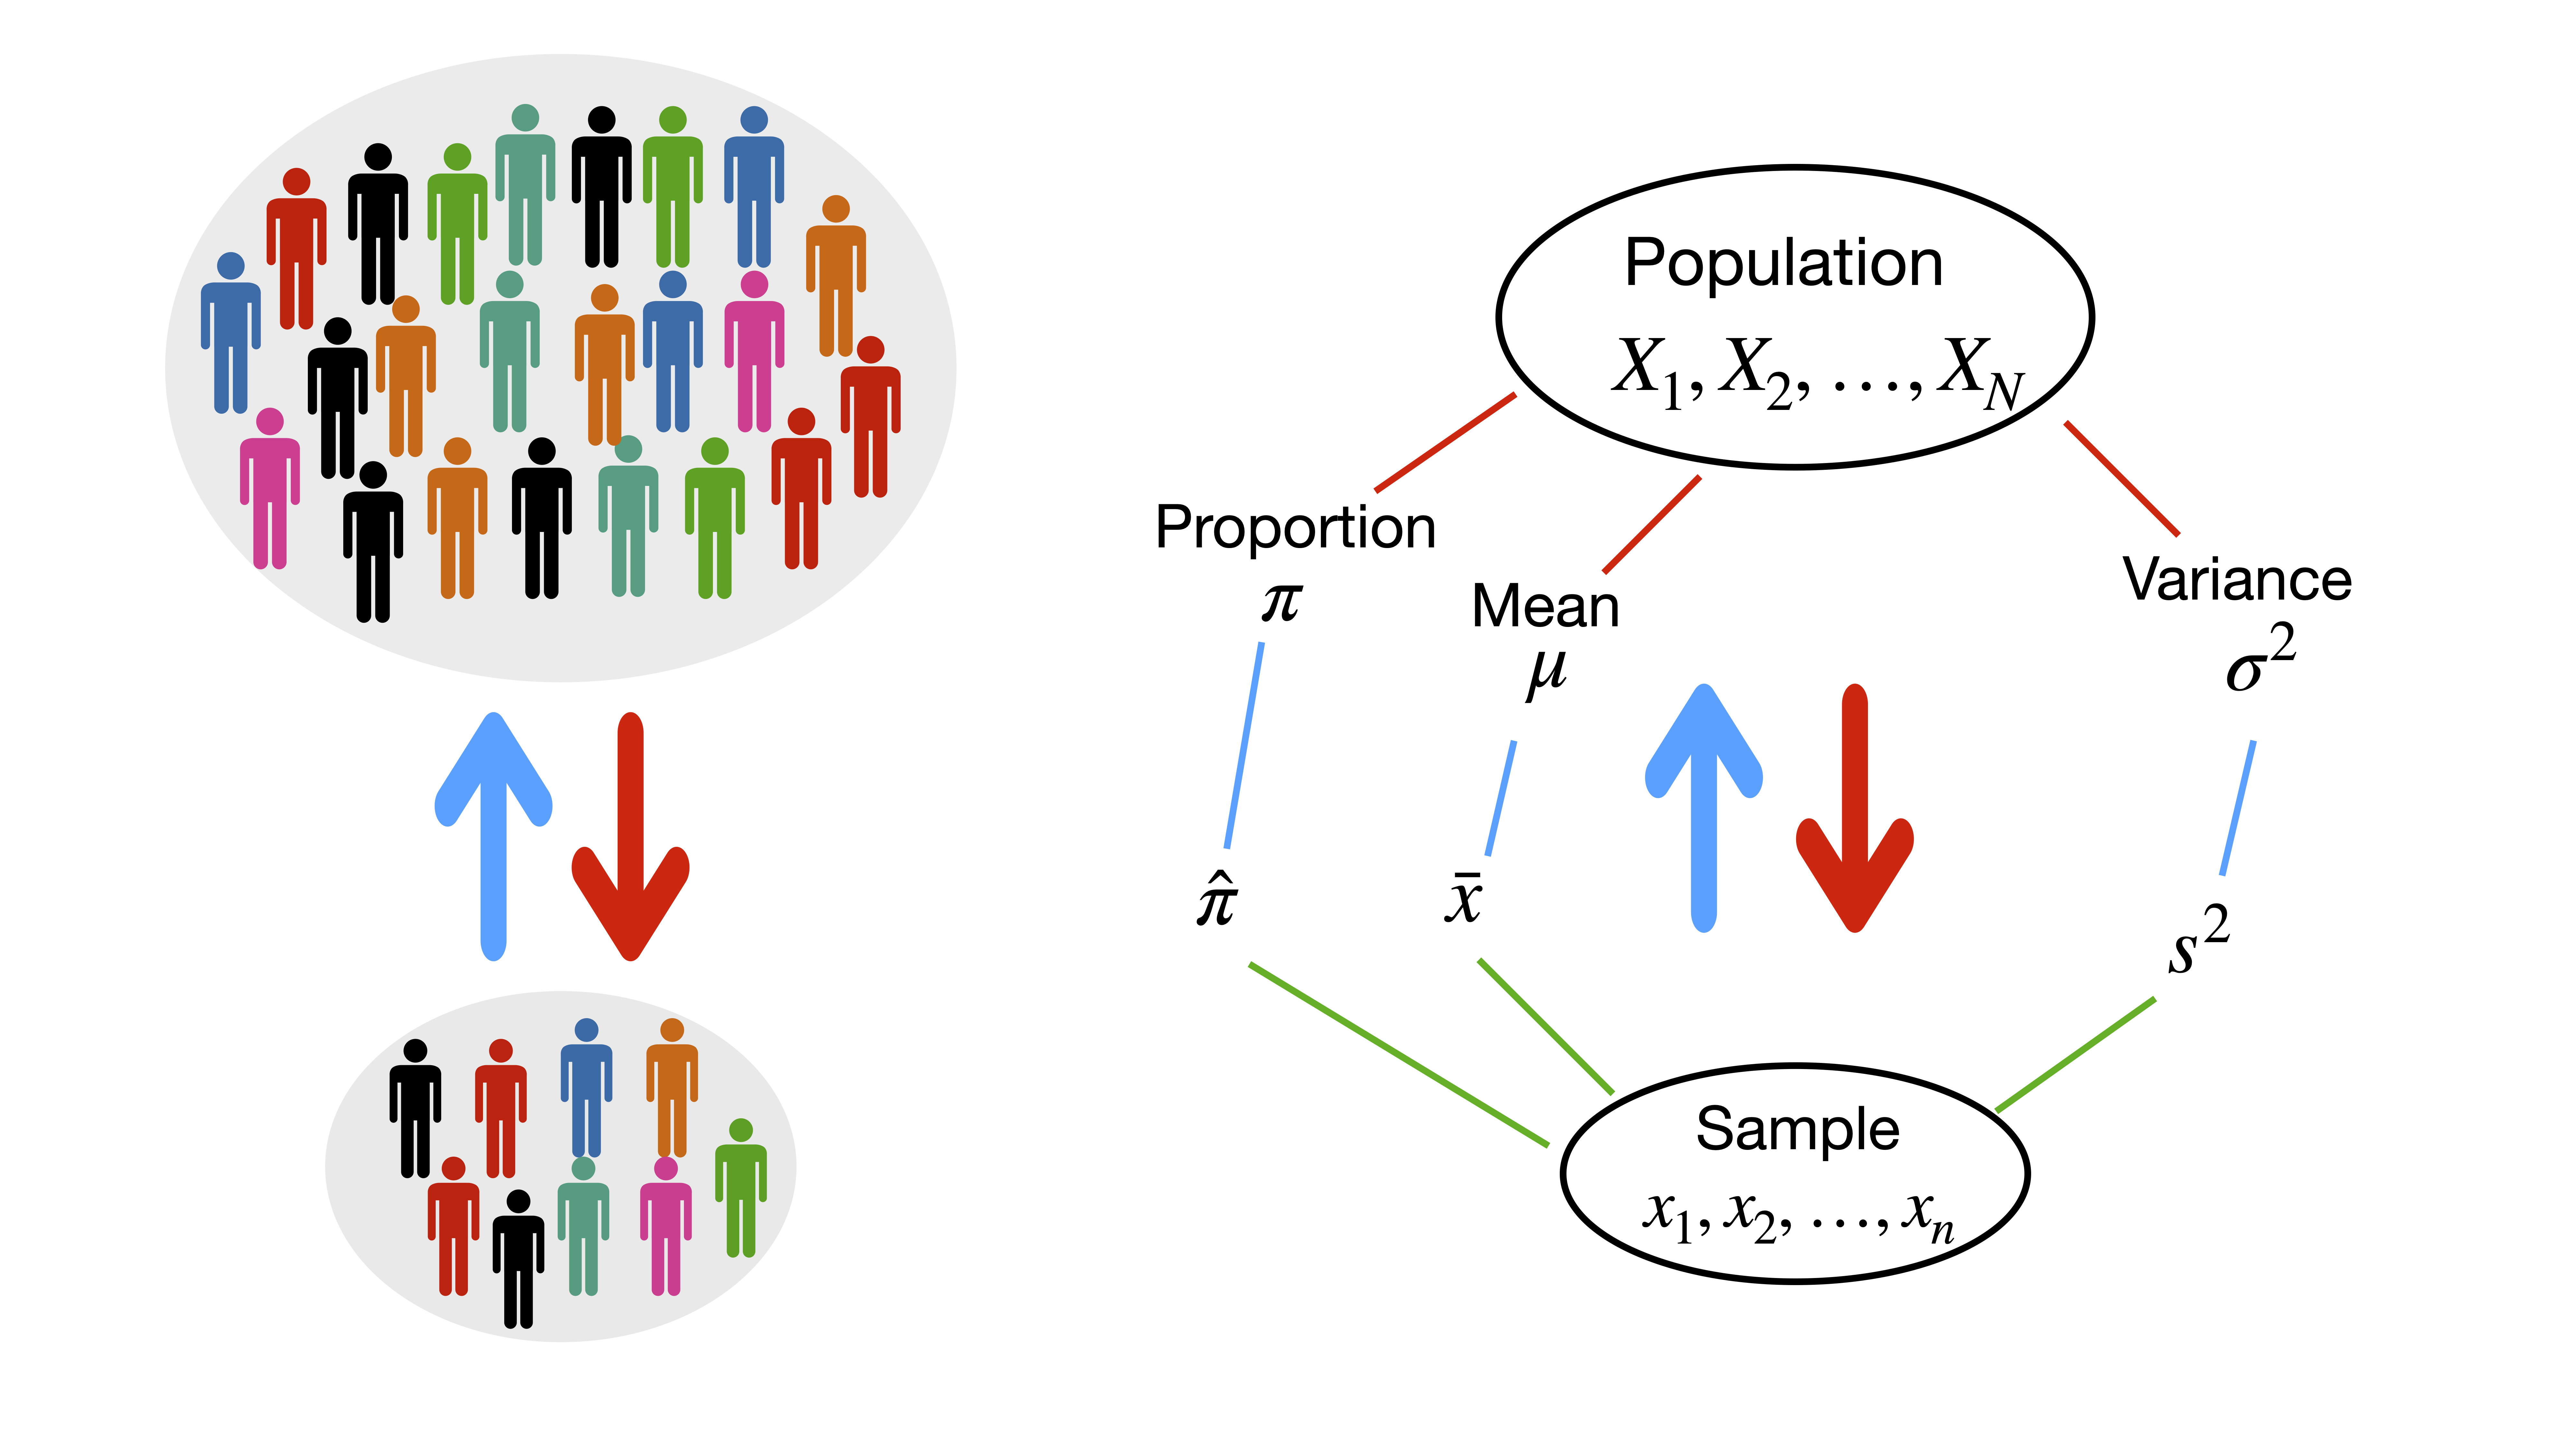
\includegraphics[width=0.65\linewidth,height=0.65\textheight]{stat1new} \end{center}

\hypertarget{notation}{%
\subsection{Notation}\label{notation}}

\begin{longtable}[]{@{}ccc@{}}
\toprule()
~ & Population & Sample \\
\midrule()
\endhead
Size & \(N\) & \(n\) \\
& Parameter & Statistic \\
Mean & \(\mu\) & \(\bar{x}\) \\
Variance & \(\sigma^2\) & \(s^2\) \\
Standard deviation & \(\sigma\) & \(s\) \\
Proportion & \(\pi\) & \(\hat{\pi}\) \\
Correlation & \(\rho\) & \(r\) \\
\bottomrule()
\end{longtable}

\pagebreak

\hypertarget{data-types-in-statistics}{%
\section{Data Types in Statistics}\label{data-types-in-statistics}}

\hypertarget{data-collection-methods-traditional-data}{%
\subsection{Data collection methods (Traditional
data)}\label{data-collection-methods-traditional-data}}

There are several ways for collecting data:

\begin{itemize}
\tightlist
\item
  \textbf{Take a census:} a census is a count or measure of an entire
  population. Taking a census provides complete information, but it is
  often costly and difficult to perform.
\item
  \textbf{Use sampling:} a sample is a count or measure of a part of a
  population. Statistics calculated from a sample are used to estimate
  population parameters.
\item
  \textbf{Use a simulation:} collecting data often involves the use of
  computers. Simulations allow studying situations that are impractical
  or even dangerous to create in real life and often save time and
  money.
\item
  \textbf{Perform an experiment:} e.g.~to test the effect of imposing a
  new marketing strategy, one could perform an experiment by using the
  new marketing strategy in a certain region.
\end{itemize}

\hypertarget{data-collection-methods-big-data}{%
\subsection{Data collection methods (Big
data)}\label{data-collection-methods-big-data}}

The characteristics of big data (the 4Vs?):

\begin{itemize}
\tightlist
\item
  Volume: how much data is there?
\item
  Variety: different types of data?
\item
  Velocity: at what speed?
\item
  Veracity: how accurate?
\end{itemize}

\hypertarget{types-of-data}{%
\subsection{Types of data}\label{types-of-data}}

Data sets can consist of two types of data:

\begin{itemize}
\item
  \textbf{Qualitative (categorical) data} consist of attributes, labels,
  or nonnumerical entries. e.g.~name of cities, gender etc.
\item
  \textbf{Quantitative data} consist of numerical measurements or
  counts. e.g.~heights, weights, age. Quantitative data can be
  distinguished as:

  \begin{itemize}
  \item
    \textbf{Discrete data} result when the number of possible values is
    either a finite number or a ``countable'' number. e.g.~the number of
    phone calls you received in any given day.
  \item
    \textbf{Continuous data} result from infinitely many possible values
    that correspond to some continuous scale that covers a range of
    values without gaps, interruptions, or jumps. e.g.~height, weight,
    sales and market shares.
  \end{itemize}
\end{itemize}

\hypertarget{types-of-data-econometrics}{%
\subsection{Types of data
(Econometrics)}\label{types-of-data-econometrics}}

\begin{itemize}
\item
  \textbf{Cross-sectional data:} Data on different entities
  (e.g.~workers, consumers, firms, governmental units) for a single time
  period. For example, data on test scores in different school
  districts.
\item
  \textbf{Time series data:} Data for a single entity (e.g.~person,
  firm, country) collected at multiple time periods. For example, the
  rate of inflation and unemployment for a country over the last 10
  years.
\item
  \textbf{Panel data:} Data for multiple entities in which each entity
  is observed at two or more time periods. For example, the daily prices
  of a number of stocks over two years.
\end{itemize}

\hypertarget{levels-of-measurement}{%
\subsection{Levels of measurement}\label{levels-of-measurement}}

\begin{itemize}
\item
  \textbf{Nominal:} Categories only, data cannot be arranged in an
  ordering scheme. (e.g.~Marital status: single, married etc.)
\item
  \textbf{Ordinal:} Categories are ordered, but differences cannot be
  determined or they are meaningless (e.g.~poor, average, good)
\item
  \textbf{Interval:} differences between values are meaningful, but
  there is no natural starting point, ratios are meaningless (e.g.~we
  cannot say that the temperature 80\(^{\circ}\)F is twice as hot as
  40\(^{\circ}\)F)
\item
  \textbf{Ratio:} Like interval level, but there is a natural zero
  starting point and rations are meaningful (e.g.~\textsterling20 is
  twice as much as \textsterling10)
\end{itemize}

\pagebreak

\hypertarget{descriptive-statistics}{%
\section{Descriptive Statistics}\label{descriptive-statistics}}

\hypertarget{measures-of-central-tendency}{%
\subsection{Measures of Central
Tendency}\label{measures-of-central-tendency}}

Measures of central tendency provide numerical information about a
`typical' observation in the data.

\begin{itemize}
\tightlist
\item
  The \textbf{Mean} (also called the average) of a data set is the sum
  of the data values divided by the number of observations.
\end{itemize}

\[\;\;\;\; \text{Sample mean:}\;\;\; \bar{x}=\frac{1}{n}\sum_{i=1}^{n}x_i\]

\begin{itemize}
\tightlist
\item
  The \textbf{Median} is the middle observation when the data set is
  sorted in ascending or descending order. If the data set has an even
  number of observations, the median is the mean of the two middle
  observations.
\item
  The \textbf{Mode} is the data value that occurs with the greatest
  frequency. If no entry is repeated, the data set has no mode. If two
  (more than two) values occur with the same greatest frequency, each
  value is a mode and the data set is called bimodal (multimodal).
\end{itemize}

\hypertarget{measure-of-variation-dispersion}{%
\subsection{Measure of Variation
(Dispersion)}\label{measure-of-variation-dispersion}}

The variation (dispersion) of a set of observations refers to the
variability that they exhibit.

\begin{itemize}
\item
  \textbf{Range} = maximum data value - minimum data value
\item
  The \textbf{variance} measures the variability or spread of the
  observations from the mean.
\end{itemize}

\[\text{Sample variance:}\;\;\;s^2=\frac{1}{n-1}\sum_{i=1}^{n}(x_i-\bar{x})^2\]

\begin{itemize}
\item
  Shortcut formula for sample variance is given by
  \[\text{Sample variance:}\;\;\;s^2=\frac{1}{n-1}\left\{\sum_{i=1}^{n}x^2_i-n\bar{x}^2\right\}\]
\item
  The \textbf{standard deviation} (\(s\)) of a data set is the square
  root of the sample variance.
\end{itemize}

\hypertarget{shape-of-a-distribution-skewness}{%
\subsection{Shape of a distribution:
Skewness}\label{shape-of-a-distribution-skewness}}

Skewness is a measure of the asymmetry of the distribution.

\begin{center}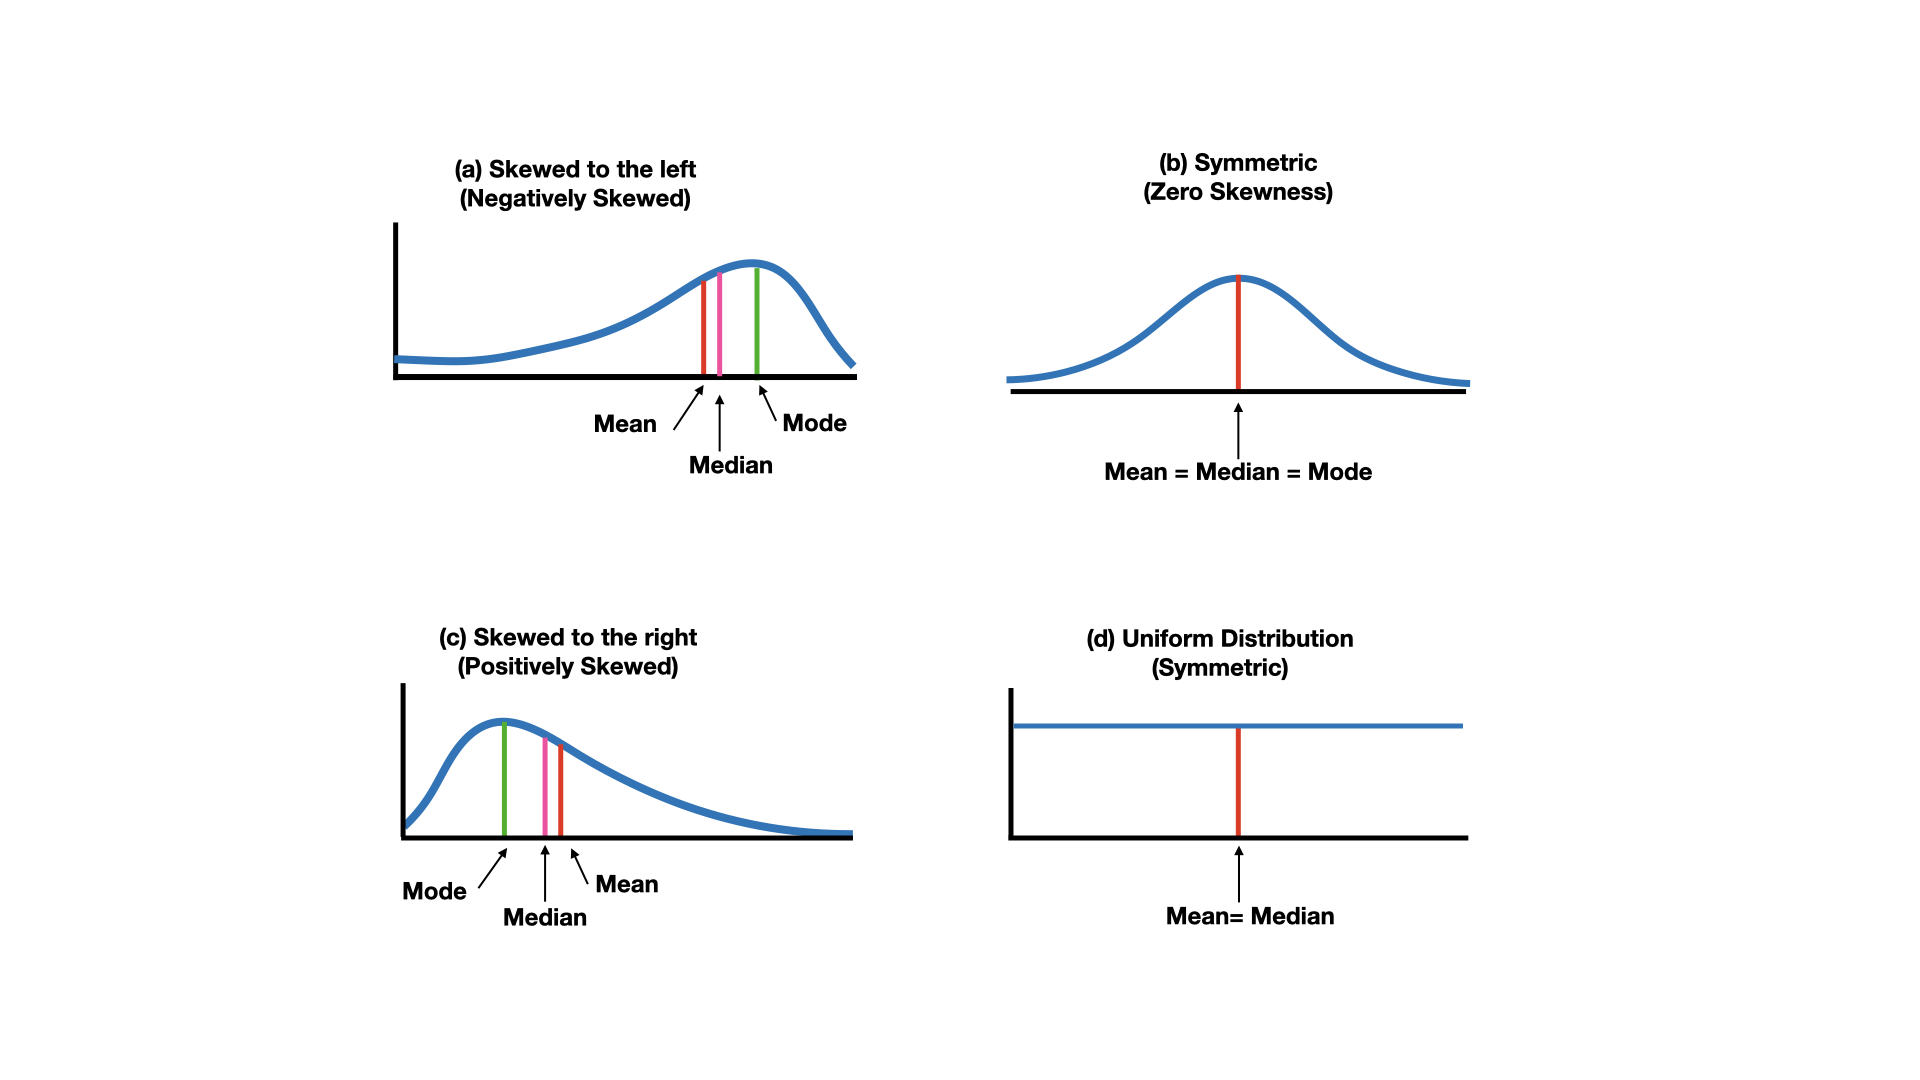
\includegraphics[width=1.3\linewidth,height=1.3\textheight]{skewed} \end{center}

\hypertarget{shape-of-a-distribution-kurtosis}{%
\subsection{Shape of a distribution:
Kurtosis}\label{shape-of-a-distribution-kurtosis}}

Kurtosis measures the degree of peakedness or flatness of the
distribution.

\begin{center}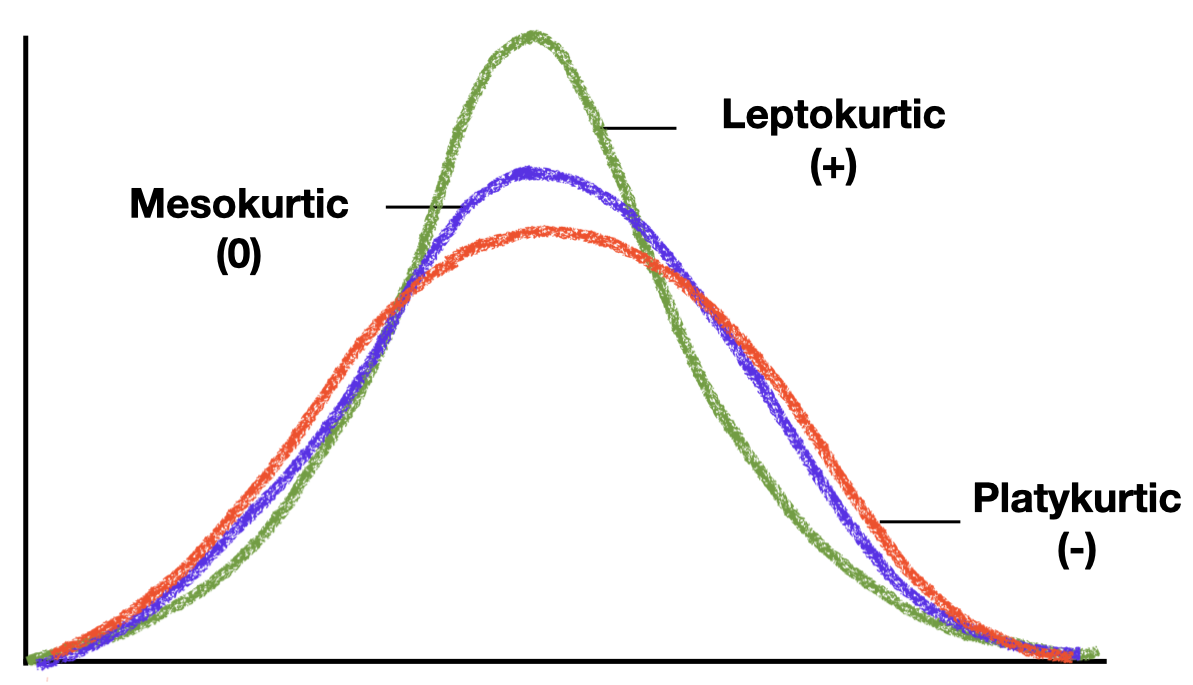
\includegraphics[width=1\linewidth,height=0.6\textheight]{kurtosis1} \end{center}

\hypertarget{modality}{%
\subsection{Modality}\label{modality}}

\begin{center}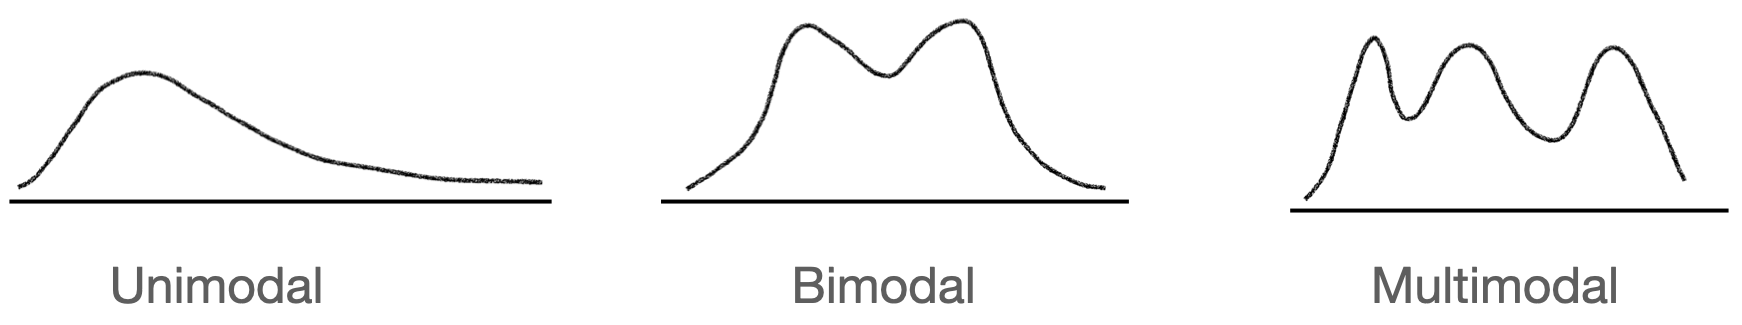
\includegraphics[width=1.3\linewidth,height=0.6\textheight]{modality} \end{center}

\hypertarget{symmetry}{%
\subsection{Symmetry}\label{symmetry}}

\begin{center}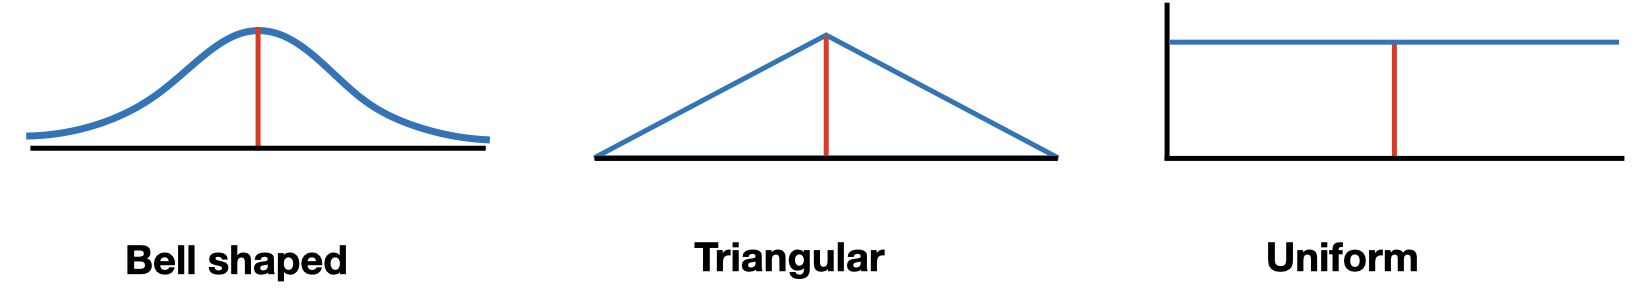
\includegraphics[width=1.3\linewidth,height=0.6\textheight]{symmetry} \end{center}

\hypertarget{empirical-rule}{%
\subsection{Empirical Rule}\label{empirical-rule}}

The empirical rule states (for a normally distributed data) that 68\% of
the data falls within one standard deviation; 95\% of the data falls
within two standard deviations; 99.7\% of the data falls within three
standard deviations from the mean.

\begin{center}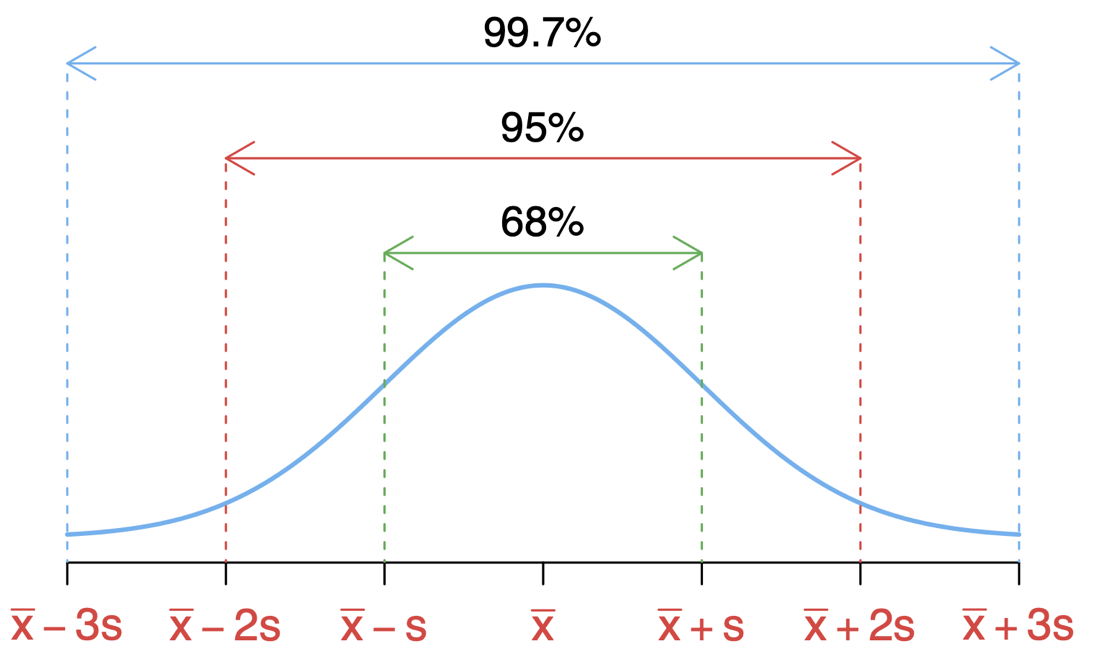
\includegraphics[width=0.6\linewidth,height=0.6\textheight]{bell} \end{center}

\hypertarget{measure-of-position-z-score}{%
\subsection{\texorpdfstring{Measure of Position:
\(z\)-score}{Measure of Position: z-score}}\label{measure-of-position-z-score}}

The \textbf{\(z\)-score} of an observation tells us the number of
standard deviations that the observation is from the mean, that is, how
far the observation is from the mean in units of standard deviation.

\[z=\frac{x-\bar{x}}{s}\]

As the \(z\)-score has no unit, it can be used to compare values from
different data sets or to compare values within the same data set. The
mean of \(z\)-scores is 0 and the standard deviation is 1.

Note that \(s>0\) so if \(z\) is negative, the corresponding \(x\)-value
is below the mean. If \(z\) is positive, the corresponding \(x\)-value
is above the mean. And if \(z=0\), the corresponding \(x\)-value is
equal to the mean.

\hypertarget{percentiles-and-quartiles}{%
\subsection{Percentiles and Quartiles}\label{percentiles-and-quartiles}}

\begin{itemize}
\tightlist
\item
  Given a set of observations, the \(k\)th percentile, \(P_k\) , is the
  value of \(X\) such that \(k\)\% or less of the observations are less
  than \(P_k\) and \((100-k)\)\% or less of the observations are greater
  than \(P_k\)
\end{itemize}

\begin{center}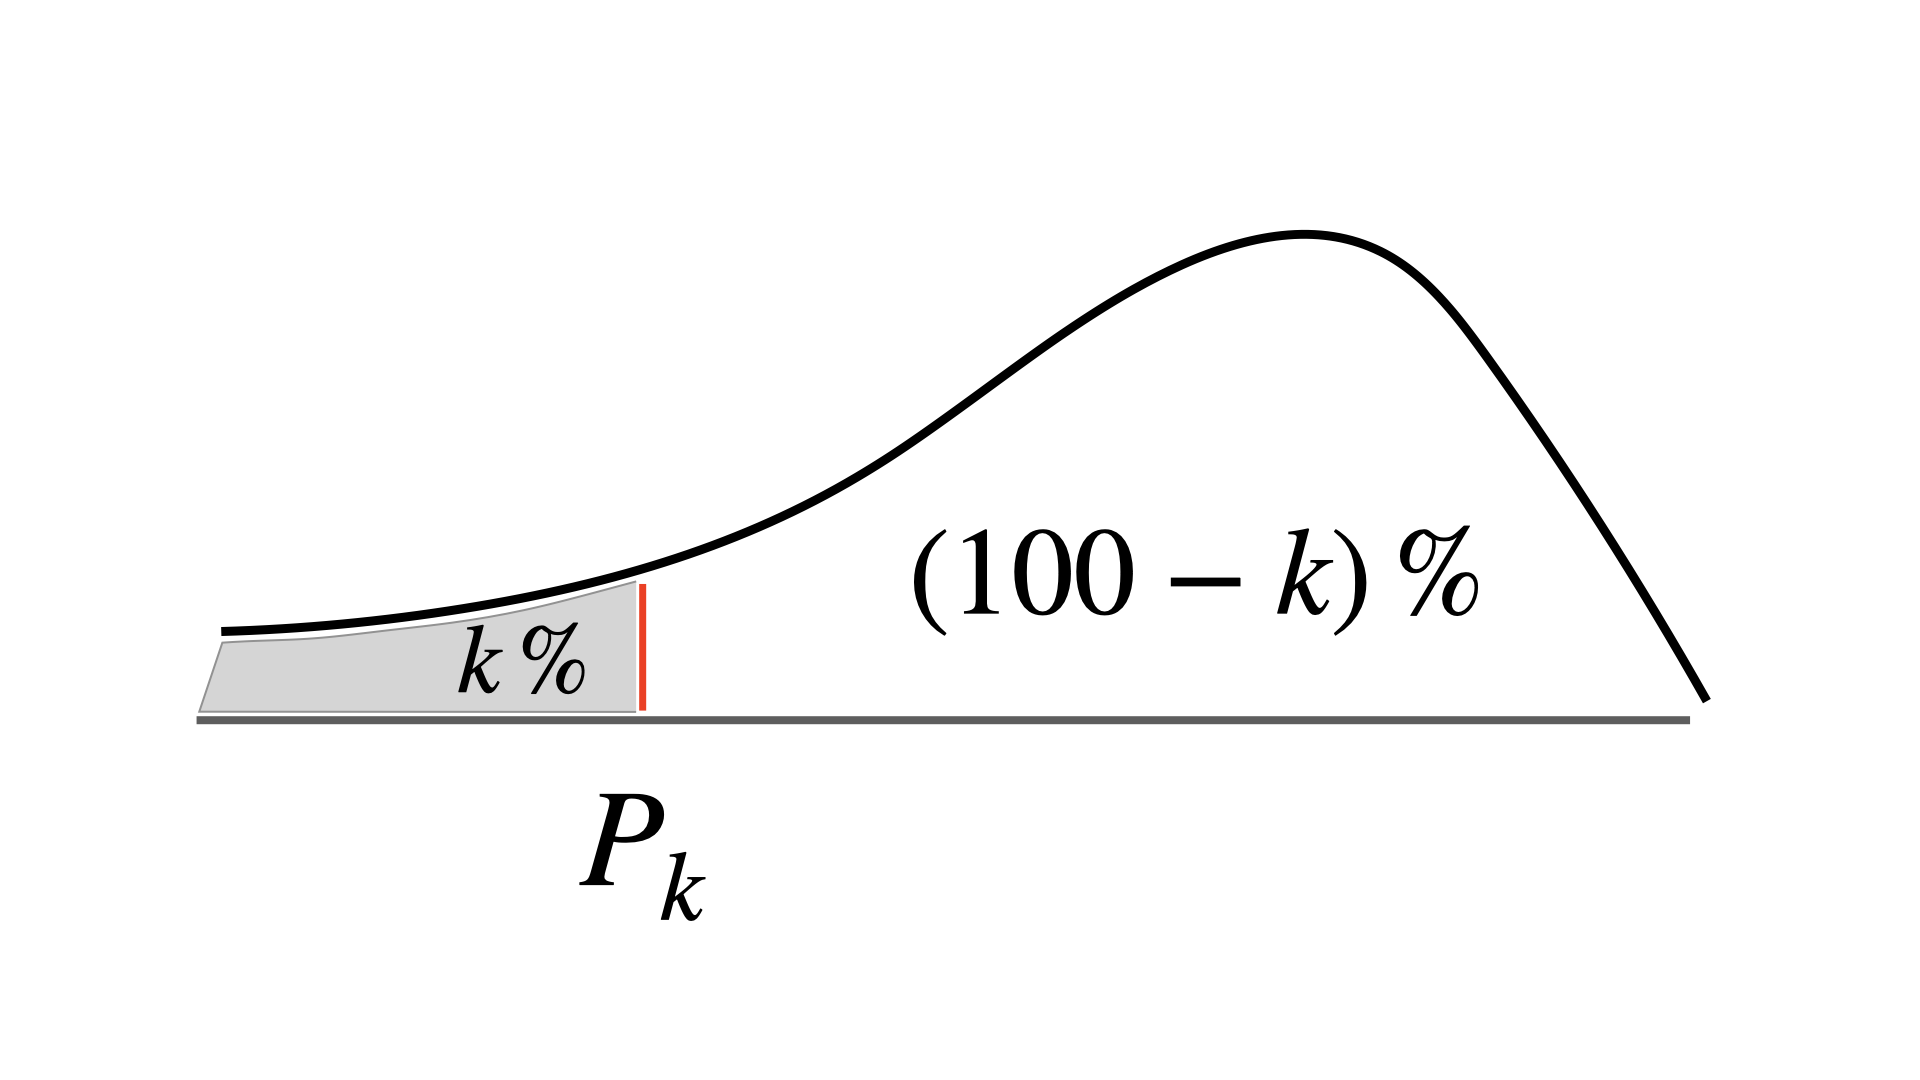
\includegraphics[width=1\linewidth,height=1\textheight]{qunatiles} \end{center}

\begin{itemize}
\item
  The 25th percentile, \(Q_1\), is often referred to as the first
  quartile.
\item
  The 50th percentile (the median), \(Q_2\), is referred to as the
  second or middle quartile.
\item
  The 75th percentile, \(Q_3\), is referred to as the third quartile
\end{itemize}

\hypertarget{a-toy-example}{%
\subsubsection{A toy example}\label{a-toy-example}}

\begin{center}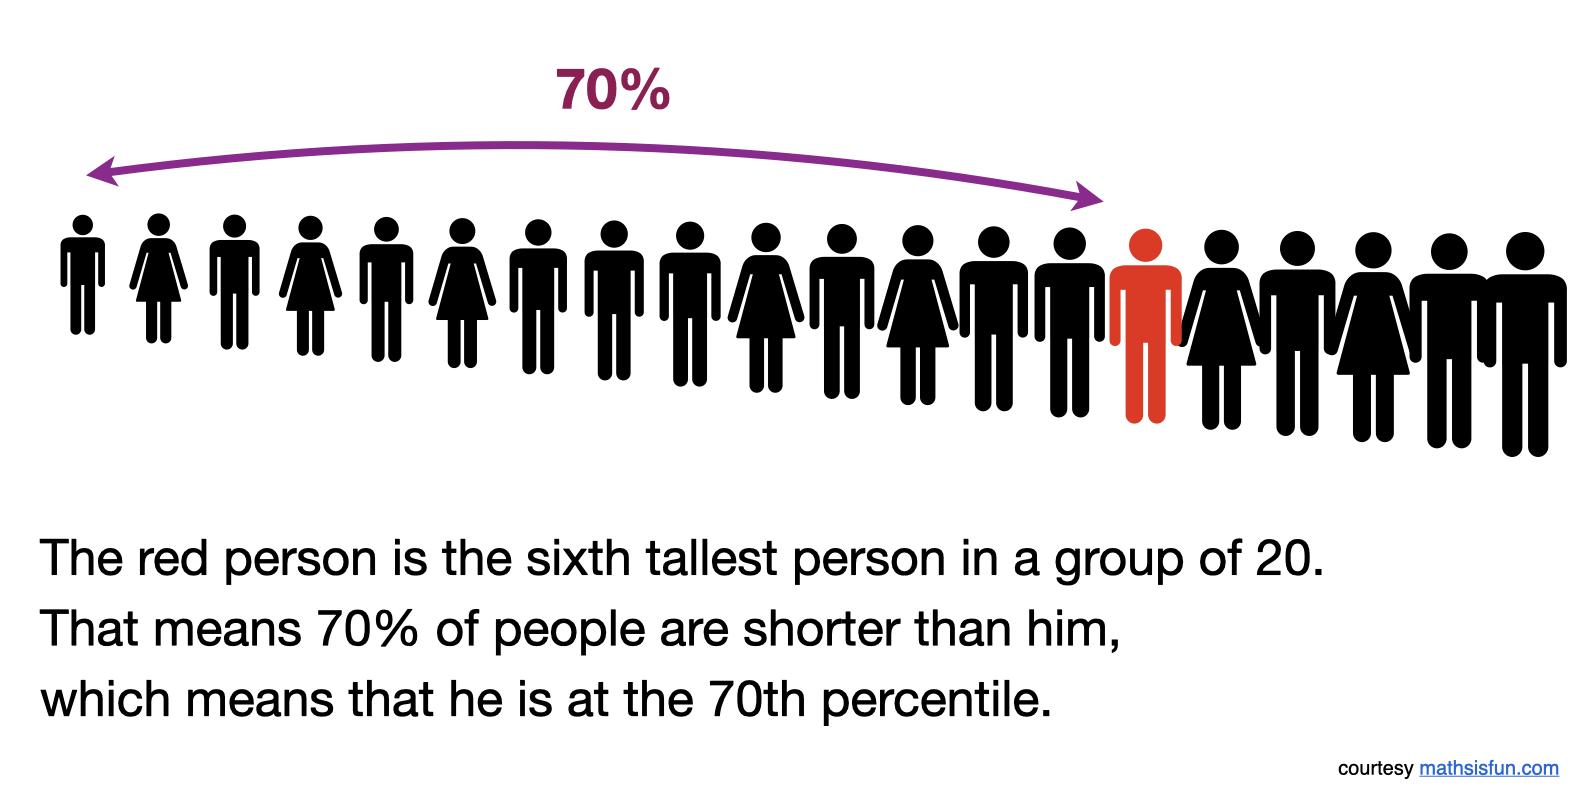
\includegraphics[width=0.6\linewidth,height=0.6\textheight]{toyexample} \end{center}

\hypertarget{the-quartiles-divide-a-data-set-into-quarters-four-equal-parts.}{%
\subsubsection{The quartiles divide a data set into quarters (four equal
parts).}\label{the-quartiles-divide-a-data-set-into-quarters-four-equal-parts.}}

\begin{center}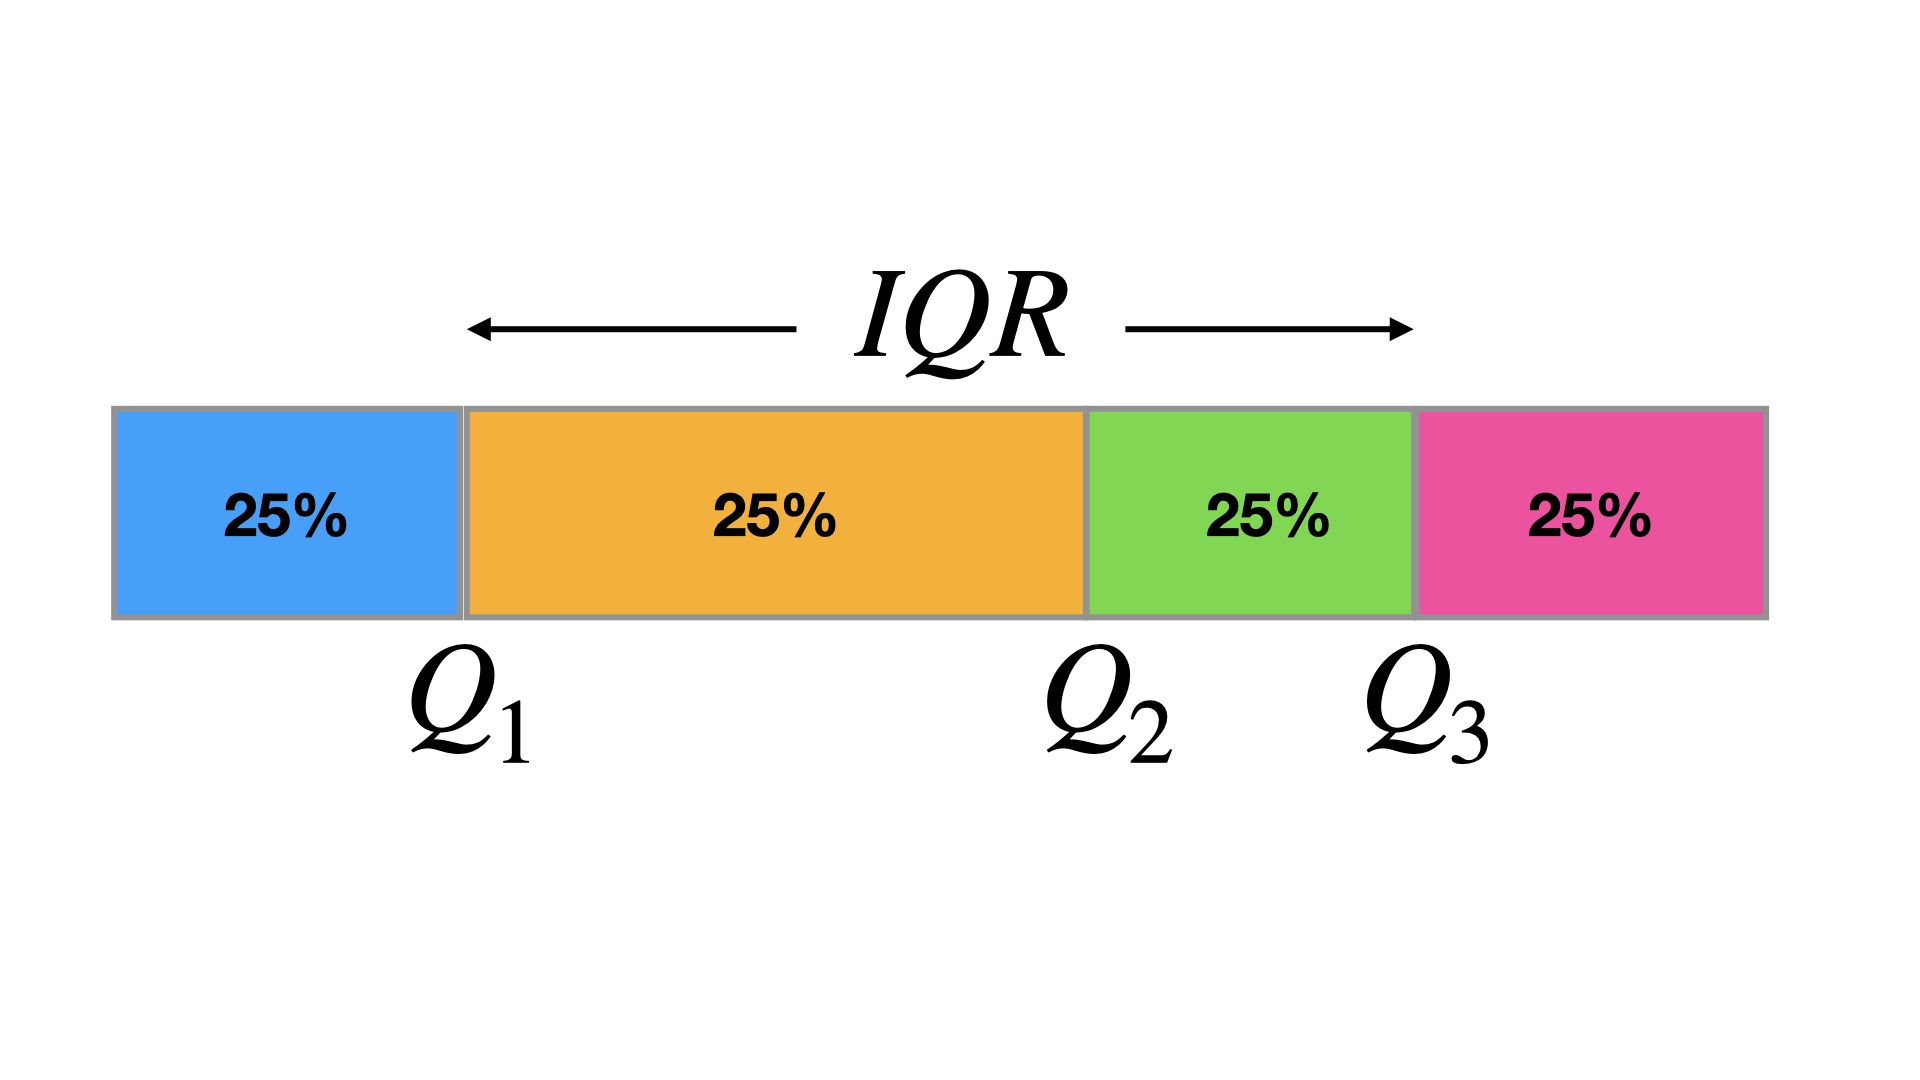
\includegraphics[width=0.6\linewidth,height=0.6\textheight]{QQ} \end{center}

\begin{itemize}
\item
  The interquartile range (\(IQR\)) of a data set is the difference
  between the first and third quartiles (\(IQR = Q_3 - Q_1\))
\item
  The IQR is a measure of variation that gives you an idea of how much
  the middle 50\% of the data varies.
\end{itemize}

\hypertarget{five-number-summary-boxplots}{%
\subsection{Five-number summary \&
Boxplots}\label{five-number-summary-boxplots}}

To graph a boxplot (a box-and-whisker plot), we need the following
values (called the five-number summary):

\begin{itemize}
\tightlist
\item
  The minimum entry
\item
  The first quartile \(Q_1\)
\item
  The median (second quartile ) \(Q_2\)
\item
  The maximum entry
\item
  The third quartile \(Q_3\)
\end{itemize}

\begin{center}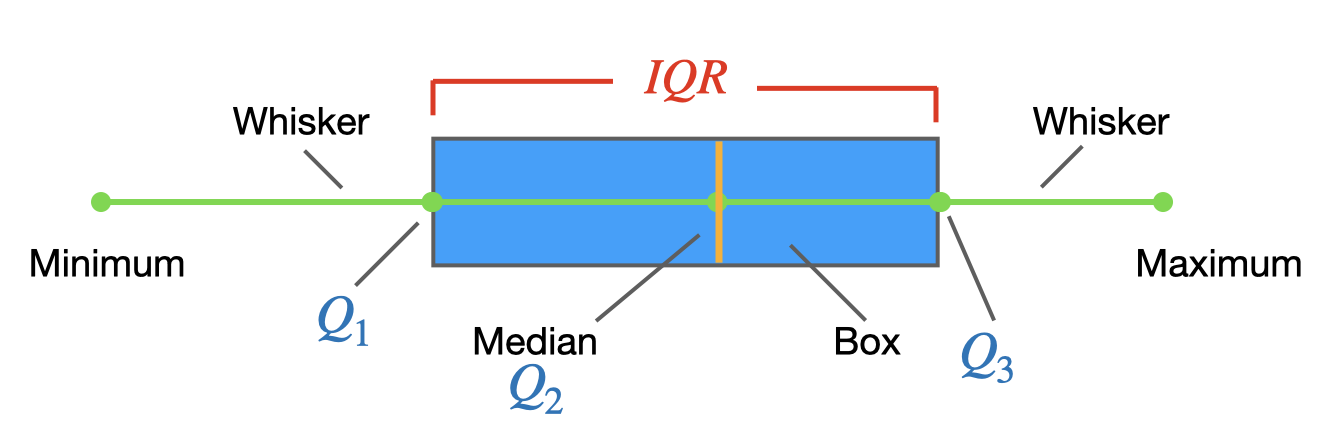
\includegraphics[width=0.6\linewidth,height=0.6\textheight]{boxplot3} \end{center}

The box represents the interquartile range (\(IQR\)), which contains the
middle 50\% of values.

\hypertarget{outliers-extremes-values}{%
\subsection{Outliers \& Extremes
values}\label{outliers-extremes-values}}

Some data sets contain outliers or extremes values, observations that
fall well outside the overall pattern of the data. Boxplots can help us
to identify such values if some rules-of-thumb are used, e.g.:

\begin{itemize}
\item
  Outlier: Cases with values between 1.5 and 3 box lengths (the box
  length is the interquartile range) from the upper or lower edge of the
  box.
\item
  Extremes: Cases with values more than 3 box lengths from the upper or
  lower edge of the box.
\end{itemize}

\begin{center}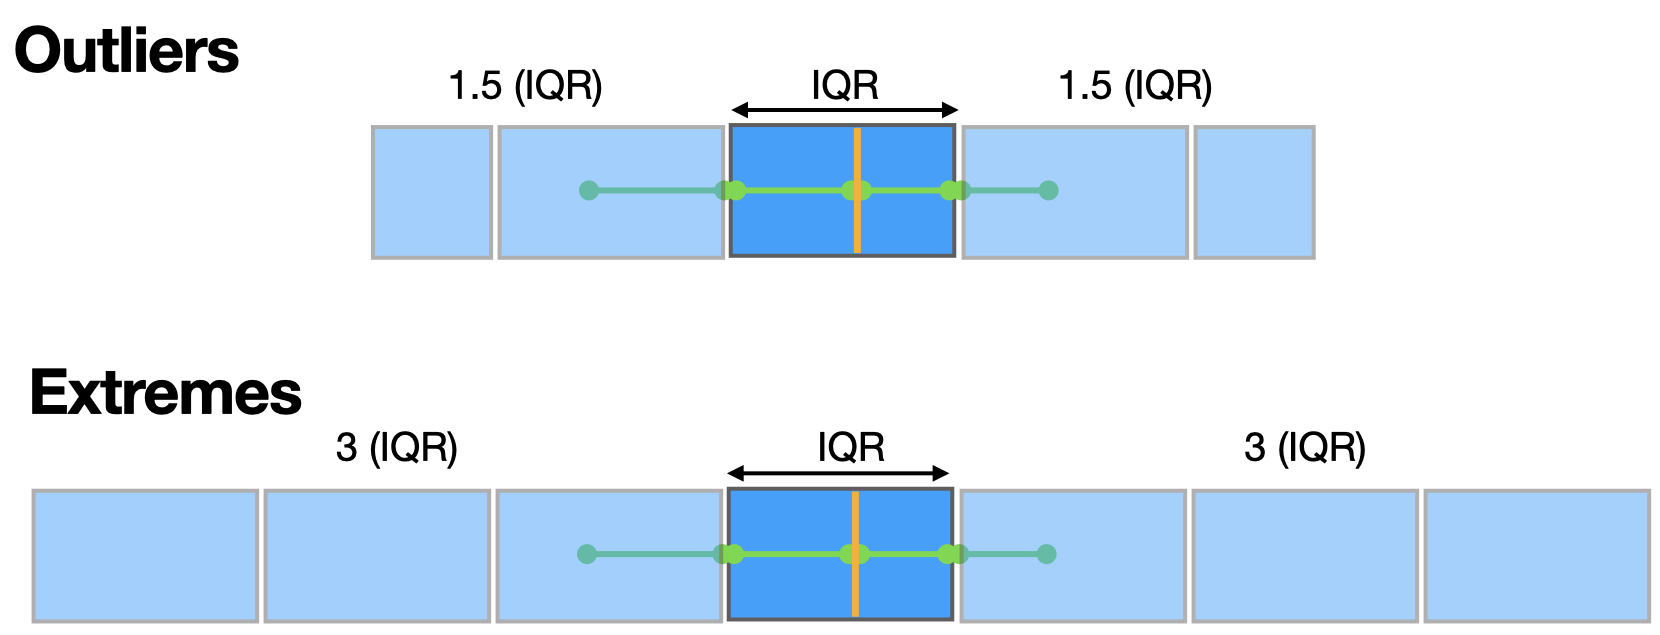
\includegraphics[width=0.6\linewidth,height=0.6\textheight]{outliers} \end{center}

\hypertarget{descriptive-statistics-for-qualitative-variables}{%
\subsection{Descriptive statistics for qualitative
variables}\label{descriptive-statistics-for-qualitative-variables}}

\begin{itemize}
\item
  Frequency distributions are tabular or graphical presentations of data
  that show each category for a variable and the frequency of the
  category's occurrence in the data set. Percentages for each category
  are often reported instead of, or in addition to, the frequencies.
\item
  The Mode can be used in this case as a measure of central tendency.
\item
  Bar charts and Pie charts are often used to display the results of
  categorical or qualitative variables. Pie charts are more useful for
  displaying results of variables that have relatively few categories,
  in that pie charts become cluttered and difficult to read if variables
  have many categories.
\end{itemize}

\hypertarget{example-accounting-final-exam-grades}{%
\subsection{Example: Accounting final exam
grades}\label{example-accounting-final-exam-grades}}

The accounting final exam grades of 10 students are: 88, 51, 63, 85, 79,
65, 79, 70, 73, and 77. Their study programs, respectively, are: MA, MA,
MBA, MBA, MBA, MBA, MBA, MSc, MSc, and MSc.

\begin{itemize}
\item
  The sample mean grade is
  \[\bar{x}=\frac{1}{n}\sum_{i=1}^{n}x_i=\frac{1}{10}(88+51+\ldots+77)=73\]
\item
  Next we arrange the data from the lowest to the largest grade: 51, 63,
  65, 70, \textbf{73}, \textbf{77}, 79, 79, 85, 88. The median grade is
  75, which located midway between the 5th and 6th ordered data points
  \((73+77)/2=75\).
\item
  The mode is 79 since it appears twice and all other grades appeared
  only once.
\item
  The range is \(88-51=37\).
\item
  The variance
  \[s^2=\frac{1}{n-1}\sum_{i=1}^{n}(x_i-\bar{x})^2=\frac{1}{9}((88-73)^2+\ldots+(77-73)^2)=123.78\]
\item
  The standard deviation: \(s=\sqrt{123.78}=11.13\)
\item
  The coefficient of variation: \(CV=s/\bar{x}=11.13/73=0.1525\)
\item
  Empirical rule: the empirical rule states (for a normally distributed
  data) that 68\% of the data falls within one standard deviation from
  the mean. In our example, this means that 68\% of the grades fall
  between 61.87 and 84.13 (\(73\pm 11.12555\))
\end{itemize}

\begin{center}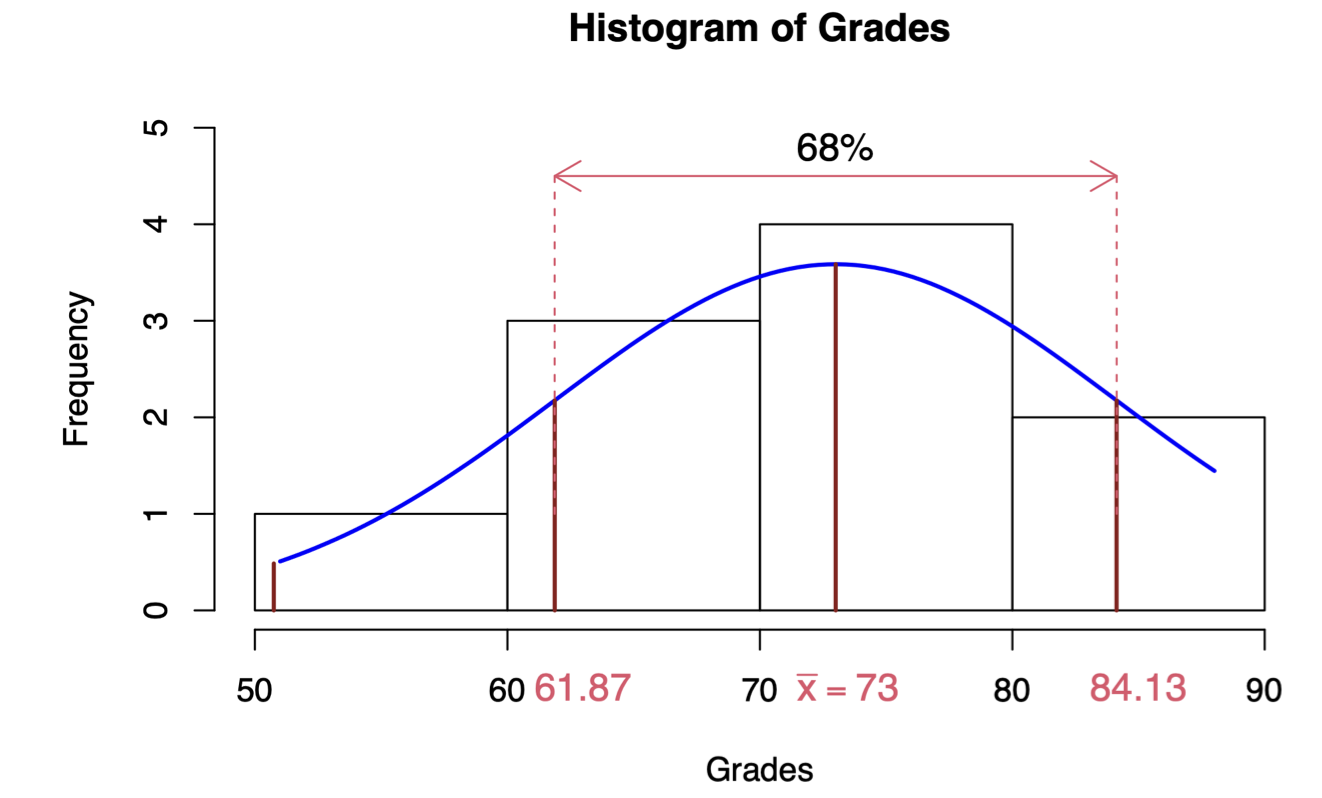
\includegraphics[width=1\linewidth,height=1\textheight]{Exempirical} \end{center}
 
%\begin{snugshade}
\begin{Highlighting}[]
\CommentTok{\# R codes for "Accounting final exam grades" example}
\CommentTok{\# Data example}
\NormalTok{grades}\OtherTok{\textless{}{-}}\FunctionTok{c}\NormalTok{(}\DecValTok{88}\NormalTok{,}\DecValTok{51}\NormalTok{,}\DecValTok{63}\NormalTok{,}\DecValTok{85}\NormalTok{,}\DecValTok{79}\NormalTok{,}\DecValTok{65}\NormalTok{,}\DecValTok{79}\NormalTok{,}\DecValTok{70}\NormalTok{,}\DecValTok{73}\NormalTok{,}\DecValTok{77}\NormalTok{)}
\NormalTok{program}\OtherTok{\textless{}{-}}\FunctionTok{factor}\NormalTok{(}\FunctionTok{c}\NormalTok{(}\StringTok{"MA"}\NormalTok{,}\StringTok{"MA"}\NormalTok{,}\StringTok{"MBA"}\NormalTok{,}\StringTok{"MBA"}\NormalTok{,}\StringTok{"MBA"}\NormalTok{,}\StringTok{"MBA"}\NormalTok{,}\StringTok{"MBA"}\NormalTok{,}\StringTok{"MSc"}\NormalTok{,}\StringTok{"MSc"}\NormalTok{,}\StringTok{"MSc"}\NormalTok{))}

\CommentTok{\# no of observations    }
\FunctionTok{length}\NormalTok{(grades)}
\end{Highlighting}
%\end{snugshade}

\begin{verbatim}
## [1] 10
\end{verbatim}

%\begin{Shaded}
\begin{Highlighting}[]
\CommentTok{\# Mean, Median, Variance, standard deviation, range, quantile}
\FunctionTok{mean}\NormalTok{(grades)}
\end{Highlighting}
%\end{Shaded}

\begin{verbatim}
## [1] 73
\end{verbatim}

%\begin{Shaded}
\begin{Highlighting}[]
\FunctionTok{median}\NormalTok{(grades)}
\end{Highlighting}
%\end{Shaded}

\begin{verbatim}
## [1] 75
\end{verbatim}

%\begin{Shaded}
\begin{Highlighting}[]
\FunctionTok{var}\NormalTok{(grades)}
\end{Highlighting}
%\end{Shaded}

\begin{verbatim}
## [1] 123.7778
\end{verbatim}

%\begin{Shaded}
\begin{Highlighting}[]
\FunctionTok{sd}\NormalTok{(grades)}
\end{Highlighting}
%\end{Shaded}

\begin{verbatim}
## [1] 11.12555
\end{verbatim}

%\begin{Shaded}
\begin{Highlighting}[]
\FunctionTok{range}\NormalTok{(grades)}
\end{Highlighting}
%\end{Shaded}

\begin{verbatim}
## [1] 51 88
\end{verbatim}

%\begin{Shaded}
\begin{Highlighting}[]
\FunctionTok{quantile}\NormalTok{(grades,}\AttributeTok{probs=}\FunctionTok{c}\NormalTok{(}\DecValTok{0}\NormalTok{,}\FloatTok{0.25}\NormalTok{,}\FloatTok{0.5}\NormalTok{,}\FloatTok{0.75}\NormalTok{,}\DecValTok{1}\NormalTok{))}
\end{Highlighting}
%\end{Shaded}

\begin{verbatim}
##    0%   25%   50%   75%  100% 
## 51.00 66.25 75.00 79.00 88.00
\end{verbatim}

%\begin{Shaded}
\begin{Highlighting}[]
\CommentTok{\# Summary}
\FunctionTok{summary}\NormalTok{(grades)}
\end{Highlighting}
%\end{Shaded}

\begin{verbatim}
##    Min. 1st Qu.  Median    Mean 3rd Qu.    Max. 
##   51.00   66.25   75.00   73.00   79.00   88.00
\end{verbatim}

%\begin{Shaded}
\begin{Highlighting}[]
\CommentTok{\# Calculate z{-}score}
\NormalTok{(grades}\SpecialCharTok{{-}}\FunctionTok{mean}\NormalTok{(grades))}\SpecialCharTok{/}\FunctionTok{sd}\NormalTok{(grades)}
\end{Highlighting}
%\end{Shaded}

\begin{verbatim}
##  [1]  1.3482484 -1.9774310 -0.8988323  1.0785987  0.5392994 -0.7190658
##  [7]  0.5392994 -0.2696497  0.0000000  0.3595329
\end{verbatim}

%\begin{Shaded}
\begin{Highlighting}[]
\FunctionTok{scale}\NormalTok{(grades)}
\end{Highlighting}
%\end{Shaded}

\begin{verbatim}
##             [,1]
##  [1,]  1.3482484
##  [2,] -1.9774310
##  [3,] -0.8988323
##  [4,]  1.0785987
##  [5,]  0.5392994
##  [6,] -0.7190658
##  [7,]  0.5392994
##  [8,] -0.2696497
##  [9,]  0.0000000
## [10,]  0.3595329
## attr(,"scaled:center")
## [1] 73
## attr(,"scaled:scale")
## [1] 11.12555
\end{verbatim}

 

%\begin{Shaded}
\begin{Highlighting}[]
\CommentTok{\#  Histograms present frequencies for values grouped into interval.}
\FunctionTok{hist}\NormalTok{(grades,}\AttributeTok{xlab=}\StringTok{"grades"}\NormalTok{, }\AttributeTok{main=}\StringTok{"Histogram of grades"}\NormalTok{)}
\end{Highlighting}
%\end{Shaded}

\begin{center}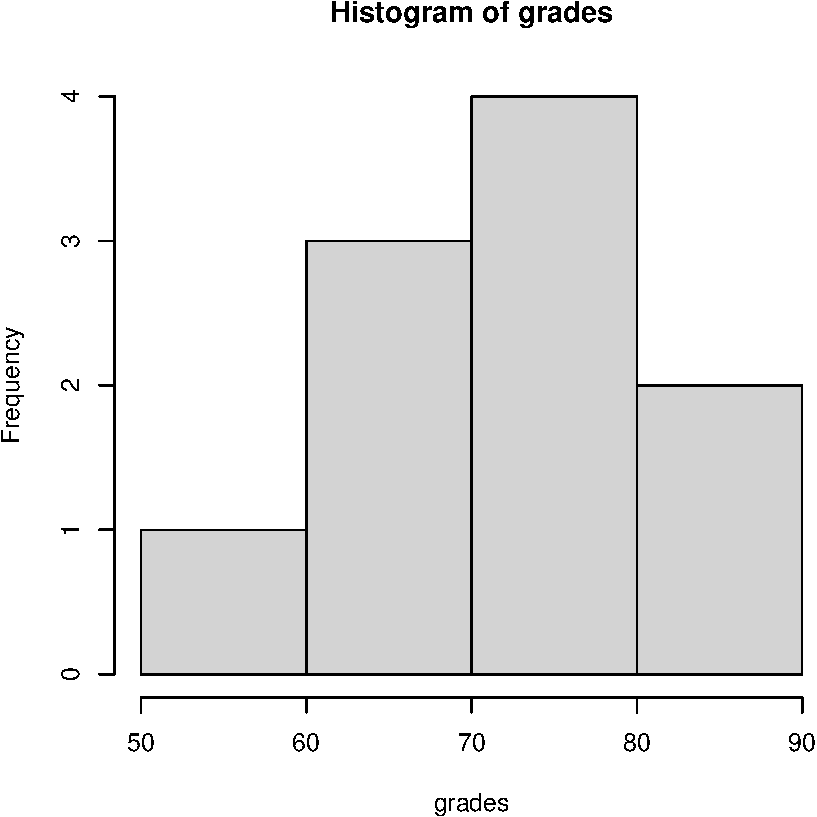
\includegraphics[width=1\linewidth,height=1\textheight]{unnamed-chunk-24-1} \end{center}

%\begin{Shaded}
\begin{Highlighting}[]
\CommentTok{\# Boxplot}
\FunctionTok{boxplot}\NormalTok{(grades,}\AttributeTok{xlab=}\StringTok{"grades"}\NormalTok{)}
\end{Highlighting}
%\end{Shaded}

\begin{center}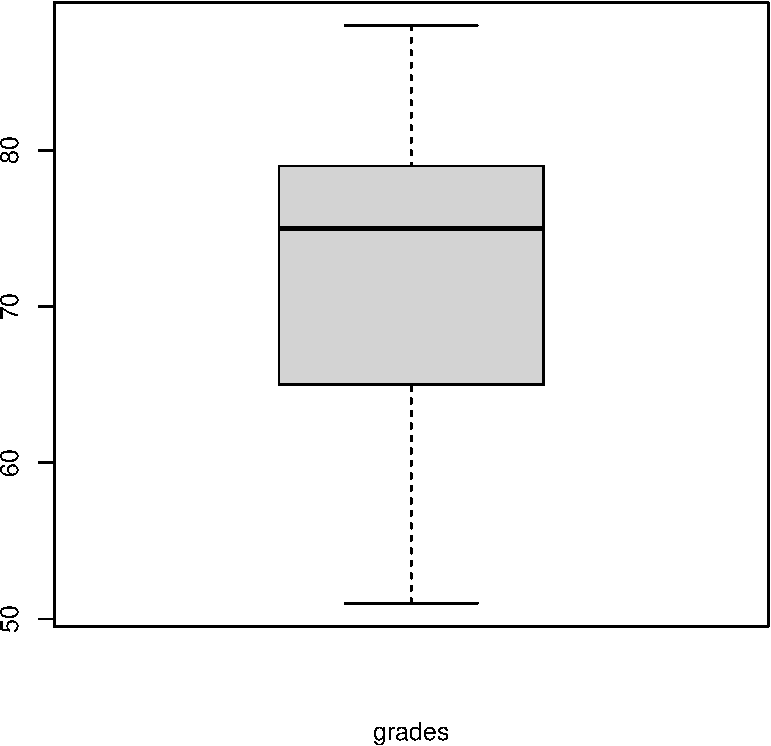
\includegraphics[width=1\linewidth,height=1\textheight]{unnamed-chunk-24-2} \end{center}



Stem-and-leaf plots: each score on a variable is divided into two parts,
the stem gives the leading digits and the leaf shows the trailing
digits.

The accounting final exam grades (arranged from the lowest to the
largest grade) are: 51, 63, 65, 70, 73, 77, 79, 79, 85, 88.

 

%\begin{Shaded}
\begin{Highlighting}[]
\CommentTok{\# Stem{-}and{-}leaf plot.}
\FunctionTok{stem}\NormalTok{(grades)}
\end{Highlighting}
%\end{Shaded}

\begin{verbatim}
## 
##   The decimal point is 1 digit(s) to the right of the |
## 
##   5 | 1
##   6 | 35
##   7 | 03799
##   8 | 58
\end{verbatim}

Dot plot: is a simple graph to show the relative positions of the data
points.

%\begin{Shaded}
\begin{Highlighting}[]
\NormalTok{col2}\OtherTok{\textless{}{-}}\FunctionTok{as.character}\NormalTok{(}\FunctionTok{factor}\NormalTok{(program,}\AttributeTok{labels=}\FunctionTok{c}\NormalTok{(}\StringTok{"red"}\NormalTok{,}\StringTok{"blue"}\NormalTok{,}\StringTok{"orange"}\NormalTok{)))}
\FunctionTok{dotchart}\NormalTok{(grades, }\AttributeTok{labels=}\FunctionTok{factor}\NormalTok{(}\DecValTok{1}\SpecialCharTok{:}\DecValTok{10}\NormalTok{), }\AttributeTok{groups=}\NormalTok{program, }\AttributeTok{pch=}\DecValTok{16}\NormalTok{, }\AttributeTok{col=}\NormalTok{col2, }\AttributeTok{xlab=}\StringTok{"Grades"}\NormalTok{,}\AttributeTok{xlim=}\FunctionTok{c}\NormalTok{(}\DecValTok{45}\NormalTok{,}\DecValTok{100}\NormalTok{))}
\end{Highlighting}
%\end{Shaded}

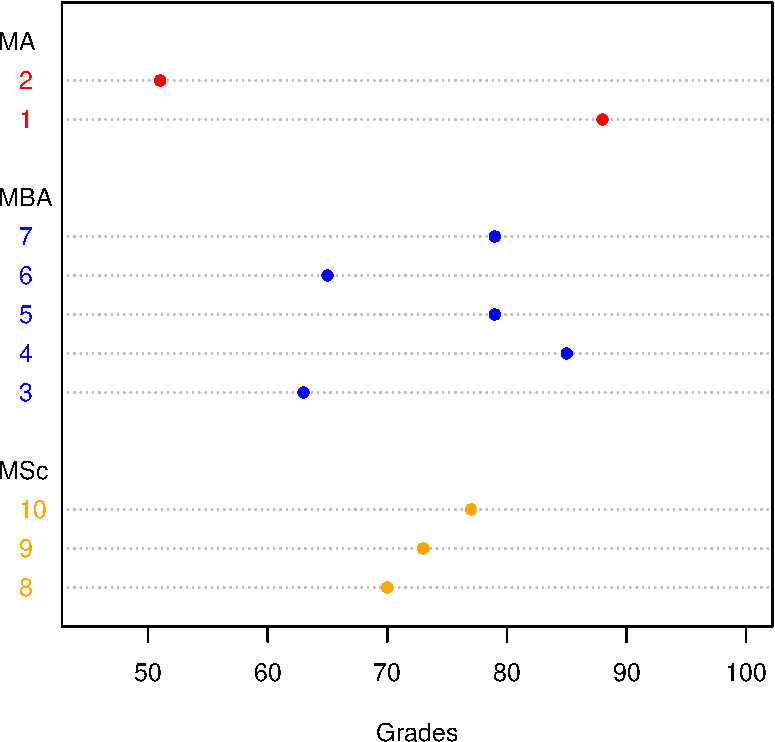
\includegraphics[width=1\linewidth,height=1\textheight]{unnamed-chunk-26-1}

 

%\begin{Shaded}
\begin{Highlighting}[]
\CommentTok{\# Frequency table}
\FunctionTok{table}\NormalTok{(program)}
\end{Highlighting}
%\end{Shaded}

\begin{verbatim}
## program
##  MA MBA MSc 
##   2   5   3
\end{verbatim}

%\begin{Shaded}
\begin{Highlighting}[]
\CommentTok{\# Pie and Bar charts}
\FunctionTok{pie}\NormalTok{(}\FunctionTok{table}\NormalTok{(program))}
\end{Highlighting}
%\end{Shaded}

\begin{center}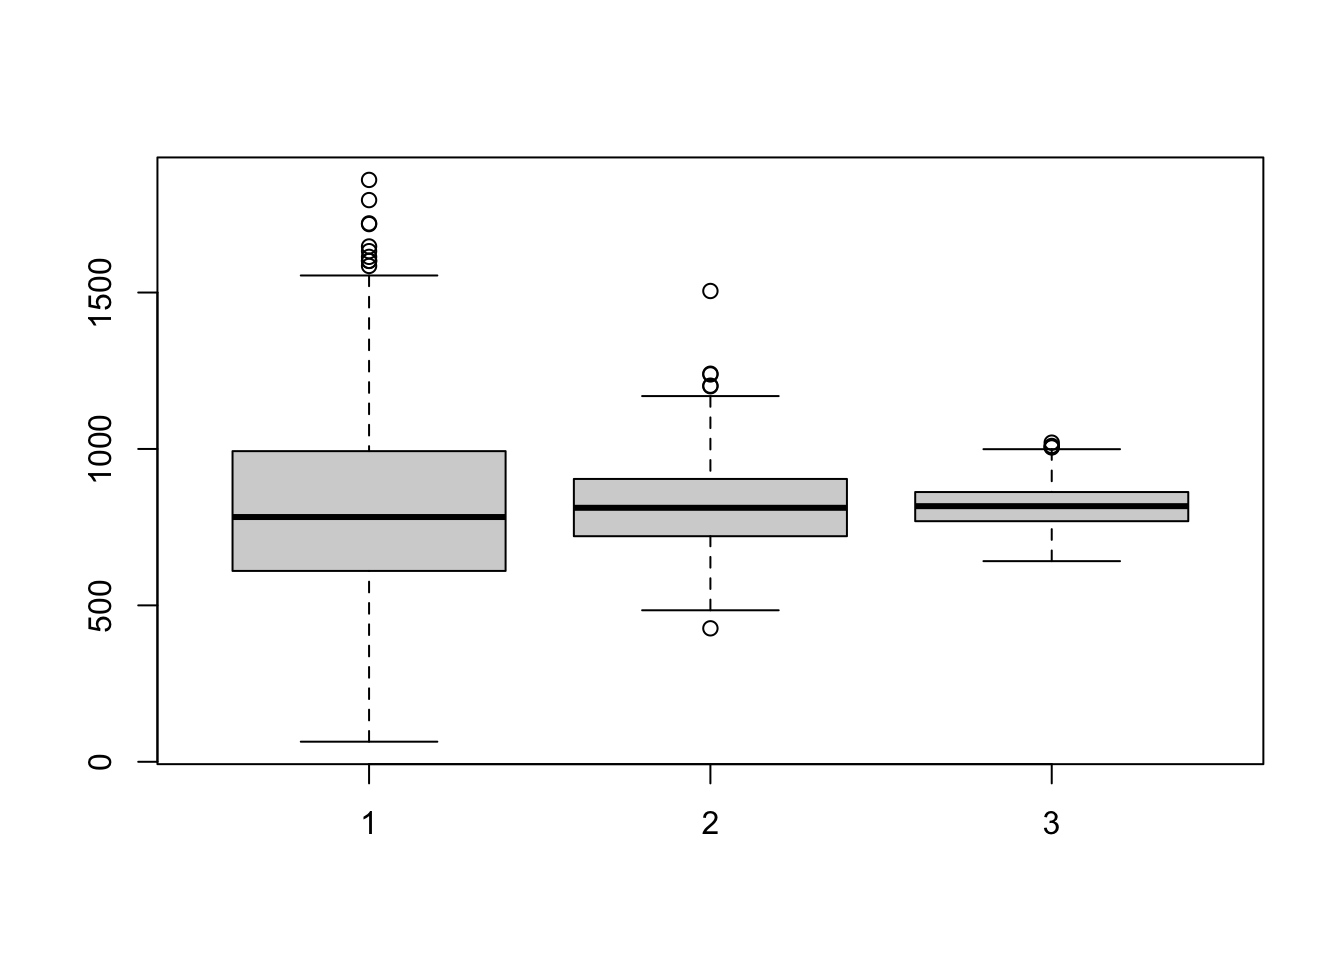
\includegraphics[width=0.5\linewidth,height=0.5\textheight]{unnamed-chunk-27-1} \end{center}

%\begin{Shaded}
\begin{Highlighting}[]
\FunctionTok{barplot}\NormalTok{(}\FunctionTok{table}\NormalTok{(program))}
\end{Highlighting}
%\end{Shaded}

\begin{center}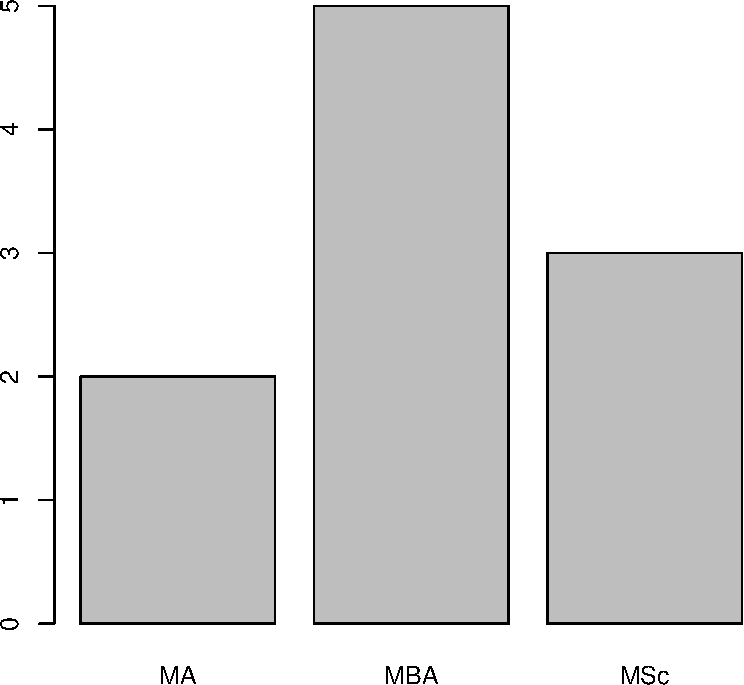
\includegraphics[width=1\linewidth,height=1\textheight]{unnamed-chunk-27-2} \end{center}

\pagebreak

\hypertarget{continuous-distributions}{%
\section{Continuous Distributions}\label{continuous-distributions}}

\hypertarget{random-variables}{%
\subsection{Random Variables}\label{random-variables}}

\begin{itemize}
\tightlist
\item
  A \textbf{random variable} is a variable whose possible values are
  numerical outcomes of a random experiment.
\item
  The term `random' is used here to imply the uncertainty associated
  with the occurrence of each outcome.
\item
  Random variables can be either discrete or continuous.
\item
  A \textbf{realisation} of a random variable is the value that is
  actually observed.
\item
  A random variable is often denoted by a capital letter (say \(X\),
  \(Y\), \(Z\)) and its realisation by a small letter (say \(x\), \(y\),
  \(z\)).
\end{itemize}

\hypertarget{continuous-random-variables}{%
\subsection{Continuous Random
Variables}\label{continuous-random-variables}}

\begin{itemize}
\item
  For a continuous random variable, the role of the probability mass
  function is taken by a density function, \(f(x)\), which has the
  properties that \(f(x) \geq 0\) and
  \[\int_{-\infty}^{\infty} f (x) dx = 1\]
\item
  For any \(a < b\), the probability that \(X\) falls in the interval
  \((a, b)\) is the area under the density function between \(a\) and
  \(b\): \[P(a < X < b) =\int_{a}^{b} f (x) dx\]
\item
  Thus the probability that a continuous random variable \(X\) takes on
  any particular value is 0: \[P(X = c) =\int_c^c f (x) dx = 0\]
  \%Although this may seem strange initially, it is really quite
  natural. If the uniform random variable of Example A had a positive
  probability of being any particular number, it should have the same
  probability for any number in \([0, 1]\), in which case the sum of the
  probabilities of any countably infinite subset of \([0, 1]\) (for
  example, the rational numbers) would be infinite.
\item
  If \(X\) is a continuous random variable, then
  \[P(a < X < b) = P(a \leq  X < b) = P(a < X \leq  b)\] Note that this
  is not true for a discrete random variable.
\end{itemize}

\hypertarget{cumulative-distribution-function}{%
\subsection{Cumulative distribution
function}\label{cumulative-distribution-function}}

\begin{itemize}
\item
  The \textbf{cumulative distribution function} (cdf) of a continuous
  random variable \(X\) is defined as:
  \[F(x) = P(X \leq  x)=\int_{-\infty}^x f (u) du\]
\item
  The cdf can be used to evaluate the probability that \(X\) falls in an
  interval: \[P(a \leq  X \leq  b) = \int_a^b f (x) dx = F(b) - F(a)\]
\end{itemize}

\hypertarget{characteristics-of-probability-distributions}{%
\subsection{Characteristics of probability
distributions}\label{characteristics-of-probability-distributions}}

\begin{itemize}
\item
  If X is a continuous random variable with density \(f (x)\), then
  \[\mu= E(X) =\int_{-\infty}^{\infty}x f (x) dx\] or in general, for
  any function \(g\), \[E(g(X)) =\int_{-\infty}^{\infty}g(x) f (x) dx\]
\item
  The variance of \(X\) is
  \[\sigma^2=Var(X) = E\left\{[X - E(X)]^2\right\}=\int_{-\infty}^{\infty}(x -\mu)^2 f (x) dx\]
\item
  The variance of \(X\) is the average value of the squared deviation of
  \(X\) from its mean.

  \item

  The variance of \(X\) can also be expressed as
  \(Var(X)=E(X^2)-[E(X)]^2\) .
\end{itemize}

\hypertarget{some-useful-continuous-distributions}{%
\subsection{Some useful continuous
distributions}\label{some-useful-continuous-distributions}}

\hypertarget{uniform-distribution}{%
\subsubsection{Uniform distribution}\label{uniform-distribution}}

\begin{itemize}
\tightlist
\item
  A random variable \(X\) with the density function
  \[f (x) =\frac{1}{b - a},\; a \leq  x \leq b\] is called the uniform
  distribution on the interval \([a,b]\).
\end{itemize}

\begin{center}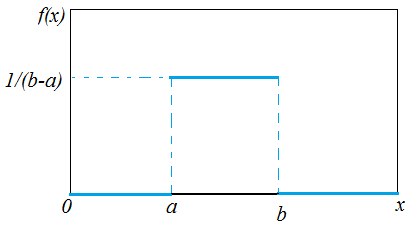
\includegraphics[width=0.5\linewidth,height=0.5\textheight]{uniform} \end{center}

\begin{itemize}
\item
  The cumulative distribution function is
  \[F(x)=\left\{\begin{array}{lll}0& \text{for}& x<a\\
  \frac{x-a}{b-a}& \text{for}& a\leq x <b \\
  1&\text{for}& x \geq b\end{array}\right.\]
\item
  A special case, \(f (x) = 1\) and \(0 \leq x \leq 1\).
\end{itemize}

\hypertarget{exponential-distribution}{%
\subsubsection{Exponential
distribution}\label{exponential-distribution}}

\begin{itemize}
\tightlist
\item
  The exponential density function is
  \[f(x)=\lambda e^{-\lambda x},\; x \geq 0  \;\;\text{and}\;\; \lambda >0\]
\item
  The cumulative distribution function is
  \[F(x)=\int_{-\infty}^x f(u)du =1-e^{-\lambda x}
  \]
\item
  The exponential distribution is often used to model lifetimes or
  waiting times data.
\end{itemize}

\begin{center}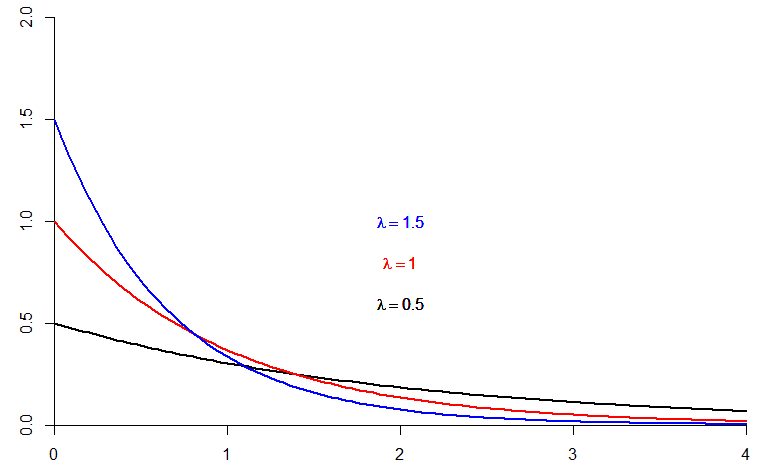
\includegraphics[width=1\linewidth,height=1\textheight]{expdist} \end{center}

\hypertarget{normal-distribution-nmusigma2}{%
\subsubsection{\texorpdfstring{Normal distribution,
\(N(\mu,\sigma^2)\)}{Normal distribution, N(\textbackslash mu,\textbackslash sigma\^{}2)}}\label{normal-distribution-nmusigma2}}

\begin{itemize}
\tightlist
\item
  The normal (Gaussian) distribution plays a central role in probability
  and statistics, probably the most widely known and used of all
  distributions
\item
  The normal distribution fits many natural phenomena, e.g.~human's
  height, weight, IQ scores. In business, for example, the annual cost
  of household insurance, among others.
\item
  The density function of the normal distribution depends on two
  parameters, \(\mu\) and \(\sigma\) (where \(-\infty < \mu < \infty\),
  \(\sigma > 0\)):
  \[f (x) = \frac{1}{\sigma \sqrt{2\pi}} e^{-(x-\mu)^2/2\sigma^2}, -\infty<x<\infty\]
\item
  The parameters \(\mu\) and \(\sigma\) are the mean and standard
  deviation of the normal density.
\item
  We write \(X \sim N(\mu, \sigma^2)\) as short way of saying `\(X\)
  follows a normal distribution with mean \(\mu\) and variance
  \(\sigma^2\)'.
\end{itemize}

\begin{center}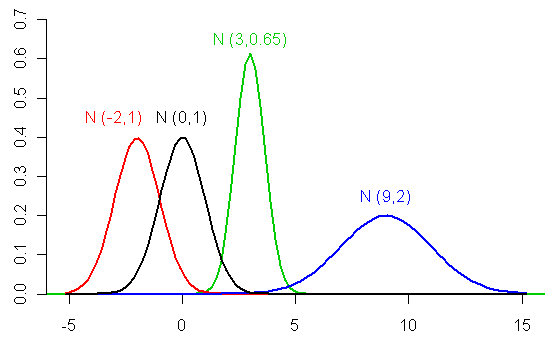
\includegraphics[width=1\linewidth,height=1\textheight]{normdist1} \end{center}

\hypertarget{standard-normal-distribution-nmu0sigma21}{%
\subsubsection{\texorpdfstring{Standard normal distribution
\(N(\mu=0,\sigma^2=1)\)}{Standard normal distribution N(\textbackslash mu=0,\textbackslash sigma\^{}2=1)}}\label{standard-normal-distribution-nmu0sigma21}}

\begin{itemize}
\tightlist
\item
  The probability density function of the standardized normal
  distribution is given by:
\end{itemize}

\[f (z) = \frac{1}{\sqrt{2\pi}} e^{-z^2/2}, -\infty<z<\infty\]

\begin{itemize}
\item
  We write \(Z \sim N(0,1)\) as short way of saying `\(Z\) follows a
  standard normal distribution with mean 0 and variance 1'.
\item
  To standardize any variable \(X\) (into \(Z\)) we calculate \(Z\) as:
  \[ Z = \frac{X - \mu} { \sigma}\] The \(Z\)-score calculated above
  indicates how many standard deviations \(X\) is from the mean.
\end{itemize}

\begin{center}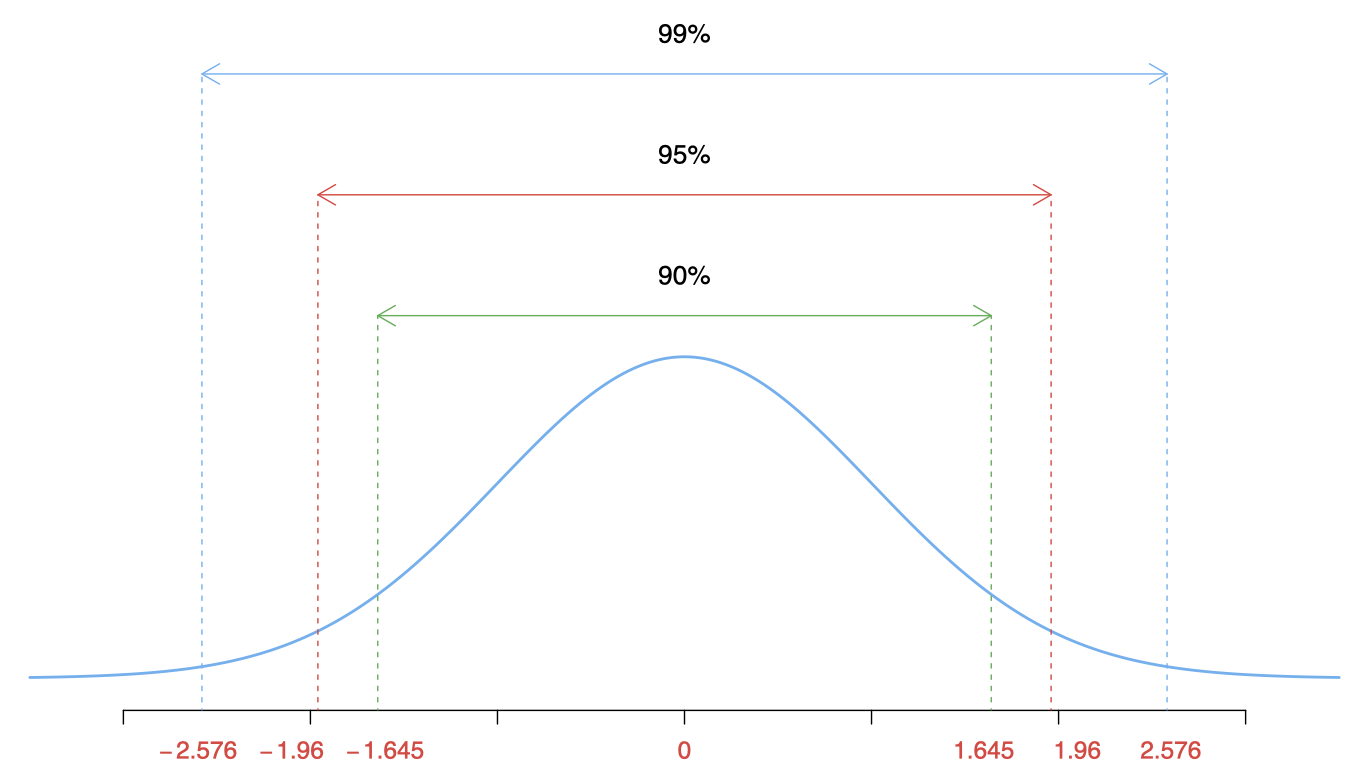
\includegraphics[width=1\linewidth,height=1\textheight]{snormdist2} \end{center}

\hypertarget{log-normal-distribution-and-its-properties}{%
\subsubsection{Log-normal distribution and its
properties}\label{log-normal-distribution-and-its-properties}}

If \(X\sim N(\mu, \sigma^2)\) then \(Y=e^X\) (\(y \geq 0\)) has a
log-normal distribution with mean \(E(Y)=e^{\mu+\sigma^2/2}\) and
variance \(V(Y)=(e^{\sigma^2}-1)e^{2\mu+\sigma^2}\).

\begin{center}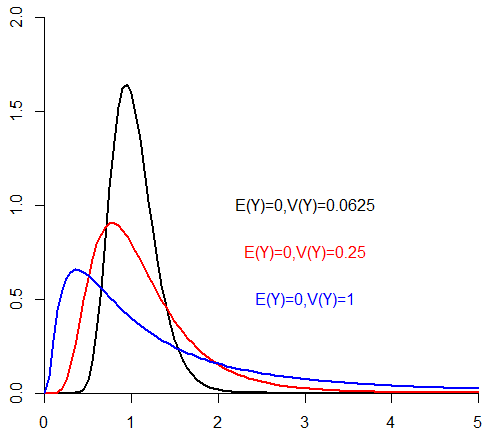
\includegraphics[width=0.8\linewidth,height=0.8\textheight]{lognorm} \end{center}

\hypertarget{distributions-derived-from-the-normal-distribution}{%
\subsubsection{Distributions derived from the normal
distribution}\label{distributions-derived-from-the-normal-distribution}}

We consider here 3 probability distributions derived from the normal
distribution:

\begin{itemize}
\tightlist
\item
  Chi-square distribution
\item
  \(T\) or \(t\) distribution
\item
  \(F\) distribution
\end{itemize}

These distributions are mainly useful for statistical inference,
e.g.~hypothesis testing and confidence intervals (to follow).

\hypertarget{chi-square-distribution-chi2_df}{%
\subsubsection{\texorpdfstring{Chi-square distribution,
\(\chi^2_{(df)}\)}{Chi-square distribution, \textbackslash chi\^{}2\_\{(df)\}}}\label{chi-square-distribution-chi2_df}}

\begin{itemize}
\tightlist
\item
  If \(Z\) is a standard normal random variable, the distribution of
  \(U=Z^2\) is called the chi-square distribution with 1 degree of
  freedom and is denoted by \(\chi^2_1\).
\item
  If \(U_1, U_2,\ldots, U_n\) are independent chi-square random
  variables with 1 degree of freedom, the distribution of
  \(V=U_1+ U_2+\ldots+ U_n\) is called the chi-square distribution with
  \(n\) degrees of freedom and is denoted by \(\chi^2_n\).
\end{itemize}

\begin{center}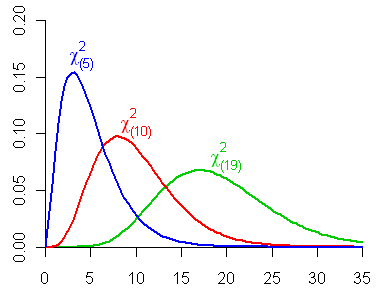
\includegraphics[width=0.8\linewidth,height=0.8\textheight]{chidist} \end{center}

\hypertarget{t-distribution-t_df}{%
\subsubsection{\texorpdfstring{\(T\) distribution,
\(t_{(df)}\)}{T distribution, t\_\{(df)\}}}\label{t-distribution-t_df}}

If \(Z \sim N(0,1)\) and \(U \sim \chi^2_n\) and \(Z\) and \(U\) are
independent, then the distribution of \(Z/\sqrt{U/n}\) is called the
\(t\) distribution with \(n\) degrees of freedom.

\begin{center}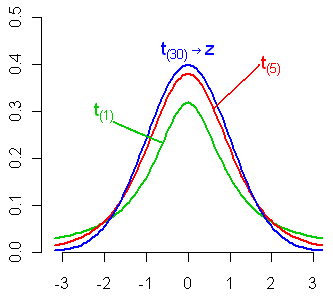
\includegraphics[width=0.8\linewidth,height=0.8\textheight]{tdist} \end{center}

\hypertarget{f-distribution-f_df_1df_2}{%
\subsubsection{\texorpdfstring{\(F\) distribution,
\(F_{(df_1,df_2)}\)}{F distribution, F\_\{(df\_1,df\_2)\}}}\label{f-distribution-f_df_1df_2}}

Let \(U\) and \(V\) be independent chi-square random variables with
\(m\) and \(n\) degrees of freedom, respectively. The distribution of
\[W=\frac{U/m}{V/n}\] is called the \(F\) distribution with \(m\) and
\(n\) degrees of freedom and is denoted by \(F_{m,n}\).

\begin{center}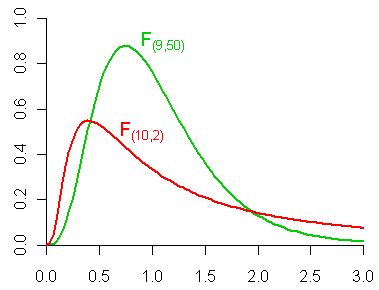
\includegraphics[width=0.5\linewidth,height=0.5\textheight]{fdist} \end{center}

\hypertarget{example}{%
\subsubsection{Example}\label{example}}

\begin{itemize}
\tightlist
\item
  If \(f_X\) is a normal density function with parameters \(\mu\) and
  \(\sigma\), then
\end{itemize}

\[f_Y (y) = \frac{1}{a\sigma\sqrt{2\pi }}exp\left[-\frac{1}{2}\left(\frac{y-b-a\mu}{a\sigma}\right)^2\right]\]

\begin{itemize}
\item
  Thus, \(Y = aX + b\) follows a normal distribution with parameters
  \(a \mu + b\) and \(a\sigma\).
\item
  If \(X \sim N(\mu, \sigma^2)\) and \(Y = aX + b\), then
  \(Y \sim N(a \mu + b, a^2\sigma^2)\).
\item
  Can you use this to show that \(Z\sim N(0,1)\)?
\end{itemize}

\hypertarget{joint-distribution}{%
\subsection{Joint distribution}\label{joint-distribution}}

\begin{itemize}
\tightlist
\item
  The joint behaviour of two random variables, \(X\) and \(Y\), is
  determined by the cumulative distribution function,
  \[F(x,y)=P(X\leq x, Y \leq y)\] regardless of whether \(X\) and \(Y\)
  are continuous or discrete. The cdf gives the probability that the
  point \((X,Y)\) belongs to a semi-infinite rectangle in the plane.
\end{itemize}

\begin{center}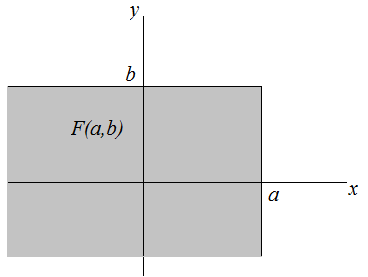
\includegraphics[width=0.5\linewidth,height=0.5\textheight]{joint1} \end{center}

\begin{itemize}
\item
  The joint density function \(f(x,y)\) of two \textbf{continuous random
  variables} \(X\) and \(Y\) is such that \[f(x,y) \geq 0\]
  \[\int_{-\infty}^{\infty}\int_{-\infty}^{\infty}f(x,y)\;dxdy=1\]
  \[\int_{c}^{d}\int_{a}^{b}f(x,y)dxdy=P(a \leq X \leq b, c \leq Y \leq d )\]
  The marginal density function of \(X\) is
  \[f_X(x)=\int_{-\infty}^{\infty}f(x,y)\;dy\] Similarly, the marginal
  density function of \(Y\) is
  \[f_Y(y)=\int_{-\infty}^{\infty}f(x,y)\;dx\]
\item
  The \textbf{cdf} of two \textbf{continuous random variables} \(X\) and
  \(Y\) can be obtained as
  \[F(x,y)=\int_{-\infty}^{x}\int_{-\infty}^{y}f(u,v)dudv\] and
  \[f(x,y)=\frac{\partial^2}{\partial x \partial y}F(x,y)\] wherever the
  derivative is defined.
\end{itemize}

\hypertarget{conditional-probability-density-function-pdf}{%
\subsection{Conditional probability (density) function,
PDF}\label{conditional-probability-density-function-pdf}}

\begin{itemize}
\tightlist
\item
  The conditional probability (density) functions may be obtained as
  follows:
  \[f_{X|Y}(x|y)=\frac{f(x,y)}{f(y)}\;\;\;\text{conditional PDF of $X$}\]
  \[f_{Y|X}(y|x)=\frac{f(x,y)}{f(x)}\;\;\;\text{conditional PDF of $Y$}\]
\item
  Two random variables \(X\) and \(Y\) are statistically independent if
  and only if \[f(x,y)=f(x)f(y)\] That is, if the joint PDF can be
  expressed as the product of the marginal PDFs. So,
  \[f_{X|Y}(x|y)=f(x)\;\;\text{and}\;\;f_{Y|X}(y|x)=f(y)\]
\end{itemize}

\hypertarget{properties-of-expected-values-and-variance}{%
\subsection{Properties of Expected values and
Variance}\label{properties-of-expected-values-and-variance}}

\begin{itemize}
\item
  The expected value of a constant is the constant itself, i.e.~if \(c\)
  is a constant, \(E(c)=c\).
\item
  The variance of a constant is zero, i.e.~if \(c\) is a constant,
  \(Var(c)=0\).
\item
  If \(a\) and \(b\) are constants, and \(Y = aX + b\), then
  \(E(Y)=a E(X)+b\) and \(Var(Y) = a^2Var(X)\) (if \(Var(X)\) exists).
\item
  If \(X\) and \(Y\) are independent, then \(E(XY) = E(X)E(Y)\) and
  \[Var(X+ Y)=Var(X) + Var(Y)\] \[Var(X- Y)=Var(X) + Var(Y)\]
\item
  If \(X\) and \(Y\) are independent random variables and \(g\) and
  \(h\) are fixed functions, then \[E[g(X)h(Y )] = E[g(X)]E[h(Y )]\]
\end{itemize}

\hypertarget{covariance}{%
\subsection{Covariance}\label{covariance}}

\begin{itemize}
\tightlist
\item
  Let \(X\) and \(Y\) be two random variables with means \(\mu_x\) and
  \(\mu_y\), respectively. Then the \textbf{covariance} between the two
  variables is defined as
  \[cov(X,Y)=E\left\{(X-\mu_x)(Y-\mu_y)\right\}=E(XY)-\mu_x\mu_y\]
\item
  If \(X\) and \(Y\) are independent, then \(cov(X,Y)=0\).
\item
  If two variables are uncorrelated, that does not in general imply that
  they are independent.
\item
  \(Var(X)=cov(X,X)\)
\item
  \(cov(bX+a, dY+c)=bd\; cov(X,Y)\), where \(a,b,c\), and \(d\) are
  constants.
\end{itemize}

\hypertarget{correlation-coefficient}{%
\subsection{Correlation Coefficient}\label{correlation-coefficient}}

\begin{itemize}
\tightlist
\item
  The (population) correlation coefficient \(\rho\) is defined as
  \[\rho=\frac{cov(X,Y)}{\sqrt{Var(X)Var(Y)}}=\frac{cov(X,Y)}{\sigma_x \sigma_y}\]
\item
  Thus, \(\rho\) is a measure of \textbf{linear} association between two
  variables and lies between \(-1\) (indicating perfect negative
  association) and \(+1\) (indicating perfect positive association).
\item
  \(cov(X,Y)=\rho \;\sigma_x \sigma_y\)
\item
  Variances of correlated variables,
  \[Var(X\pm Y)=Var(X)+Var(Y) \pm 2 cov(X,Y)\]
  \[Var(X\pm Y)=Var(X)+Var(Y) \pm 2 \rho\; \sigma_x \sigma_y\]
\end{itemize}

\hypertarget{conditional-expectation-and-conditional-variance}{%
\subsection{Conditional expectation and conditional
variance}\label{conditional-expectation-and-conditional-variance}}

Let \(f(x,y)\) be the joint PDF of random variables \(X\) and \(Y\). The
conditional expectation of \(X\), given \(Y=y\), is defined as
\[E(X|Y=y)=\sum_x x f_{X|Y}(x|Y=y)\;\;\; \text{if $X$ is discrete}\]
\[E(X|Y=y)=\int_{-\infty}^{\infty} x f_{X|Y}(x|Y=y)dx\;\;\; \text{if $X$ is continuous}\]
The conditional variance of \(X\) given \(Y=y\) is defined as, if \(X\)
is discrete, \[Var(X|Y=y)=\sum_x [X-E(X|Y=y)]^2 f_{X|Y}(x|Y=y)\] and if
\(X\) is continuous,
\[Var(X|Y=y)=\int_{-\infty}^{\infty} [X-E(X|Y=y)]^2 f_{X|Y}(x|Y=y)dx\]

\pagebreak

\hypertarget{sampling}{%
\section{Sampling}\label{sampling}}

\hypertarget{sampling-1}{%
\subsection{Sampling}\label{sampling-1}}

\begin{itemize}
\tightlist
\item
  Sampling is widely used as a means of gathering useful information
  about a population.
\item
  Data are gathered from samples and conclusions are drawn about the
  population as a part of the inferential statistics process.
\item
  Often, a sample provides a reasonable means for gathering such useful
  decision-making information that might be otherwise unattainable and
  unaffordable.
\item
  Sampling error occurs when the sample is not representative of the
  population.
\end{itemize}

\hypertarget{random-versus-non-random-sampling}{%
\subsection{Random versus non-random
sampling}\label{random-versus-non-random-sampling}}

\begin{itemize}
\item
  In \textbf{random sampling} every unit of the population has the same
  probability of being selected into the sample.

  \begin{itemize}
  \tightlist
  \item
    Simple random sampling
  \item
    Stratified sampling
  \item
    Cluster sampling
  \item
    Multistage sampling
  \end{itemize}
\item
  In \textbf{non-random sampling} not every unit of the population has
  the same probability of being selected into the sample.

  \begin{itemize}
  \tightlist
  \item
    Convenience sampling
  \item
    Judgement sampling
  \item
    Quota sampling
  \end{itemize}
\end{itemize}

\hypertarget{simple-random-sampling}{%
\subsection{Simple random sampling}\label{simple-random-sampling}}

\textbf{Simple random sampling:} is the basic sampling technique where
we select a group of subjects (a sample) from a larger group (a
population). Each individual is chosen entirely by chance and each
member of the population has an equal chance of being included in the
sample.

\hypertarget{central-limit-theorem}{%
\subsection{Central limit theorem}\label{central-limit-theorem}}

Let \(X_1, X_2, \ldots\) be independent and identically distributed
(i.i.d.) random variables with mean \(\mu\) and variance \(\sigma^2\).
Then as \(n\) increases indefinitely (i.e.~\(n\rightarrow\infty\)),
\(\overline{X}_n=\sum_{i=1}^{n}X_i/n\) approaches the normal
distribution with mean \(\mu\) and variance \(\sigma^2/n\). That is
\[\overline{X}_n \underset{n\rightarrow\infty}{\sim} N(\mu, \sigma^2/n)\]

Note that this result holds true regardless of the form of the
underlying distribution. As a result, it follows that
\[Z=\frac{\overline{X}_n-\mu}{\sigma/\sqrt{n}}\underset{n\rightarrow\infty}{\sim} N(0,1)\]
That is, \(Z\) is a standardized normal variable.
 
\hypertarget{sampling-distribution-of-the-sample-mean-barx}{%
\subsection{\texorpdfstring{Sampling distribution of the sample mean
\(\bar{x}\)}{Sampling distribution of the sample mean \textbackslash bar\{x\}}}\label{sampling-distribution-of-the-sample-mean-barx}}

The sampling distribution of a statistic is the probability distribution
of that statistic.

\begin{center}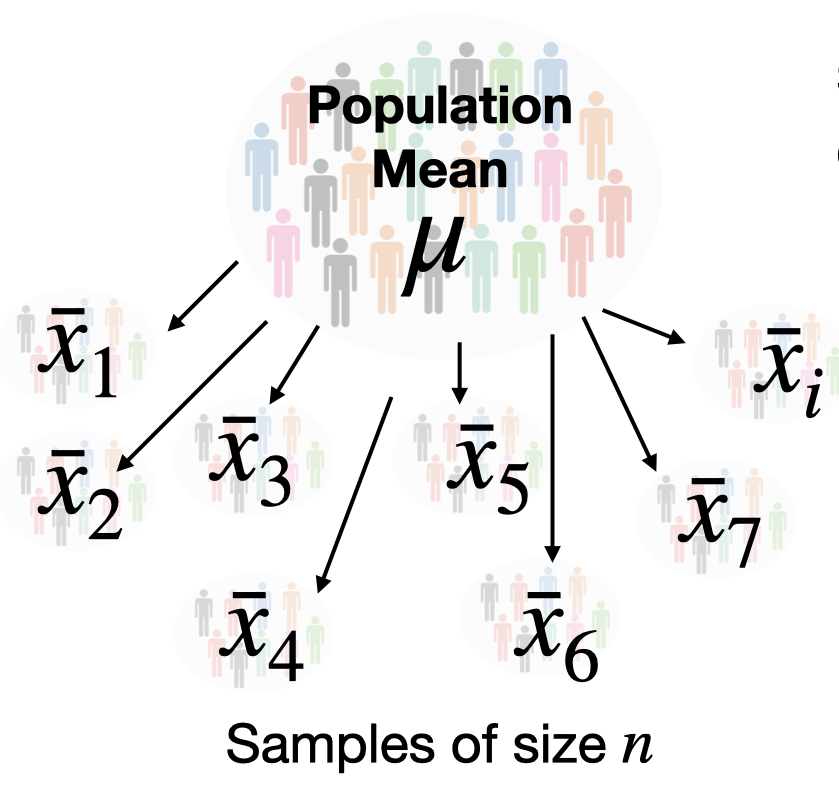
\includegraphics[width=0.8\linewidth,height=0.8\textheight]{stat4} \end{center}

There are two cases:

\begin{enumerate}
\def\labelenumi{\arabic{enumi}.}
\item
  Sampling is from a normally distributed population with a known
  population variance:
  \[\bar{x}\sim N\left(\mu, \frac{\sigma^2}{n}\right) \] That is, the
  sampling distribution of the sample mean is normal with mean
  \(\mu_{\bar{x}}=\mu\) and standard deviation
  \(\sigma_{\bar{x}}=\sigma/\sqrt{n}\).
\item
  Sampling is from a non-normally distributed population with known
  population variance and \(n\) is large, then the mean of \(\bar{x}\),
  \[\mu_{\bar{x}}=\mu\] and the variance,
  \[\sigma^2_{\bar{x}}=\left\{\begin{array}{ll}
  \frac{\sigma^2}{n} & \text{with replacement (infinite  population)}\\
  &\\
  \frac{\sigma^2}{n}\frac{N-n}{N-1} & \text{without replacement (finite  population)}
  \end{array}\right.\]
\end{enumerate}

\begin{itemize}
\item
  If the sample size is large, the central limit theorem applies and the
  sampling distribution of \(\bar{x}\) will be approximately normal.
\item
  The standard deviation of the sampling distribution of the sample
  mean, \(\sigma_{\bar{x}}\), is called the \textbf{standard error} of
  the mean or, simply, the standard error
\item
  If \(\bar{x}\) is a normal distributed (or approximately normal
  distributed), we can use the following formula to transform
  \(\bar{x}\) to a \(Z\)-score.
\end{itemize}

\[Z=\frac{\bar{x}-\mu_{\bar{x}}}{\sigma_{\bar{x}}}\] where
\(Z \sim N(0,1)\).

\hypertarget{sampling-distribution-of-the-sample-proportion}{%
\subsection{Sampling distribution of the sample
proportion}\label{sampling-distribution-of-the-sample-proportion}}

\begin{itemize}
\item
  When the sample size \textbf{\(n\) is large}, the distribution of the
  sample proportion, \(\hat{\pi}\), is approximately normally
  distributed by the use of the central limit theorem,
  \[\hat{\pi}\thickapprox N\left(\pi,\frac{\pi(1-\pi)}{n}\right)\] then
  \[Z=\frac{\hat{\pi}-\pi}{\sqrt{\frac{\pi(1-\pi)}{n}}}\thickapprox N(0,1)\]
  where \(\hat{\pi}=x/n\), \(x\) is the number in the sample with the
  characteristic of interest.
\item
  A widely used criterion is that both \(n\pi\) and \(n(1-\pi)\) must be
  greater than 5 for this approximation to be reasonable.
\end{itemize}

\hypertarget{sampling-distribution-of-the-sample-variance}{%
\subsection{Sampling distribution of the sample
variance}\label{sampling-distribution-of-the-sample-variance}}

Sampling is from a normally distributed population with mean \(\mu\) and
variance \(\sigma^2\). The sample variance is
\[s^2=\frac{1}{n-1}\sum_{i=1}^{n} (x_i-\bar{x})^2\] and
\[E(s^2)=\sigma^2\] \[Var(s^2)= 2\sigma^4/(n-1)\] Then
\[\frac{(n-1)s^2}{\sigma^2}\sim \chi^2_{n-1}\]

\hypertarget{example-1}{%
\subsection{Example}\label{example-1}}

Suppose that during any hour in a large department store, the average
number of shoppers is 448, with a standard deviation of 21 shoppers.
What is the probability that a random sample of 49 different shopping
hours will yield a sample mean between 441 and 446 shoppers?

\[\mu =448, \sigma=21, n=49\] \begin{align*}
P(441\leq \bar{x} \leq 446)=&\left(
\frac{441-448}{21/\sqrt{49}}\leq \frac{\bar{x}-\mu}{\sigma/\sqrt{n}}\leq \frac{446-448}{21/\sqrt{49}}\right)\\
P(-2.33 \leq Z \leq -0.67)=&P(Z \leq -0.67)-P(Z \leq -2.33)\\
=&0.2514-0.0099=0.2415 
\end{align*}

\begin{center}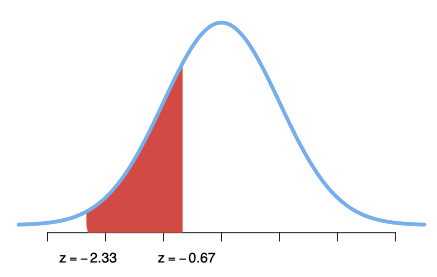
\includegraphics[width=0.8\linewidth,height=0.8\textheight]{ex.sampling} \end{center}

That is there is a 24.15\% chance of randomly selecting 49 hourly
periods for which the sample mean is between 441 and 446 shoppers.

We used the standard normal table to obtain these probabilities. We can
also use R.

%\begin{Shaded}
\begin{Highlighting}[]
\FunctionTok{pnorm}\NormalTok{(}\SpecialCharTok{{-}}\FloatTok{0.67}\NormalTok{)}\SpecialCharTok{{-}}\FunctionTok{pnorm}\NormalTok{(}\SpecialCharTok{{-}}\FloatTok{2.33}\NormalTok{)}
\end{Highlighting}
%\end{Shaded}

\begin{verbatim}
## [1] 0.2415258
\end{verbatim}

\pagebreak

\hypertarget{estimation}{%
\section{Estimation}\label{estimation}}

\hypertarget{estimation-1}{%
\subsection{Estimation}\label{estimation-1}}

\begin{itemize}
\tightlist
\item
  The values of population parameters are often unknown.
\item
  We use a representative sample of the population to estimate the
  population parameters.
\end{itemize}

There are two types of estimation:

\begin{itemize}
\tightlist
\item
  Point Estimation
\item
  Interval Estimation
\end{itemize}

\begin{center}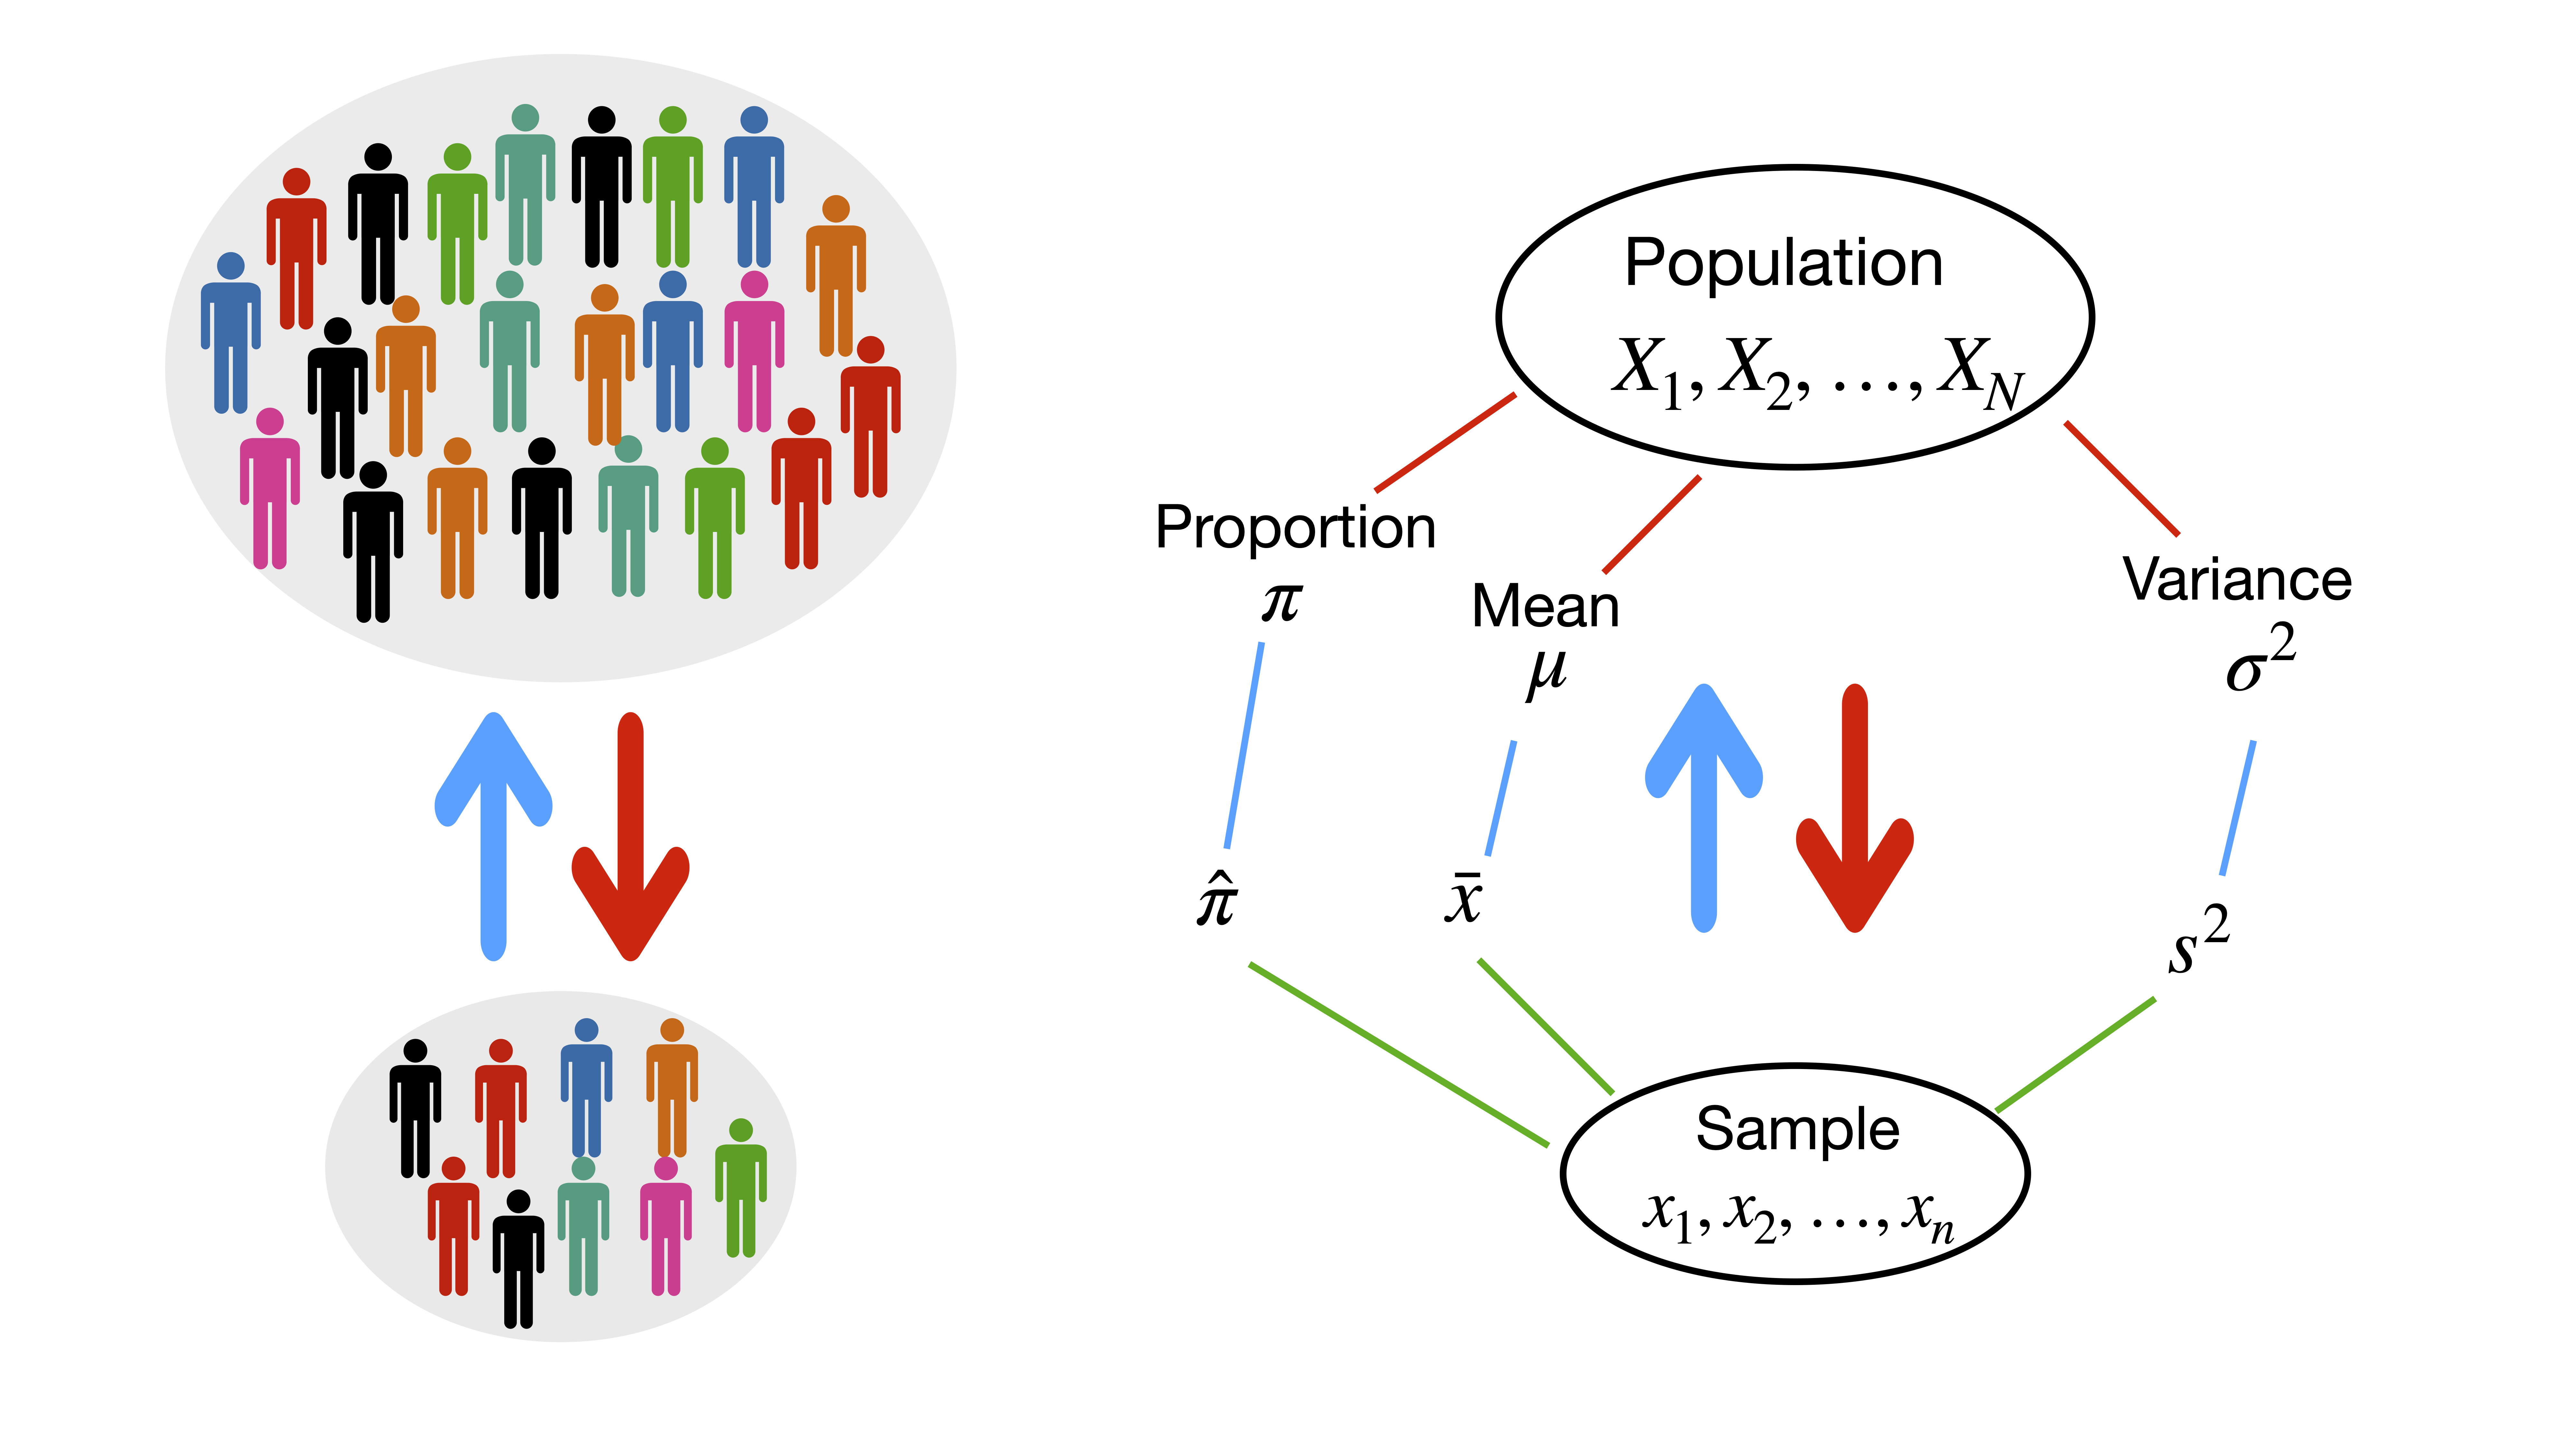
\includegraphics[width=1\linewidth,height=1\textheight]{stat1new} \end{center}

\hypertarget{point-estimation}{%
\subsection{Point estimation}\label{point-estimation}}

\begin{itemize}
\item
  A \textbf{point estimate} is a single numerical value used to estimate
  the corresponding population parameter. A point estimate is obtained
  by selecting a suitable \textbf{statistic} (a suitable function of the
  data) and computing its value from the given sample data. The selected
  statistic is called the \textbf{point estimator}.
\item
  The point estimator is a random variable, so it has a distribution,
  mean, variance etc.
\item
  e.g.~the sample mean \(\overline{X}=(1/n)\sum_{i=1}^{n}X_i\) is one
  possible point \{\bf estimator\} of the population mean \(\mu\), and
  the point \textbf{estimate} is \(\bar{x}=(1/n)\sum_{i=1}^{n}x_i\).
\end{itemize}

\textbf{Properties:}

\begin{itemize}
\item
  Let \(\theta\) be the unknown population parameter and
  \(\hat{\theta}\) be its estimator. The parameter space is denoted by
  \(\Theta\).
\item
  An estimator \(\hat{\theta}\) is called \textbf{unbiased estimator} of
  \(\theta\) if \(E( \hat{\theta}) = \theta\).
\item
  The bias of the estimator \(\hat{\theta}\) is defined as
  \(Bias(\hat{\theta})=E(\hat{\theta})-\theta\)
\item
  \textbf{Mean Square Error (MSE)} is a measure of how close
  \(\hat{\theta}\) is, on average, to the true \(\theta\),
  \[MSE=E[(\hat{\theta}-\theta)^2]= Var(\hat{\theta}) + [Bias (\hat{\theta})]^2\]
\end{itemize}

\hypertarget{interval-estimation}{%
\subsection{Interval estimation}\label{interval-estimation}}

\begin{itemize}
\item
  An \textbf{interval estimate (confidence interval)} is an interval, or
  range of values, used to estimate a population parameter.
\item
  The \textbf{level of confidence} \((1-\alpha)100\%\) is the
  probability that the interval estimate contains the population
  parameter.
\item
  Interval estimate components:
\end{itemize}

\[\text{point estimate}\; \pm \; (\text{critical value}\; \times\; \text{standard error})\]

\hypertarget{confidence-intervals-for-the-population-mean}{%
\subsection{Confidence intervals for the population
mean}\label{confidence-intervals-for-the-population-mean}}

\begin{itemize}
\item
  When sampling is from a normal distribution with known variance
  \(\sigma^2\), then a \(100(1-\alpha)\%\) confidence interval for the
  population mean \(\mu\) is
  \[ \bar{x}\pm z_{\alpha/2} \; (\sigma/\sqrt{n} )\] where
  \(z_{\alpha/2}\) can be obtained from the standard normal distribution
  table.

  \begin{longtable}[]{@{}lcr@{}}
  \toprule()
  \(100(1-\alpha)\%\) & \(\alpha\) & \(z_{\alpha/2}\) \\
  \midrule()
  \endhead
  \(90\%\) & 0.10 & 1.645 \\
  \(95\%\) & 0.05 & 1.96 \\
  \(99\%\) & 0.01 & 2.58 \\
  \bottomrule()
  \end{longtable}
\item
  If \(\sigma\) is unknown and \(n \geq 30\), the sample standard
  deviation \(s=\sqrt{\sum(x_i-\bar{x})^2/(n-1)}\) can be used in place
  of \(\sigma\).
\end{itemize}

\begin{center}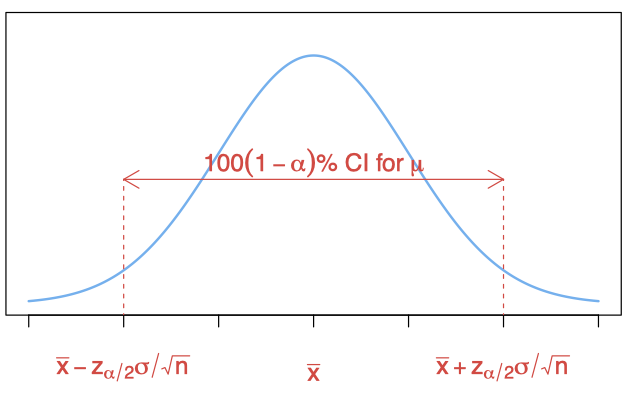
\includegraphics[width=1\linewidth,height=1\textheight]{estimationmean} \end{center}

\begin{center}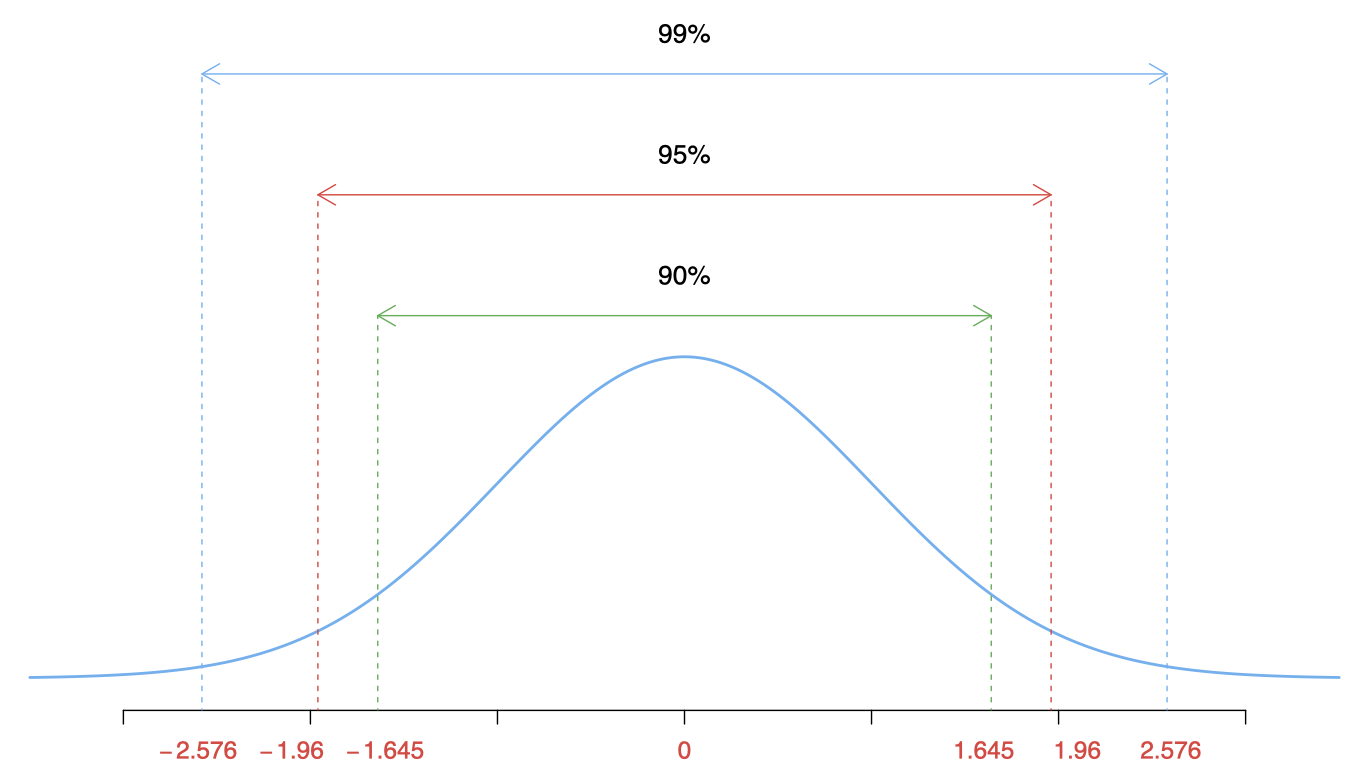
\includegraphics[width=1\linewidth,height=1\textheight]{snormdist2} \end{center}

\begin{itemize}
\item
  If the sampling is from a non-normal distribution and \(n \geq 30\),
  then the sampling distribution of \(\bar{x}\) is approximately
  normally distributed (central limit theorem) and we can use the same
  formula, \(\bar{x}\pm z_{\alpha /2} \; (\sigma /\sqrt{n} )\), to
  construct the approximate confidence interval for population mean.
\item
  When sampling is from a normal distribution whose standard deviation
  \(\sigma\) is unknown and the sample size is small, the
  \(100(1-\alpha)\%\) confidence interval for the population mean
  \(\mu\) is \[ \bar{x}\pm t_{\alpha /2} \; (s /\sqrt{n} )\] where
  \(t_{\alpha/2}\) can be obtained from the \(t\) distribution table
  with \(df=n-1\) and \(s\) is the sample standard deviation which is
  given by \[s=\sqrt{\frac{\sum(x_i-\bar{x})^2}{n-1}}\]
\item
  If \(\sigma\) is unknown, and we neither have normal population nor
  large sample, then we should use nonparametric statistics (not cover
  in this course).
\end{itemize}

\hypertarget{interpreting-confidence-intervals}{%
\subsection{Interpreting confidence
intervals}\label{interpreting-confidence-intervals}}

\begin{itemize}
\item
  \textbf{Probabilistic interpretation:} In repeated sampling, from some
  population, \(100(1-\alpha)\%\) of all intervals which we constructed
  will in the long run include the population parameter.
\item
  \textbf{Practical interpretation:} When sampling is from some
  population, we have \(100(1-\alpha)\%\) confidence that the single
  computed interval contains the population parameter.
\end{itemize}

\hypertarget{confidence-interval-for-a-population-proportion}{%
\subsection{Confidence interval for a population
proportion}\label{confidence-interval-for-a-population-proportion}}

The \(100(1-\alpha)\%\) confidence interval for a population proportion
\(\pi\) is given by
\[\hat{\pi}\pm z_{\alpha/2} \sqrt{\frac{\hat{\pi}(1-\hat{\pi})}{n}} \]
where \(\hat{\pi}\) is the sample proportion.

\hypertarget{confidence-interval-for-a-population-variance}{%
\subsection{Confidence interval for a population
variance}\label{confidence-interval-for-a-population-variance}}

The \(100(1-\alpha)\%\) confidence interval for the variance,
\(\sigma^2\), of \textbf{a normally distributed} population is given by
\[\left(\frac{(n-1)s^2}{\chi^2_{\frac{\alpha}{2}, n-1}}, \frac{(n-1)s^2}{\chi^2_{1-\frac{\alpha}{2}, n-1}}\right)\]
where \(s^2=\frac{1}{n-1}\sum_{i=1}^{n}(x_i-\bar{x})^2\) is the sample
variance.

\begin{center}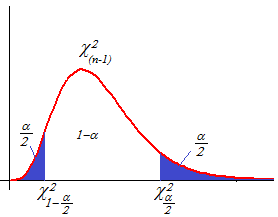
\includegraphics[width=1\linewidth,height=1\textheight]{chidist1} \end{center}

\hypertarget{example-2}{%
\subsection{Example}\label{example-2}}

Suppose a car rental firm wants to estimate the average number of
kilometres travelled per day by each of its cars rented in London. A
random sample of 20 cars rented in London reveals that the sample mean
travel distance per day is 85.5 kilometres, with a population standard
deviation of 19.3 kilometres. Compute a 99\% confidence interval to
estimate \(\mu\).

For a 99\% level of confidence, a \(z\) value of 2.58 is obtained (from
the standard normal table). Assume that number of kilometres travelled
per day is normally distributed.\% in the population.
\[\bar{x}\pm z_{\alpha/2} \frac{\sigma}{\sqrt{n}}\]
\[85.5 \pm 2.58 \frac{19.3}{\sqrt{20}}\] \[85.5 \pm 11.1\]
\[\text{thus}\;\; 74.4 \leq \mu \leq 96.6\]

%\begin{Shaded}
\begin{Highlighting}[]
\FunctionTok{qnorm}\NormalTok{((}\DecValTok{1}\FloatTok{{-}0.99}\NormalTok{)}\SpecialCharTok{/}\DecValTok{2}\NormalTok{)}
\end{Highlighting}
%\end{Shaded}

\begin{verbatim}
## [1] -2.575829
\end{verbatim}

\pagebreak

\hypertarget{hypothesis-testing-one-sample}{%
\section{Hypothesis Testing One
Sample}\label{hypothesis-testing-one-sample}}

\hypertarget{hypothesis-testing-motivation}{%
\subsection{Hypothesis testing:
Motivation}\label{hypothesis-testing-motivation}}

We often encounter such statements or claims:

\begin{itemize}
\item
  A newspaper claims that the average starting salary of MBA graduates
  is over \pounds50K. (one sample test)
\item
  A claim about the efficiency of a particular diet program, the average
  weight after the program is less than the average weight before the
  program. (two paired samples test)
\item
  On average female managers earn less than male managers, given that
  they have the same qualifications and skills. (two independent samples
  test)
\end{itemize}

So we have claims about the populations' means (averages) and we would
like to verify or examine these claims.

This is a kind of problem that \textbf{hypothesis testing} is designed
to solve.

\hypertarget{the-nature-of-hypothesis-testing}{%
\subsection{The nature of hypothesis
testing}\label{the-nature-of-hypothesis-testing}}

\begin{itemize}
\item
  We often use inferential statistics to make decisions or judgments
  about the value of a parameter, such as a population mean.
\item
  Typically, a hypothesis test involves two hypotheses:

  \begin{itemize}
  \tightlist
  \item
    \textbf{Null hypothesis:} a hypothesis to be tested, denoted by
    \(H_0\).
  \item
    \textbf{Alternative hypothesis (or research hypothesis):} a
    hypothesis to be considered as an alternate to the null hypothesis,
    denoted by \(H_1\) or \(H_a\).
  \end{itemize}
\item
  The problem in a hypothesis test is to decide whether or not the null
  hypothesis should be rejected in favour of the alternative hypothesis.
\item
  The choice of the alternative hypothesis should reflect the purpose of
  performing the hypothesis test.
\item
  How do we decide whether or not to reject the null hypothesis in
  favour of the alternative hypothesis?
\item
  Very roughly, the procedure for deciding is the following:

  \begin{itemize}
  \tightlist
  \item
    Take a random sample from the population.
  \item
    If the sample data are consistent with the null hypothesis, then do
    not reject the null hypothesis; if the sample data are inconsistent
    with the null hypothesis, then reject the null hypothesis and
    conclude that the alternative hypothesis is true.
  \end{itemize}
\item
  \textbf{Test statistic:} the statistic used as a basis for deciding
  whether the null hypothesis should be rejected.
\item
  The \textbf{test statistic} is a random variable which therefore has a
  sampling distribution with mean and standard deviation (so-called
  \textbf{standard error}).
\end{itemize}

\hypertarget{type-i-and-type-ii-errors}{%
\subsection{Type I and Type II Errors}\label{type-i-and-type-ii-errors}}

\begin{center}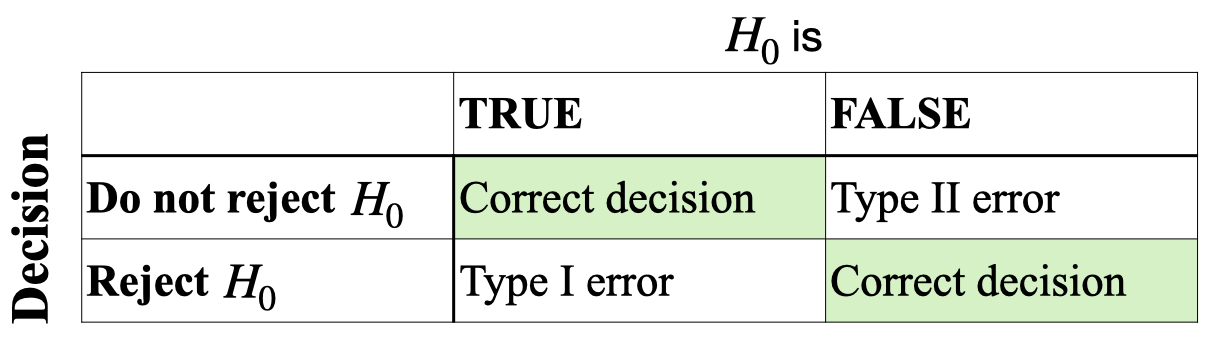
\includegraphics[width=1\linewidth,height=0.8\textheight]{hypotab1} \end{center}

\begin{itemize}
\item
  \textbf{Type I error:} rejecting the null hypothesis when it is in
  fact true.
\item
  \textbf{Type II error:} not rejecting the null hypothesis when it is
  fact false.
\item
  The \textbf{significance level}, \(\alpha\), of a hypothesis test is
  defined as the probability of making a Type I error, that is, the
  probability of rejecting a true null hypothesis.
\item
  \textbf{Relation between Type I and II error probabilities:} For a
  fixed sample size, the smaller the Type I error probability,
  \(\alpha\), of rejecting a true null hypothesis, the larger the Type
  II error probability of not rejecting a false null hypothesis and vice
  versa.
\item
  \textbf{Possible conclusions for a hypothesis test:} If the null
  hypothesis is rejected, we conclude that the alternative hypothesis is
  probably true. If the null hypothesis is not rejected, we conclude
  that the data do not provide sufficient evidence to support the
  alternative hypothesis.
\item
  When the null hypothesis is rejected in a hypothesis test performed at
  the significance level \(\alpha\), we say that the results are
  statistically significant at level \(\alpha\).
\end{itemize}

\hypertarget{hypothesis-tests-for-one-population-mean}{%
\subsection{Hypothesis tests for one population
mean}\label{hypothesis-tests-for-one-population-mean}}

In order to test the hypothesis that the population mean \(\mu\) is
equal to a particular value \(\mu_0\), we are going to test the null
hypothesis

\[H_0:\mu=\mu_0\]

against one of the following alternatives:

\begin{itemize}
\tightlist
\item
  \(H_1:\mu\neq\mu_0\) (Two-tailed)
\item
  \(H_1:\mu<\mu_0\) (Left-tailed)
\item
  \(H_1:\mu>\mu_0\) (Right-tailed)
\end{itemize}

In order to test \(H_0\), we need to use one of the following test
statistics, we should choose the one that satisfies the assumptions.

\begin{itemize}
\tightlist
\item
  If \(\sigma\) is known, and we have a normally distributed population
  or large sample (\(n\geq 30\)), then the test statistic, so-called
  \(z\)-test, is \[z=\frac{\bar{x}-\mu_0}{\sigma / \sqrt{n}}\] where
  \(\sigma\) is the standard deviation of the population.
\item
  If \(\sigma\) is unknown, and we have a normally distributed
  population or large sample (\(n \geq 30\)), then the test statistic,
  so-called \(t\)-test, is
  \[t=\frac{\bar{x}-\mu_0}{s/\sqrt{n}}\;\;\text{with}\;\; df=n-1.\]
  where \(s\) is the standard deviation of the sample.
\end{itemize}

\hypertarget{the-p-value-approach-to-hypothesis-testing}{%
\subsection{\texorpdfstring{The \(p\)-value approach to hypothesis
testing}{The p-value approach to hypothesis testing}}\label{the-p-value-approach-to-hypothesis-testing}}

\begin{itemize}
\item
  The \(p\text{-value}\) is the smallest significance level at which the
  null hypothesis would be rejected. The \(p\)-value is also known as
  the observed significance level.
\item
  The \(p\text{-value}\) measures how well the observed sample agrees
  with the null hypothesis. A small \(p\text{-value}\) (close to zero)
  indicates that the sample is not consistent with the null hypothesis
  and the null hypothesis should be rejected. On the other hand, a large
  \(p\text{-value}\) (larger than 0.10) generally indicates a reasonable
  level of agreement between the sample and the null hypothesis.
\item
  As a rule of thumb, if \(p \text{-value} \leq \alpha\) then reject
  \(H_0\); otherwise do not reject \(H_0\).
\end{itemize}

\hypertarget{critical-value-approach-to-hypothesis-testing}{%
\subsection{Critical-value approach to hypothesis
testing}\label{critical-value-approach-to-hypothesis-testing}}

\begin{center}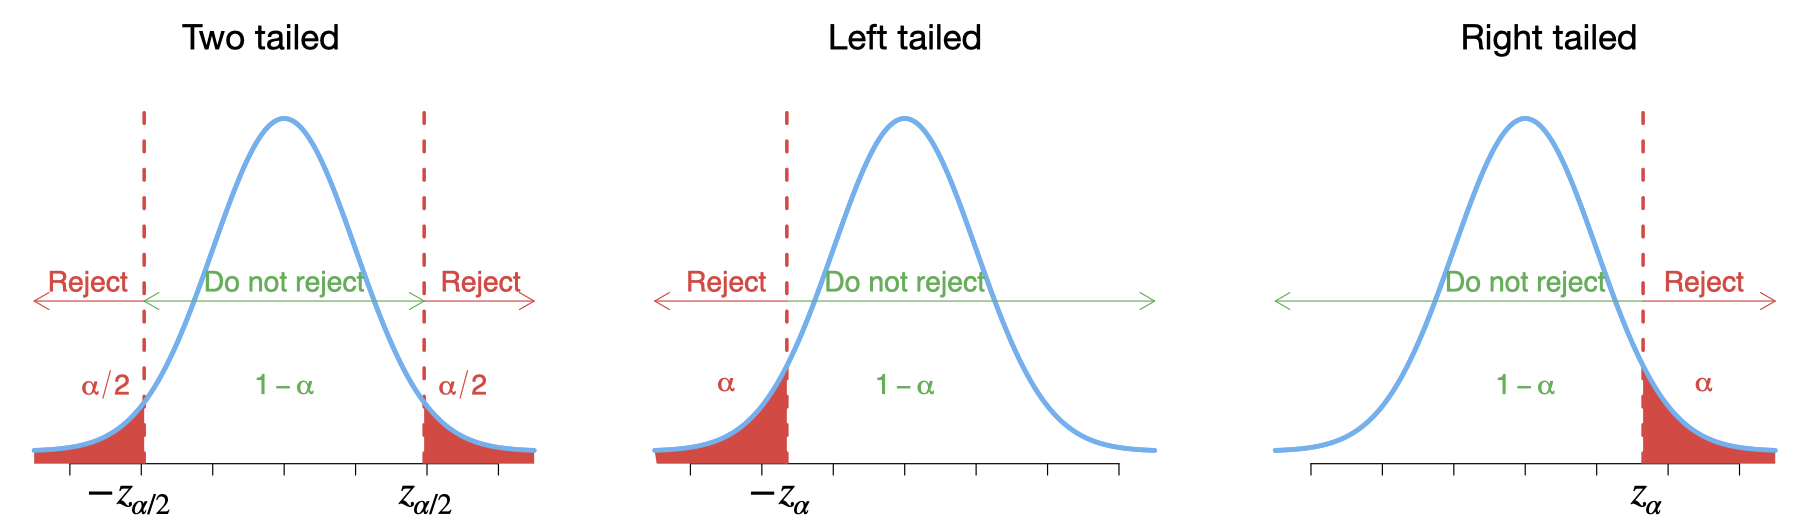
\includegraphics[width=1.3\linewidth,height=1\textheight]{hypoztest} \end{center}

For any specific significance level \(\alpha\), one can obtain these
critical values \(\pm z_{\alpha/2}\) and \(\pm z_{\alpha}\) from the
standard normal table.

\begin{longtable}[]{@{}ccccc@{}}
\toprule()
1.282 & 1.645 & 1.960 & 2.326 & 2.576 \\
\midrule()
\endhead
\(z_{0.10}\) & \(z_{0.05}\) & \(z_{0.025}\) & \(z_{0.01}\) &
\(z_{0.005}\) \\
\bottomrule()
\end{longtable}

If the value of the test statistic falls in the rejection region, reject
\(H_0\); otherwise do not reject \(H_0\).

\begin{center}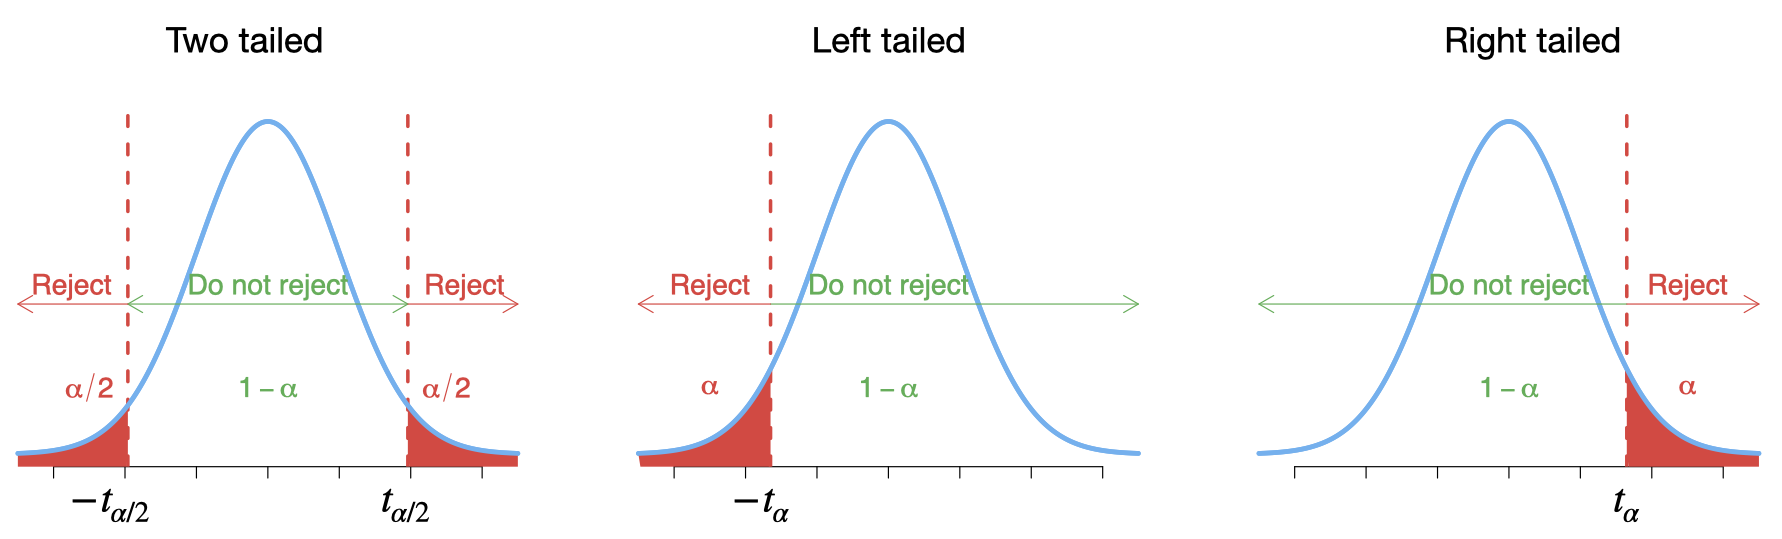
\includegraphics[width=1.3\linewidth,height=0.8\textheight]{hypottest} \end{center}

For any specific significance level \(\alpha\), one can obtain these
critical values \(\pm t_{\alpha/2}\) and \(\pm t_{\alpha}\) from the T
distribution table. For example, for \(df=9\) and \(\alpha=.05\), the
critical values are \(\pm t_{0.025}=\pm 2.262\) and
\(\pm t_{0.05}=\pm 1.833\).

\hypertarget{hypothesis-testing-and-confidence-intervals}{%
\subsection{Hypothesis testing and confidence
intervals}\label{hypothesis-testing-and-confidence-intervals}}

Hypothesis tests and confidence intervals are closely related. Consider,
for instance, a two tailed hypothesis test for a population mean at the
significance level \(\alpha\). It can be shown that the null hypothesis
will be rejected if and only if the value \(\mu_0\) given for the mean
in the null hypothesis lies outside the 100(\(1-\alpha\))-level
confidence interval for \(\mu\).

\textbf{Example:}

\begin{itemize}
\tightlist
\item
  At significance level \(\alpha=0.05\), we want to test
  \(H_0: \mu = 40\) against \(H_1: \mu \neq 40\) (so here \(\mu_0=40\)).
\item
  Suppose that the 95\% confidence interval for \(\mu\) is
  \(35<\hspace{-1mm}\mu\hspace{-1mm}<38\).
\item
  As \(\mu_0=40\) lies outside this confidence intervals, we reject
  \(H_0\).
\end{itemize}

\hypertarget{test-of-normality}{%
\subsection{Test of Normality}\label{test-of-normality}}

One of the assumptions in order to use \(z\)-test or \(t\)-test is that
the population which we sampled from is normally distributed. However we
did not yet test this assumption, we should perform a so-called
\textbf{test of normality}. In order to do so:

\begin{itemize}
\item
  We can plot our data sample, e.g.~histogram, boxplot, stem-and-leaf
  and normal Q-Q plot
\item
  Use normality tests such as Kolmogorov-Smirnov test or Shapiro-Wilk
  test. The null and alternative hypotheses are:

  \begin{itemize}
  \tightlist
  \item
    \(H_0\): the population being sampled is normally distributed.
  \item
    \(H_1\): the population being sampled is nonnormally distributed.
  \end{itemize}
\end{itemize}

If \(\sigma\) is unknown, and we neither have normal population nor
large sample, then we should use nonparametric tests instead of
\(z\)-test or \(t\)-test (not cover in this course).

\hypertarget{example-3}{%
\subsection{Example}\label{example-3}}

A company reported that a new car model equipped with an enhanced manual
transmission averaged 29 mpg on the highway. Suppose the Environmental
Protection Agency tested 15 of the cars and obtained the following gas
mileages.

\begin{longtable}[]{@{}ccccc@{}}
\toprule()
\endhead
27.3 & 30.9 & 25.9 & 31.2 & 29.7 \\
28.8 & 29.4 & 28.5 & 28.9 & 31.6 \\
27.8 & 27.8 & 28.6 & 27.3 & 27.6 \\
\bottomrule()
\end{longtable}

What decision would you make regarding the company's claim on the gas
mileage of the car? Perform the required hypothesis test at the 5\%
significance level.

\textbf{Solution:}

The null and alternative hypotheses:
\[H_0: \mu =29 \;\text{mpg vs.}\;\;\; H_1: \mu \neq 29\; \text{mpg} \]
The value of the test statistic,
\[ t=\frac{\bar{x}-\mu _{0} }{s/\sqrt{n} }=\frac{28.753-29}{1.595/\sqrt{15}} =-0.599\]
As \(p\)-value \(= 0.559 > \alpha = 0.05\). So, we cannot reject
\(H_0\). At the \(5\%\) significance level, the data do not provide
sufficient evidence to conclude that the company's report was incorrect.

\begin{center}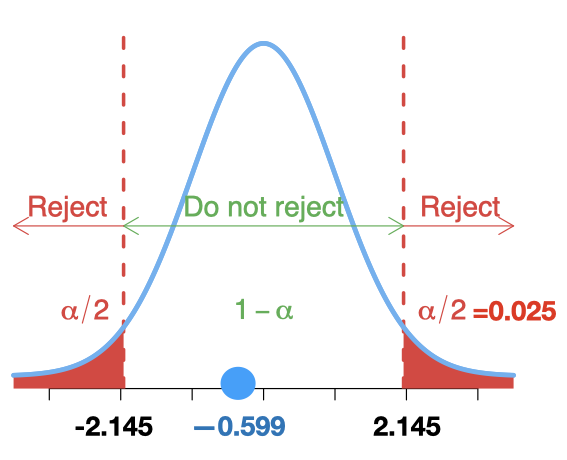
\includegraphics[width=0.9\linewidth,height=0.9\textheight]{hypoex} \end{center}

\textbf{R output:}

%\begin{Shaded}
\begin{Highlighting}[]
\CommentTok{\# Data}
\NormalTok{mlg}\OtherTok{\textless{}{-}}\FunctionTok{c}\NormalTok{(}\FloatTok{27.3}\NormalTok{, }\FloatTok{30.9}\NormalTok{, }\FloatTok{25.9}\NormalTok{, }\FloatTok{31.2}\NormalTok{, }\FloatTok{29.7}\NormalTok{, }
\FloatTok{28.8}\NormalTok{, }\FloatTok{29.4}\NormalTok{, }\FloatTok{28.5}\NormalTok{, }\FloatTok{28.9}\NormalTok{, }\FloatTok{31.6}\NormalTok{,}
\FloatTok{27.8}\NormalTok{, }\FloatTok{27.8}\NormalTok{, }\FloatTok{28.6}\NormalTok{, }\FloatTok{27.3}\NormalTok{, }\FloatTok{27.6}\NormalTok{)}

\CommentTok{\# t{-}test}
\FunctionTok{t.test}\NormalTok{(mlg,}\AttributeTok{alternative =} \StringTok{"two.sided"}\NormalTok{, }\AttributeTok{mu =} \DecValTok{29}\NormalTok{, }\AttributeTok{conf.level =} \FloatTok{0.95}\NormalTok{)}
\end{Highlighting}
%\end{Shaded}

\begin{verbatim}
## 
##  One Sample t-test
## 
## data:  mlg
## t = -0.59878, df = 14, p-value = 0.5589
## alternative hypothesis: true mean is not equal to 29
## 95 percent confidence interval:
##  27.86979 29.63688
## sample estimates:
## mean of x 
##  28.75333
\end{verbatim}

%\begin{Shaded}
\begin{Highlighting}[]
\CommentTok{\# Normality test}
\CommentTok{\# Kolmogorov Smirnov Test}
\FunctionTok{ks.test}\NormalTok{(mlg,}\StringTok{"pnorm"}\NormalTok{, }\AttributeTok{mean=}\FunctionTok{mean}\NormalTok{(mlg), }\AttributeTok{sd=}\FunctionTok{sd}\NormalTok{(mlg))}
\end{Highlighting}
%\end{Shaded}

\begin{verbatim}
## Warning in ks.test(mlg, "pnorm", mean = mean(mlg), sd = sd(mlg)): ties should
## not be present for the Kolmogorov-Smirnov test
\end{verbatim}

\begin{verbatim}
## 
##  One-sample Kolmogorov-Smirnov test
## 
## data:  mlg
## D = 0.13004, p-value = 0.9616
## alternative hypothesis: two-sided
\end{verbatim}

%\begin{Shaded}
\begin{Highlighting}[]
\CommentTok{\# Shapiro{-}Wilk test}
\FunctionTok{shapiro.test}\NormalTok{(mlg) }
\end{Highlighting}
%\end{Shaded}

\begin{verbatim}
## 
##  Shapiro-Wilk normality test
## 
## data:  mlg
## W = 0.95817, p-value = 0.6606
\end{verbatim}

%\begin{Shaded}
\begin{Highlighting}[]
\FunctionTok{par}\NormalTok{(}\AttributeTok{mfrow=}\FunctionTok{c}\NormalTok{(}\DecValTok{1}\NormalTok{,}\DecValTok{2}\NormalTok{))}
\FunctionTok{qqnorm}\NormalTok{(mlg)}
\FunctionTok{qqline}\NormalTok{(mlg, }\AttributeTok{col =} \StringTok{"red"}\NormalTok{)}
\FunctionTok{hist}\NormalTok{(mlg)}
\end{Highlighting}
%\end{Shaded}

\begin{center}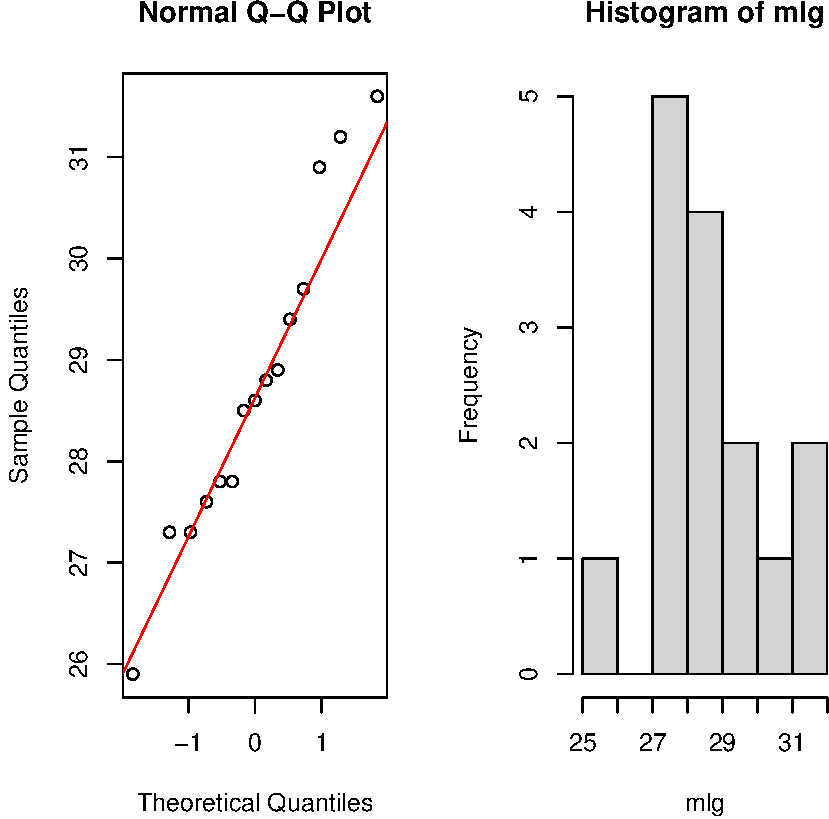
\includegraphics[width=1\linewidth,height=1\textheight]{unnamed-chunk-53-1} \end{center}

\pagebreak

\hypertarget{hypothesis-testing-two-samples}{%
\section{Hypothesis Testing Two
Samples}\label{hypothesis-testing-two-samples}}

\hypertarget{motivation}{%
\subsection{Motivation}\label{motivation}}

We often encounter such statements or claims:

\begin{itemize}
\item
  A newspaper claims that the average starting salary of MBA graduates
  is over \pounds50K. (one sample test)
\item
  A claim about the efficiency of a particular diet program, the average
  weight after the program is less than the average weight before the
  program. (two paired samples test)
\item
  On average female managers earn less than male managers, given that
  they have the same qualifications and skills. (two independent samples
  test)
\end{itemize}

So we have claims about the populations' means (averages) and we would
like to verify or examine these claims.

This is a kind of problem that \textbf{hypothesis testing} is designed
to solve.

\hypertarget{hypothesis-tests-for-two-population-means}{%
\subsection{Hypothesis tests for two population
means}\label{hypothesis-tests-for-two-population-means}}

We have two types of samples here:

\begin{itemize}
\item
  \textbf{Paired samples:} each case must have scores on two variables
  and it is applicable to two types of studies, repeated-measures
  (e.g.~weights before and after a diet plan) and matched-subjects
  designs (e.g.~measurements on twins or child/parent pairs).
\item
  \textbf{Independent samples:} two samples are called independent
  samples if the sample selected from one of the populations has no
  effect on (holds no information about) the sample selected from the
  other population.
\end{itemize}

\(~\)

In order to compare two population means, we are going to test the null
hypothesis \[H_{0} :\mu _{1} =\mu _{2} \]

against one of the following alternatives:

\begin{itemize}
\item
  \(H_1:\mu_1\neq\mu_2\;\) or \(\;\mu_1-\mu_2\neq 0\) (Two-tailed)
\item
  \(H_1:\mu_1<\mu_2\;\) or \(\;\mu_1-\mu_2< 0\) (Left-tailed)
\item
  \(H_1:\mu_1>\mu_2\;\) or \(\;\mu_1-\mu_2> 0\) (Right-tailed)
\end{itemize}

\hypertarget{comparing-two-means-paired-related-samples}{%
\subsection{Comparing two means: Paired (related)
samples}\label{comparing-two-means-paired-related-samples}}

\begin{itemize}
\item
  \textbf{Assumptions:} the paired differences, \(d = x_1- x_2\), are
  normally distributed.
\item
  Test statistics: \textbf{Paired t-test}
  \[t=\frac{\bar{d}}{s_{d} /\sqrt{n} } \] where
  \(\bar{d}=\frac{1}{n}\sum d_{i} \quad and\quad s_d^2 =\frac{1}{n-1}\sum (d{}_{i} -\bar{d})^{2}\)
\item
  \(100(1- \alpha)\%\) confidence intervals for the difference between
  two population means \(\mu_{1} -\mu_{2}\) are
  \[\bar{d}\pm t_{\alpha/2} \;\; s_{d} /\sqrt{n} \] where
  \(t_{\alpha/2}\) is the \(\alpha/2\) critical value from the
  t-distribution with \(df = n-1\)
\end{itemize}

\hypertarget{comparing-two-means-independent-samples}{%
\subsection{Comparing two means: Independent
samples}\label{comparing-two-means-independent-samples}}

In order to test \(H_0:\mu_1=\mu_2\) for two independent samples, we
need to use one of the following test statistics, we should choose the
one that satisfies the assumptions. Let \(\sigma_1\) and \(\sigma_2\) be
the standard deviations of population 1 and population 2, respectively.

\hypertarget{z-test}{%
\subsubsection{z-test}\label{z-test}}

\begin{itemize}
\item
  Assumptions: \(\sigma_1\) and \(\sigma_2\) are known and we have large
  samples (\(n_1\geq30\), \(n_2\geq30\))
\item
  Test statistic: \textbf{z-test}
  \[z=\frac{\bar{x}_{1} -\bar{x}_{2} }{\sqrt{(\sigma_1^2 /n_1 )+(\sigma_2^2 /n_2 )} } \]
\item
  \(100(1- \alpha)\%\) confidence intervals for the difference between
  two population means \(\mu_{1} -\mu_{2}\) are
  \[(\bar{x}_{1} -\bar{x}_{2} )\pm z_{\alpha /2} \; \sqrt{(\sigma_{1}^{2} /n_{1} )+(\sigma_{2}^{2} /n_{2} )} \]
\end{itemize}

where \(z_{\alpha/2}\) is the \(\alpha/2\) critical value from the
standard normal distribution.

\hypertarget{pooled-t-test}{%
\subsubsection{Pooled t-test}\label{pooled-t-test}}

\begin{itemize}
\item
  Assumptions: Normal populations, \(\sigma_1\) and \(\sigma_2\) are
  unknown but equal (\(\sigma_1 = \sigma_2\))
\item
  Test statistic: \textbf{Pooled t-test}
  \[t=\frac{\bar{x}_{1} -\bar{x}_{2} }{s_{p} \; \sqrt{(1/n_{1} )+(1/n_{2} )} } \]
  has a t-distribution with \(df=n_{1} +n_{2} -2\), where
  \(s_{p} =\sqrt{\frac{(n_{1} -1)s_{1}^{2} +(n_{2} -1)s_{2}^{2} }{n_{1} +n_{2} -2} }\).
\item
  \(100(1- \alpha)\%\) confidence intervals for the difference between
  two population means \(\mu_{1} -\mu_{2}\) are
  \[(\bar{x}_{1} -\bar{x}_{2} )\pm t_{\alpha /2} \; s_{p} \sqrt{(1/n_{1} )+(1/n_{2} )} \]
  where \(t_{\alpha/2}\) is the \(\alpha/2\) critical value from the
  t-distribution with \(df=n_{1} +n_{2} -2\).
\end{itemize}

\hypertarget{non-pooled-t-test}{%
\subsubsection{Non-Pooled t-test}\label{non-pooled-t-test}}

\begin{itemize}
\item
  Assumptions: Normal populations, \(\sigma_1\) and \(\sigma_2\) are
  unknown and unequal (\(\sigma_1 \neq \sigma_2\))
\item
  Test statistic: \textbf{Non-Pooled t-test}
  \[t=\frac{\bar{x}_{1} -\bar{x}_{2} }{\sqrt{(s_{1}^{2} /n_{1} )+(s_{2}^{2} /n_{2} )} } \]
  has a t-distribution with
  \(df=\Delta=\frac{[(s_{1}^{2} /n_{1} )+(s_{2}^{2} /n_{2} )]^{2} }{\left[\frac{(s_{1}^{2} /n_{1} )^{2} }{n_{1} -1} +\frac{(s_{2}^{2} /n_{2} )^{2} }{n_{2} -1} \right]}\)
\item
  100(1- \(\alpha\))\% confidence intervals for the difference between
  two population means \(\mu_{1} -\mu_{2}\) are
  \[(\bar{x}_{1} -\bar{x}_{2} )\pm t_{\alpha /2} \; \sqrt{(s_{1}^{2} /n_{1} )+(s_{2}^{2} /n_{2} )} \]
  where \(t_{\alpha/2}\) is the \(\alpha/2\) critical value from the
  t-distribution with \(df =\Delta\).
\end{itemize}

\hypertarget{levenes-test-for-equality-of-variances}{%
\subsubsection{Levene's Test for Equality of
Variances}\label{levenes-test-for-equality-of-variances}}

In order to choose between Pooled t-test and Non-Pooled t-test, we need
to check the assumption that the two populations have equal (but
unknown) variances. That is, test the null hypothesis that
\(H_0:\sigma^2_1=\sigma^2_2\) against the alternative that
\(H_1:\sigma^2_1\neq \sigma^2_2\).

The test statistic of Levene's test follows \(F\) distribution with
\(1\) and \(n_1+n_2-2\) degrees of freedom.

\begin{center}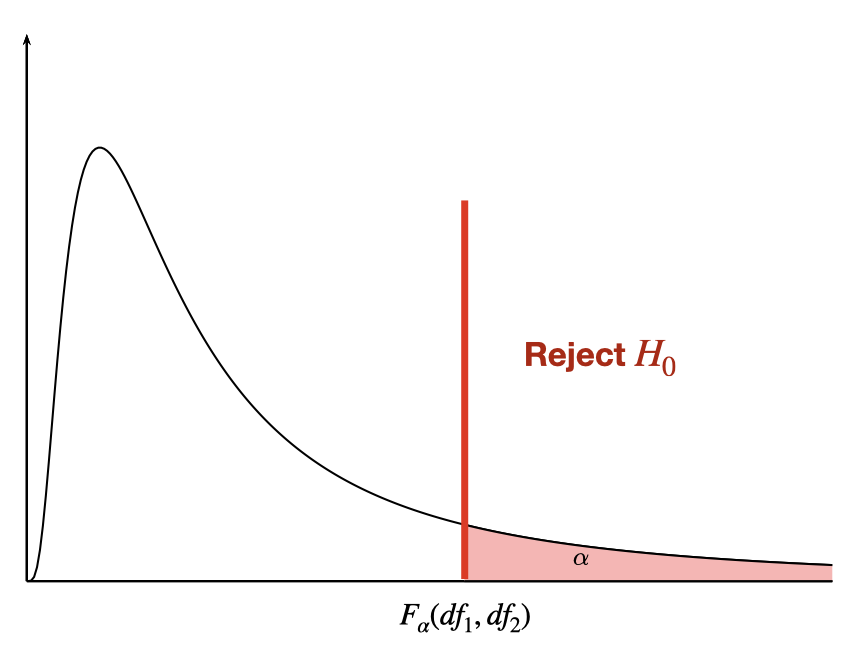
\includegraphics[width=1\linewidth,height=1\textheight]{Ftest} \end{center}

\hypertarget{critical-value-approach-to-hypothesis-testing-1}{%
\subsection{Critical-value approach to hypothesis
testing}\label{critical-value-approach-to-hypothesis-testing-1}}

\begin{enumerate}
\def\labelenumi{\arabic{enumi}.}
\item
  State the null and alternative hypotheses
\item
  Decide on the significance level \(\alpha\)
\item
  Compute the value of the test statistic
\item
  Determine the critical value(s)
\item
  If the value of the test statistic falls in the rejection region,
  reject \(H_0\); otherwise do not reject \(H_0\).
\item
  Interpret the result of the hypothesis test.
\end{enumerate}

We can replace Steps 4 and 5 by using the p-value. A common rule of
thumb is that we reject the null hypothesis if the p-value is less than
or equal to the significance level \(\alpha\).

For \(z\)-test:

\begin{center}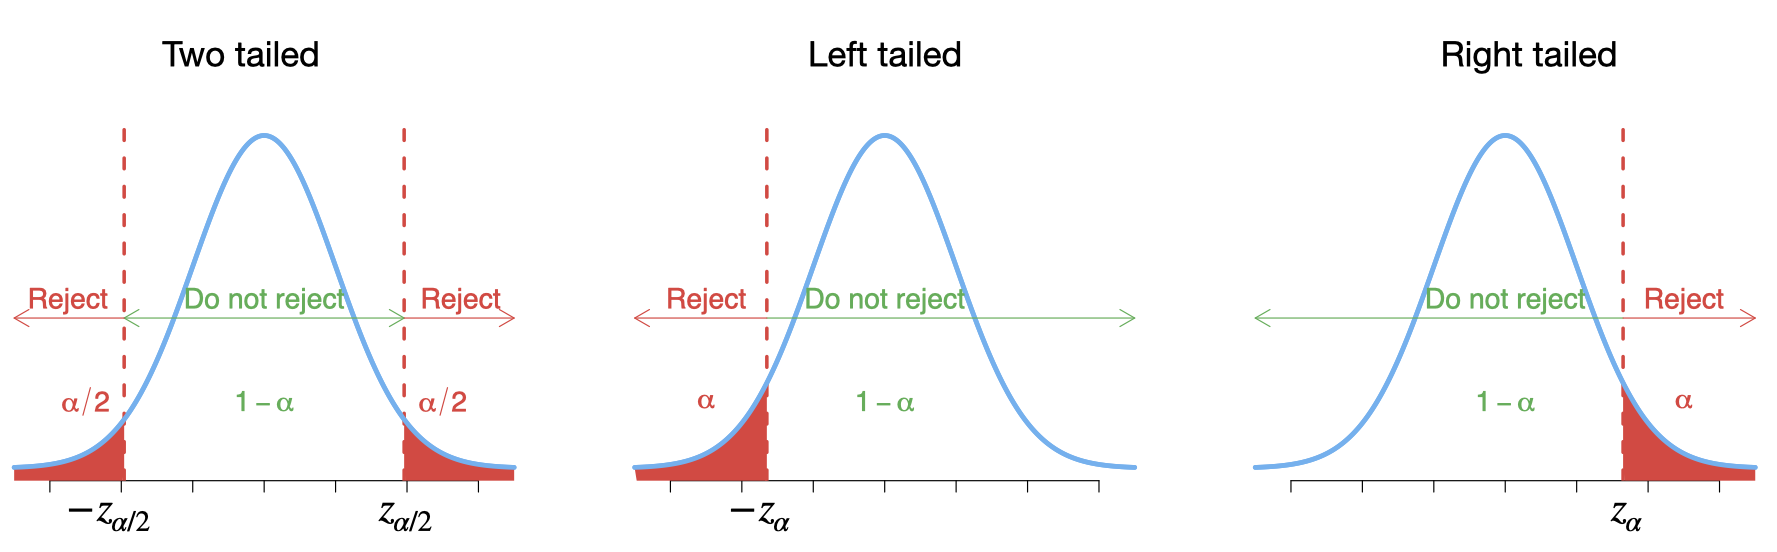
\includegraphics[width=1\linewidth,height=1.3\textheight]{hytestz1} \end{center}

For any specific significance level \(\alpha\), one can obtain these
critical values \(\pm z_{\alpha/2}\) and \(\pm z_{\alpha}\) from the
standard normal distribution table. If the value of the test statistic
falls in the rejection region, reject \(H_0\); otherwise do not reject
\(H_0\).

\begin{longtable}[]{@{}lllll@{}}
\toprule()
\(z_{0.10}\) & \(z_{0.05}\) & \(z_{0.025}\) & \(z_{0.01}\) &
\(z_{0.005}\) \\
\midrule()
\endhead
1.282 & 1.645 & 1.96 & 0 & 2.326 2.576 \\
\bottomrule()
\end{longtable}

For \(t\)-test:

\begin{center}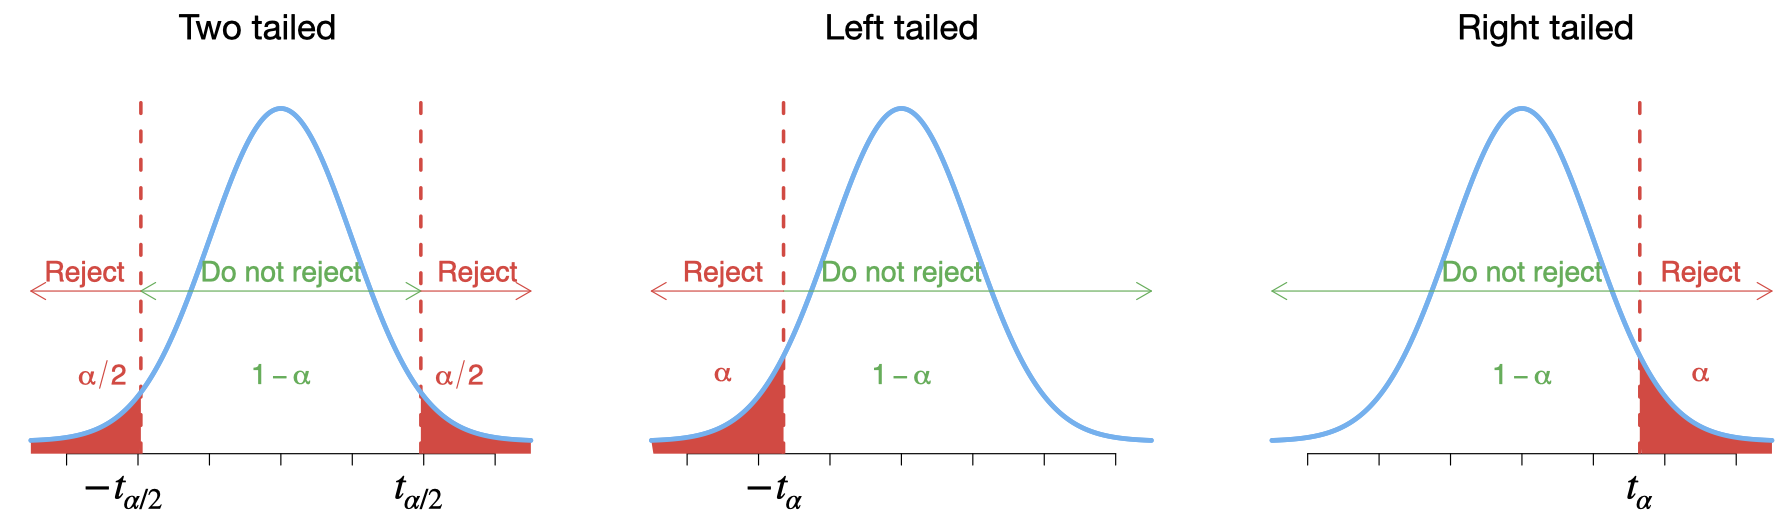
\includegraphics[width=1\linewidth,height=1.3\textheight]{hytestt} \end{center}

For any specific significance level \(\alpha\), one can obtain these
critical values \(\pm t_{\alpha/2}\) and \(\pm t_{\alpha}\) from the T
distribution table. For example, for \(df=9\) and \(\alpha=.05\), the
critical values are \(\pm t_{0.025}=\pm 2.262\) and
\(\pm t_{0.05}=\pm 1.833\).

\hypertarget{example-4}{%
\subsection{Example}\label{example-4}}

In a study of the effect of cigarette smoking on blood clotting, blood
samples were gathered from 11 individuals before and after smoking a
cigarette and the level of platelet aggregation in the blood was
measured. Does smoking affect platelet aggregation?

\begin{longtable}[]{@{}ccc@{}}
\toprule()
before & after & d \\
\midrule()
\endhead
25 & 27 & 2 \\
25 & 29 & 4 \\
27 & 37 & 10 \\
44 & 56 & 12 \\
30 & 46 & 16 \\
67 & 82 & 15 \\
53 & 57 & 4 \\
53 & 80 & 27 \\
52 & 61 & 9 \\
60 & 59 & -1 \\
28 & 43 & 15 \\
\bottomrule()
\end{longtable}

\[\bar{d}=\frac{1}{n}\sum_{i=1}^nd_i=10.27\] \[s_d=7.98\]
\[s_{\bar{d}}=\frac{s_d}{\sqrt{n}}=\frac{7.98}{\sqrt{11}}=2.40\]

At the 90\% level (\(\alpha=0.10\)), the critical value
\(t_{10,0.05}=1.812\), and so a 90\% confidence interval is

\[\bar{d}\pm 1.812\;(s_d/\sqrt{n})=10.27\pm1.812\times 2.40=[5.19,14.63]\]

which clearly excludes 0.

To test the null hypothesis that the means before and after are the
sample: that is \(H_0:\mu_{before}=\mu_{after}\) against
\(H_1:\mu_{before}\neq\mu_{after}\)
\[t=\frac{\bar{d}}{s_d/\sqrt{n}}=\frac{10.27}{2.40}=4.28\] since
\(|t|>1.812\) then we reject \(H_0\).

\begin{center}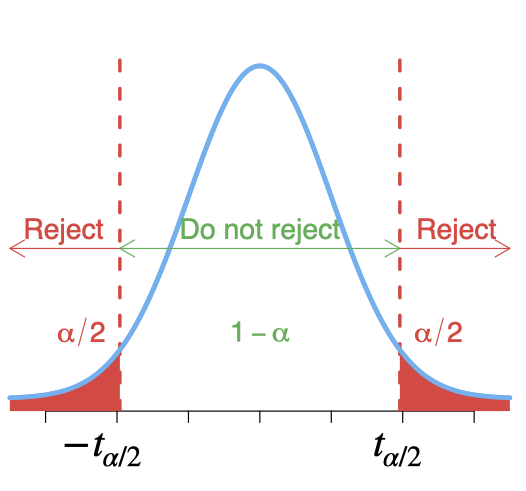
\includegraphics[width=1\linewidth,height=1\textheight]{Ttest2} \end{center}

%\begin{Shaded}
\begin{Highlighting}[]
\NormalTok{before}\OtherTok{\textless{}{-}}\FunctionTok{c}\NormalTok{(}\DecValTok{25}\NormalTok{,}\DecValTok{25}\NormalTok{,}\DecValTok{27}\NormalTok{,}\DecValTok{44}\NormalTok{,}\DecValTok{30}\NormalTok{,}\DecValTok{67}\NormalTok{,}\DecValTok{53}\NormalTok{,}\DecValTok{53}\NormalTok{,}\DecValTok{52}\NormalTok{,}\DecValTok{60}\NormalTok{,}\DecValTok{28}\NormalTok{)}
\NormalTok{after}\OtherTok{\textless{}{-}}\FunctionTok{c}\NormalTok{(}\DecValTok{27}\NormalTok{,}\DecValTok{29}\NormalTok{,}\DecValTok{37}\NormalTok{,}\DecValTok{56}\NormalTok{,}\DecValTok{46}\NormalTok{,}\DecValTok{82}\NormalTok{,}\DecValTok{57}\NormalTok{,}\DecValTok{80}\NormalTok{,}\DecValTok{61}\NormalTok{,}\DecValTok{59}\NormalTok{,}\DecValTok{43}\NormalTok{)}
\NormalTok{d}\OtherTok{\textless{}{-}}\NormalTok{after}\SpecialCharTok{{-}}\NormalTok{before}
\FunctionTok{qt}\NormalTok{(}\FloatTok{0.1}\SpecialCharTok{/}\DecValTok{2}\NormalTok{, }\AttributeTok{df=}\DecValTok{10}\NormalTok{)}
\end{Highlighting}
%\end{Shaded}

\begin{verbatim}
## [1] -1.812461
\end{verbatim}

%\begin{Shaded}
\begin{Highlighting}[]
\FunctionTok{t.test}\NormalTok{(after, before, }\StringTok{"two.sided"}\NormalTok{, }\AttributeTok{paired =} \ConstantTok{TRUE}\NormalTok{,}\AttributeTok{conf.level =} \FloatTok{0.90}\NormalTok{)}
\end{Highlighting}
%\end{Shaded}

\begin{verbatim}
## 
##  Paired t-test
## 
## data:  after and before
## t = 4.2716, df = 10, p-value = 0.001633
## alternative hypothesis: true difference in means is not equal to 0
## 90 percent confidence interval:
##   5.913967 14.631488
## sample estimates:
## mean of the differences 
##                10.27273
\end{verbatim}

%\begin{Shaded}
\begin{Highlighting}[]
\FunctionTok{hist}\NormalTok{(d,}\AttributeTok{main=}\StringTok{""}\NormalTok{,}\AttributeTok{col =} \StringTok{\textquotesingle{}\#61B2F2\textquotesingle{}}\NormalTok{)}
\end{Highlighting}
%\end{Shaded}

\begin{center}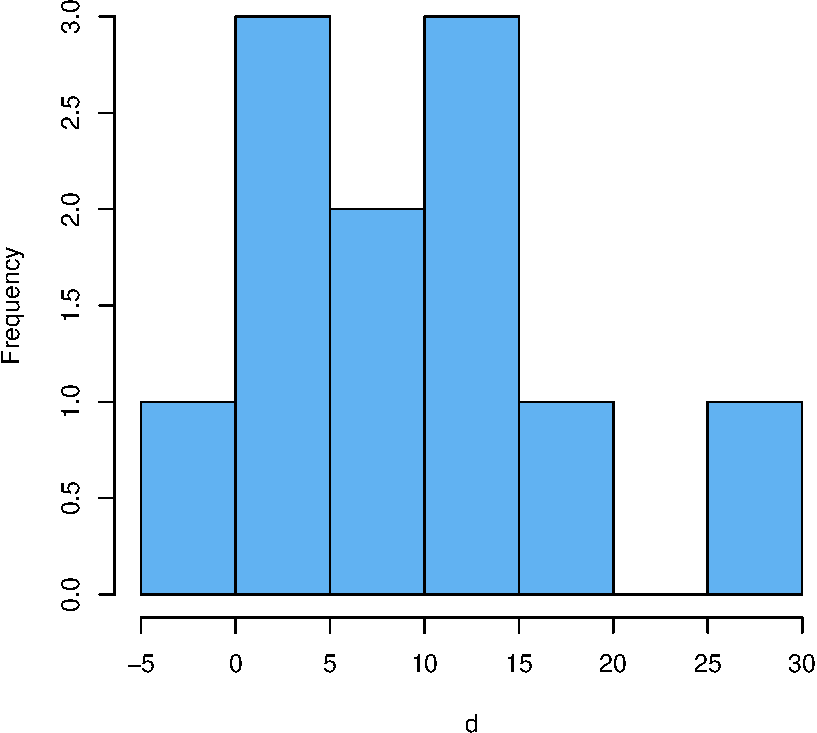
\includegraphics[width=1\linewidth,height=1\textheight]{unnamed-chunk-59-1} \end{center}

%\begin{Shaded}
\begin{Highlighting}[]
\FunctionTok{qqnorm}\NormalTok{(d, }\AttributeTok{pch =} \DecValTok{1}\NormalTok{)}
\FunctionTok{qqline}\NormalTok{(d, }\AttributeTok{col =} \StringTok{"steelblue"}\NormalTok{, }\AttributeTok{lwd =} \DecValTok{2}\NormalTok{)}
\end{Highlighting}
%\end{Shaded}

\begin{center}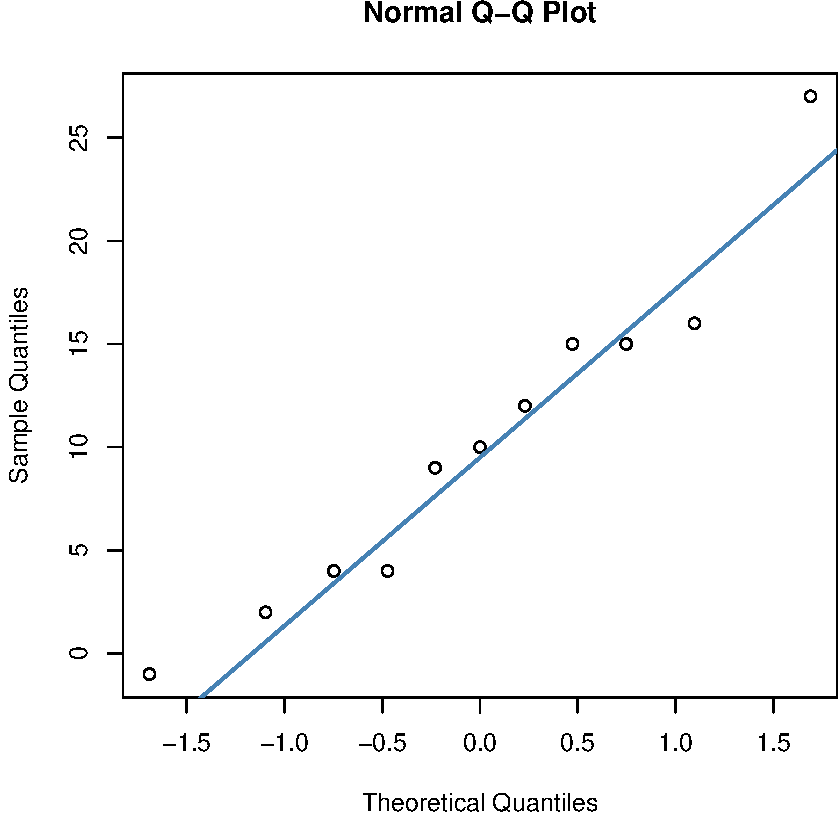
\includegraphics[width=1\linewidth,height=1\textheight]{unnamed-chunk-59-2} \end{center}

\pagebreak

\hypertarget{nonparametric-tests}{%
\section{Nonparametric Tests}\label{nonparametric-tests}}

\hypertarget{wilcoxon-signed-rank-test-paired-samples}{%
\subsection{Wilcoxon signed-rank test (Paired
samples)}\label{wilcoxon-signed-rank-test-paired-samples}}

If the population of all paired differences \(d\) is symmetric but not
necessarily normal, then we should use a nonparametric test called
\textbf{Wilcoxon signed-rank test} in order to compare the two
populations, i.e.~to test \(H_0\): no group difference.

To calculate the Wilcoxon signed-rank test statistic:

\begin{itemize}
\item
  Calculate all paired differences.
\item
  Rank the absolute differences, that is ignoring the sign, after
  excluding the zeros.
\item
  Sum the ranks of the positive and negative differences.
\item
  The Wilcoxon signed-rank test \(V\) is the minimum of these two sums.
  That is \[V=\min(V^+,V^-)\] where \(V^+\) is the sum of the ranks of
  the absolute differences for all pairs with positive difference, and
  \(V^-\) is the equivalent for negative differences.
\item
  We can then compare \(V\) to the critical value, \(T\) , for a given
  significance level, \(\alpha\) , and number of non-zero differences,
  \(n\), from the statistical table.
\item
  We reject \(H_0\) at level \(\alpha\) if \(V<T\).
\end{itemize}

Under \(H_0\) and assuming no ties, \(V\) has the following properties:

\begin{itemize}
\item
  \(E[V] = \mu_{V} = \frac{1}{4}n(n+1)\).
\item
  \(Var[V] = \sigma^2_{V} = \frac{1}{24} n(n+1)(2n+1)\).
\item
  The distribution of \(V\) is symmetric about \(\mu_{V}\).
\item
  For large \(n\), \(V \sim N(\mu_{V}, \sigma^2_{V})\).
\end{itemize}

So the standardize version of this test statistic is
\[Z=\frac{V-\frac{n(n+1)}{4}}{\sqrt{\frac{n(n+1)(2n+1)}{24}}}\]

\hypertarget{example-5}{%
\subsection{Example}\label{example-5}}

Consider a sample of five students' grades in Finance and Accounting. We
are interested in testing whether the students' grades in finance is
lower than the students' grades in accounting, so we have a left-tailed
test. Use \(\alpha=10\%\).

\begin{longtable}[]{@{}cccc@{}}
\toprule()
\(x_1\) & \(x_2\) & \(x_1-x_2\) & rank of \(|x_1-x_2|\) \\
\midrule()
\endhead
73 & 88 & -15 & 3 \\
51 & 60 & -9 & 2 \\
85 & 65 & 20 & 4 \\
65 & 66 & -1 & 1 \\
70 & 70 & 0 & - \\
\bottomrule()
\end{longtable}

The Wilcoxon signed-rank test has value \(V=\min(6,4)=4\).

We compare this value to the critical value \(T=1\) obtained using R,
\texttt{qsignrank(0.1,4)}, or we can use the p-value as below (using R).

%\begin{Shaded}
\begin{Highlighting}[]
\NormalTok{x1}\OtherTok{\textless{}{-}}\FunctionTok{c}\NormalTok{(}\DecValTok{73}\NormalTok{,}\DecValTok{51}\NormalTok{,}\DecValTok{85}\NormalTok{,}\DecValTok{65}\NormalTok{,}\DecValTok{70}\NormalTok{)}
\NormalTok{x2}\OtherTok{\textless{}{-}}\FunctionTok{c}\NormalTok{(}\DecValTok{88}\NormalTok{,}\DecValTok{60}\NormalTok{,}\DecValTok{65}\NormalTok{,}\DecValTok{66}\NormalTok{,}\DecValTok{70}\NormalTok{)  }
\FunctionTok{wilcox.test}\NormalTok{(x1,x2,}\AttributeTok{paired=}\ConstantTok{TRUE}\NormalTok{, }\AttributeTok{alternative =} \StringTok{"less"}\NormalTok{) }
\end{Highlighting}
%\end{Shaded}

\begin{verbatim}
## Warning in wilcox.test.default(x1, x2, paired = TRUE, alternative = "less"):
## cannot compute exact p-value with zeroes
\end{verbatim}

\begin{verbatim}
## 
##  Wilcoxon signed rank test with continuity correction
## 
## data:  x1 and x2
## V = 4, p-value = 0.4276
## alternative hypothesis: true location shift is less than 0
\end{verbatim}

\(~\)\\
As the \(p\)-value is large we do not reject \(H_0\).

\(~\)

\hypertarget{wilcoxon-rank-sum-test-independent-samples}{%
\subsection{Wilcoxon rank-sum test (Independent
samples)}\label{wilcoxon-rank-sum-test-independent-samples}}

If the two (independent) samples are not normally distributed then we
should use a nonparametric test called the \textbf{Wilcoxon rank-sum
test} or alternatively the \textbf{Mann-Whitney U test}.

To calculate the Wilcoxon rank-sum test:

\begin{itemize}
\item
  First combine the two samples into one sample.
\item
  Rank the combined sample.
\item
  Calculate the sum of ranks corresponding to the first sample (we can
  also choose the second sample).
\item
  Wilcoxon rank-sum test is the sum of ranks of the first sample.
\end{itemize}

\(~\)

Let the ranks of the first sample in the combined sample be
\(r_1,\ldots,r_n\) which are all integers from the set
\(\{1,\ldots,N\}\), where \(N=n+m\).

The Wilcoxon rank-sum test statistic is then \[W = \sum_{i=1}^{n} r_i\]

The Mann-Whitney U test statistic is \[W -\frac{n(n+1)}{2}\]

where \(n\) is the number of observations from the first sample, and
\(m\) is the number of observations from the second sample.

When the samples are both large, the distribution of the Wilcoxon
rank-sum statistic is approximately Normal. For large \(n\) and \(m\),
under the null hypothesis of no group differences we have:
\[E[W]=\mu_W=\frac{1}{2} n(n+m+1)\]
\[Var[W]=\sigma^2_W=\frac{1}{12} nm(n+m+1)\]
\[ W\sim N(\mu_W,\sigma^2_W )\] So for large samples, we can use these
values to standardise \(W\) and use standard Normal tables to construct
confidence intervals and test hypotheses.

\hypertarget{example-6}{%
\subsection{Example}\label{example-6}}

Suppose we have two groups of salaries, in thousand of pounds, of women
and men. Test the claim that, on average, women earn less salary than
men, so again we have a left-sided test. Use \(\alpha=5\%\)

\begin{longtable}[]{@{}cc@{}}
\toprule()
Women & Men \\
\midrule()
\endhead
16 & 18 \\
30 & 45 \\
25 & 36 \\
65 & 28 \\
70 & 40 \\
\bottomrule()
\end{longtable}

\begin{itemize}
\item
  First we rank the combined sample.

  \begin{longtable}[]{@{}cc@{}}
  \toprule()
  Combined sample & Rank \\
  \midrule()
  \endhead
  16 & 1 \\
  18 & 2 \\
  25 & 3 \\
  28 & 4 \\
  30 & 5 \\
  36 & 6 \\
  40 & 7 \\
  45 & 8 \\
  \bottomrule()
  \end{longtable}
\item
  We will consider women salaries, and the sum of ranks related to the
  women's group is \(1+3+5=9\).
\item
  For \(n=3\), \(m=5\) and \(\alpha=0.05\), we can obtain the critical
  values from the table, so we have \(T_L=8\) (as we have a left-sided
  test)
\item
  Since \(W=9 \nless T_L=8\), so we do not reject \(H_0\).
\item
  Notice, the value given by \emph{R} is the Mann-Whitney U test, which
  is given by

  Mann-Whitney U test= 9 \(- \frac{3(3+1)}{2}=9-6=3\).
\end{itemize}

\(~\)\\
Or we can use R as follows:

%\begin{Shaded}
\begin{Highlighting}[]
\NormalTok{w}\OtherTok{\textless{}{-}}\FunctionTok{c}\NormalTok{(}\DecValTok{16}\NormalTok{,}\DecValTok{30}\NormalTok{,}\DecValTok{25}\NormalTok{)}
\NormalTok{m}\OtherTok{\textless{}{-}}\FunctionTok{c}\NormalTok{(}\DecValTok{18}\NormalTok{,}\DecValTok{45}\NormalTok{,}\DecValTok{36}\NormalTok{,}\DecValTok{28}\NormalTok{)  }
\FunctionTok{wilcox.test}\NormalTok{(w,m, }\AttributeTok{alternative =} \StringTok{"less"}\NormalTok{) }
\end{Highlighting}
%\end{Shaded}

\begin{verbatim}
## 
##  Wilcoxon rank sum exact test
## 
## data:  w and m
## W = 3, p-value = 0.2
## alternative hypothesis: true location shift is less than 0
\end{verbatim}

\(~\)

Again the p-value is large so we do not reject \(H_0\).

\end{document}
